%% Definir tipo de documento
\documentclass[12pt]{report}
%% tamaño de hoja
\usepackage[letterpaper, margin = 1in]{geometry}
%\usepackage[utf8]{inputenc}
\usepackage[spanish]{babel}
%% Añadir varias imagenes en una sola
\usepackage{graphicx}
\usepackage{epsfig}
\usepackage{caption}
\usepackage{subcaption}
\usepackage{float}
%% Poder citar en APA
\usepackage{natbib}
\bibliographystyle{apalikees}
%% Hipervinculos para las citas y secciones
\usepackage{hyperref}
\hypersetup{
    colorlinks=true,
    linkcolor=black,
    citecolor=black,
    urlcolor=black
}
%% Sub ecuaciones
\usepackage{amsmath}
%% Importar codigo Python
\usepackage{listings}
%% Para la creación de Tablas
\usepackage[normalem]{ulem}
\useunder{\uline}{\ul}{}
\usepackage{longtable}
\usepackage{lipsum}
\captionsetup[table]{name=Tabla}
\usepackage{xcolor,colortbl}
\usepackage{enumitem}
\usepackage{multicol,multirow}
%% Caracteres chinos
\usepackage[UTF8]{ctex}
%% Citas directas
\usepackage{csquotes}
%% Hoja Horizontal
\usepackage{lscape}
%% Evitar los saltos o gaps en las listas
\newcommand\nosep{\vspace{-1ex}\setlength\itemsep{-0.75ex}}
%% Pefileria
\usepackage{marvosym}
\usepackage{amssymb}

%% Documento
\begin{document}
    %%%%%   Hoja de Titulo    %%%%%
    \newcommand{\TitleProject}{\uppercase{Diseño de una maquina herramienta de 3-ejes con tecnología CNC para operaciones de maquinado}}

\newcommand{\AuthorProject}{Carlos Andres Cárdenas Perez\\
        Elías Jose Muñoz Montenegro\\
        Jairo Luis Saenz Benavides\\
        William Sánchez Rosales}
%%%%%   Primera Hoja    %%%%%
\thispagestyle{empty}
\begin{figure}
    \centering
    \includegraphics[scale=0.4]{Cap0_Titulo/EscudoUN.pdf}
\end{figure}

\begin{center}
    \rule{\linewidth}{0.5pt}
        \LARGE{ \textbf{ \TitleProject } }
    \rule{\linewidth}{2pt}
\end{center}
\vspace{2cm}
\begin{center}
    \large
    \textbf{Autores:} \\
        \AuthorProject
\end{center}
\vfill
\begin{center}
    Universidad del Norte\\
    Departamento de Ingeniería Mecánica\\
    Puerto Colombia, Colombia\\
    2019
\end{center}

%%%%%   Hoja en blanco    %%%%%
\newpage
\thispagestyle{empty}
~
\newpage

%%%%%   Segunda Hoja    %%%%%
\thispagestyle{empty}
\begin{center}
        \Large{ \textbf{ \uppercase{\TitleProject} } }
\end{center}
\vspace{2cm}
\begin{center}
    \large 
    \textbf{Autores:} \\
        \textbf{\AuthorProject}
\end{center}
\vspace{2cm}
\begin{center}
    Trabajo de grado presentado como requisito parcial para optar al título de:\\
    \textbf{Ingeniero Mecánico} \\
    \vspace{2cm}
    Tutor: \\
    Ing. Heriberto Enrique Maury Ramirez, PhD\\
    \vspace{2cm}
    Grupo de Investigación:\\
    Laboratorio de Diseño y mecánica de máquinas\\
    \vfill
    Universidad del Norte\\
    División de Ingenierías\\
    Departamento de Ingeniería Mecánica\\
    Puerto Colombia, Colombia\\
    2019
\end{center}
    \newpage
    
    %%%%%   Contenido    %%%%%
    \renewcommand{\contentsname}{Contenido}
    \tableofcontents
    \newpage
    
    %%%%%   Lista de Tablas    %%%%%
    \renewcommand{\listtablename}{Lista de Tablas}
    \addcontentsline{toc}{chapter}{\numberline{}Lista de Tablas}
    \listoftables
    \newpage
    
    %%%%%   Lista de Figuras    %%%%%
    \renewcommand{\listfigurename}{Lista de Figuras}
    \addcontentsline{toc}{chapter}{\numberline{}Lista de Figuras}
    \listoffigures
    \newpage
    \newpage
    %%%%%   Resumen Ejecutivo    %%%%%
    \addcontentsline{toc}{chapter}{\numberline{}Resumen Ejecutivo}
    \chapter*{Resumen Ejecutivo}
En barraquilla, el sector metal-mecánico encargado de operaciones de mecanizado como el fresado y torneado con máquinas CNC es limitado, lo que se traduce en un pobre desarrollo en la industria metal-mecánica. El manejo limitado de la maquinaria CNC para mecanizado se debe al elevado costo de los equipos que se requieren para el mecanizado de piezas con geometría compleja y altas tolerancias de fabricación. En el departamento del atlántico según \cite{lora2012determinantes} tiene un 4\% de participación en la industria metal-mecánica. Viendo el porcentaje de la industria en el atlántica se observa una oportunidad de negocio, donde se plantea la idea de diseñar una maquina CNC para fresado de tres ejes con la cual se trabajarían aluminios y aceros dúctiles con un bajos costo de inversión y con una disminución en consumo de energía durante la operación. Con este fin los estudiantes de pregrado de la universidad del norte se han propuesto a diseñar una maquina herramienta de tres ejes para mecanizado.

El presente trabajo cubre un marco teórico donde se describen los procesos de mecanizado, las fases de diseño conceptual, diseño básico y diseño de detalle de una maquina herramienta CNC para fresado, enfocado principalmente al direccionamiento de los componentes de la arquitectura del mecanismo que siguen las trayectorias de la operación, siguiendo la metodología \cite{dieter2012engineering}. El proyecto comenzó con el planteamiento del problema, una revisión del estado del arte, de la técnica y una revisión de patentes; donde se encontraron opciones de arquitecturas y puntos donde se puede mejorar algo ya existente, la definición de requerimientos y especificaciones utilizando el método de despliegue de la función de la calidad (QFD). Posteriormente se realizó una descomposición funcional donde se identificaron las funciones de primer, segundo y tercer nivel, teniendo así tres alternativas de la solución teniendo en cuentas diferentes concetos de la solución para cada función. Las tres alternativas generadas se evaluaron con el método AHP. Por último, se realizó el diseño básico y detallado de la alternativa seleccionada.

Como resultado del proyecto realizado se determinó el uso como mecanismo de actuación una arquitectura de robot paralelo RRPRR basado en \cite{petko2005mechatronic} con la cual se busca una disminución de los costos de consumo energético, una precisión competitiva y un costo de adquisición menor en comparación maquinas CNC con similar espacio de trabajo que se encuentran en el mercado actual. Además, se lograron tener dimensiones optimas del mecanismo con el uso de algoritmos genéticos.

    
    %%%%%   Capitulo 1 : Formulacion del Proyecto    %%%%%
    \chapter{Formulación del Proyecto}
%%%%%   Resumen    %%%%%
\section{Resumen Ejecutivo}
    
\newpage

%%%%%   Planteamiento del Problema    %%%%%
\section{Planteamiento del Problema}

    En el sector de la industria metal-mecánica en Barranquilla, el costo de la maquinaria para el mecanizado es una de las principales problemáticas para el desarrollo industrial,  debido a que estos requieren costosos equipos de altos niveles desempeño y operabilidad, para satisfacer las geometrias complejas de las piezas a manufacturar.
    
   
    %Una de las principales problemáticas que se presentan en la industria metal-mecánica en Barranquilla, es el costo de la maquinaria que se requiere para fabricar piezas a través del proceso de mecanizado, lo que conlleva a la dificultad de manufacturar piezas con geometría compleja y especifica.   
    
    En Colombia, de acuerdo con \cite{lora2012determinantes} en el 2009 existieron 9,135 establecientes dedicado a la industria, Donde el 17\% (1,618) corresponde al sector metal mecánico. De estos 1,618 establecimientos de metalmecánica según \cite{lora2012determinantes} 1,521 pertenecen a las Pymes (Pequeñas y medianas empresas). Estas se distribuyen con 51\% en Bogotá y Cundinamarca, Antioquia con 18\%, valle del cauca 14\%, Atlántico con un 4\% y el 13\% se distribuye en los demás departamentos. En el país, la producción de piezas metalmecánicas se lleva a cabo a través de procesos de fabricación tradicionales, tales como la fundición, extrusión, laminados, rolado, entre otros; los cuales son limitados con respecto a la complejidad de las piezas a fabricar y/o con el acabado deseado en algunos casos. Las piezas de geometría compleja en la industria barranquillera, generalmente son fabricadas a través de fundición, la cual, en una producción en masa es una opción acertada, ya que según \cite{groover2007fundamentals} algunos procesos por fundición son capaces de producir pieza de forma neta, como la fundición en molde permanente, donde las tolerancias y acabados superficiales no requieren procesos posteriores para llevar la pieza a fin, pero cuando se requiere una pieza específica estos procesos se vuelven ineficientes, dado que los costos de dicho proceso son altos. Sin embargo, de acuerdo con \cite{groover2007fundamentals} hay otros procesos de fundición que son más económicos, como la fundición con molde desechable que sirven para dar una forma inicial a la pieza para un proceso posterior, para obtener las tolerancias y acabados requeridos, como el mecanizado.
    
    Por lo que el mecanizado, como un proceso intermedio-final, permite obtener piezas con geometrías complejas con excelentes acabados superficiales. Pese a esto, es un bajo número de empresas o lugares que cuentan con este tipo de proceso, debido a los considerables costos iniciales y operativos de una máquina herramienta automatizada. A causa de esto, una relevante cantidad de empresas implementan el mecanizado manual; el cual otorga piezas de baja calidad (comparada con las producidas con las CNC), aumenta el tiempo de manufactura, incrementa los costos de mano de obra, demanda personal calificado y no permite un alto nivel de competitividad en el mercado internacional.
    
    Esta problemática afecta directamente a las Pymes, ya que estas no cuentan con los suficientes recursos para adquirir herramientas automatizadas de mecanizado como un centro de mecanizado de 5 ejes que según lo consultado en \citep{Alibaba2019} tiene un precio de 10000 a 20000 dólares.  Entre las consecuencias que esta problemática conlleva, encontramos el lento crecimiento de las Pymes, debido a que estas deben recurrir a fabricantes o proveedores externos ya industrializados al momento de necesitar piezas específicas, elevando así los costos en general y reduciendo las ganancias y creando así cierta dependencia. Por otra parte, podemos encontrar la baja competitividad que tiene el mercado nacional con respecto a el mercado global, debido a la dificultad de crear piezas de alta calidad que cumplan con los estándares internacional.
    
    El objetivo de este proyecto es proponer una máquina herramienta de bajo costo para la funcion de fresado empleando tecnología de robots y de control automatizado; que permitan impulsar el sector metalmecánico del país como de la ciudad, al fortalecer las capacidades de manufacturación de la PyME. Todo esto con el fin de tecnificar e innovar los procesos en estas empresas que conlleven a su crecimiento económico, además de desarrollar sus capacidades de innovación. De todo lo anterior, se plantea la pregunta de investigación: ¿Es posible desarrollar una máquina herramienta economica que permita impulsar las PyME de la industria metalmecánica barranquillera?
 \newpage
 
%%%%%   Justificacion del Proyecto    %%%%%
\section{Justificacion del Proyecto}
    En la actualidad, Colombia posee una industria manufacturera muy diversificada, la cual presenta negocios en sectores como el alimenticio, caucho – plástico, químico, metalmecánico, entre otros; además de lograr producir alrededor de 74.500.000 millones de pesos \citep{DANE2015}, de los cuales el 73\% es producido en las principales ciudades del país, Bogotá, Medellín, Cali y Barranquilla. En el caso del departamento del Atlántico, el 65\% de las empresas manufactureras entran en la categoría de PyME, generando 55\% del valor de producción local. De igual manera, el departamento es capaz de generar exportaciones con valores de US\$1.400 millones, solo en el año 2015, en donde 91\% de estas son producidas por el sector manufacturera, siendo estos repartidos entre el sector químico, con un 41\%, otras industrias, con 21\%, bienes metalmecánicos, 11.6\% \citep{lechuga2018analisis}.
    
    Pese a la importante participación del Atlántico en el sector manufacturera, este solo es capaz de generar el 7.2\% del total nacional; esto debido a que el 65\% de sus empresas son PyME, según lo mostrado por \cite{camargo2017capacidad}, todavía les falta reforzar retos de la gestión y operación, que les otorgue más capacidades dinámicas de innovación y adaptabilidad a los entornos dinámicos. Así mismo, el interés por mejorar las capacidades de innovación de las pequeñas y medianas empresas (PyME) es debida a que estas son pieza fundamental para el desarrollo económico del país, y al incrementar su nivel de competitividad y productividad les permitirá afrontar de manera eficaz los desafíos del mercado internacional mediante el desarrollo de nuevos productos y/o servicios.
    
    Debido a todo lo anterior, el presente proyecto nace como una respuesta a esta problemática, en donde se propone el desarrollo de tecnología CNC para las pequeñas y medianas empresas enfocadas del sector metalmecánico en el departamento; que les permita desarrollar nuevos productos a bajo costo, sin importar el nivel de complejidad de la geometría de las piezas, conservando la calidad de exportación. Obteniendo la región un desarrollo económico, tanto en su sector manufacturero como en los demás sectores que se beneficien de este. 
    
    Por lo tanto, el proyecto plantea el diseño de una máquina herramienta de 3-ejes que permita la fabricación de piezas de alta complejidad geométrica al ser controladas por medio de un computador y de un mecanismo que le otorgue menores requerimientos energéticos, además poseer elementos más ligeros y así reducir tanto los costos iniciales como operativos.
    
%%%%%   Marco Conceptual    %%%%%
\newpage
\section{Marco Conceptual}
\subsection{Proceso de Mecanizado}
Los procesos de maquinado convencional hacen parte de la rama más importante de la familia de procesos de remoción de materia donde también hacen parte los procesos abrasivos, donde de forma mecánica se remueve materia mediante la acción de partículas duras y los procesos no tradicionales, que utilizan otras formas de energía aparte de la herramienta de corte aguda o de partículas abrasivas \citep{groover2007fundamentals}.

El maquinado es un proceso de manufactura donde se remueve un exceso de materia de una pieza de trabajo con el uso de una herramienta de corte, con el fin que el material remanente sea la forma deseada de la pieza. La acción predomínate en este proceso es la formación de viruta mediante la deformación cortante del material. Lo materiales donde es mas frecuentes la implementación de este tipo de procesos son lo metales.La figura \ref{ilustraciondelprocesodemecanizado} se ilustra como es el proceso \citep{groover2007fundamentals}.

\begin{figure}[hbt]
    \centering
    \includegraphics[width = 0.8\textwidth]{Cap1_FormulaciondelProyecto/Figuras/ilustraciondelprocesodemecanizado.PNG}
    \caption{Sección transversal de proceso de maquinado.}
    \citep{groover2007fundamentals}
    \label{ilustraciondelprocesodemecanizado}
\end{figure}


El mecanizada a lo largo de la historia ha sido de los procesos de manufactura el más importante, ya que con el desarrollo de varias de las operaciones de maquinado se puede describir en gran parte la revolución industrial y el crecimiento de las economías basadas en la manufactura. Las siguientes razones exponen la importancia de las operaciones de maquinado desde el punto de vista comercial y tecnológico  \citep{groover2007fundamentals}.\\
\begin{itemize}
\item \textbf{Amplia gama de materiales de trabajo:} El maquinado se puede aplicar a una gran variedad de materiales. Casi todos los metales solidos pueden aplicar a procesos de maquinado, al igual que los compuestos plásticos. Por otro lado, se presentan dificultades al tratar maquinar cerámica por su dureza y fragilidad; no obstante, se puede cortar por medio de maquinado abrasivo\citep{groover2007fundamentals}.

\item\textbf{Variedad de formas y característica geométricas:} El maquina puede ser usado para formar cualquier geometría regular, como superficies planas, agüeros redondos y cilindros. Cuando se introducen variaciones en las trayectorias y forma de las herramientas, se pueden crear formas irregulares, como cuerdas de tornillos y ranuras T.  al implementar en secuencia operaciones de maquinado, se puede producir forma de complejidad y variedad ilimitada\citep{groover2007fundamentals}.

\item\textbf{Precisión dimensional:} El mecanizado puede producir piezas de trabajo con tolerancias muy estrechas de menos de $\pm 0.025$ mm($\pm 0.001$ in). Es más preciso que otros procesos\citep{groover2007fundamentals}.%%te estoy viendo %% EM: hehehehe
\item\textbf{Acabados superficiales de calidad:} Los acabados superficiales con los cuales se puede llegar con el maquinado son mejores que 0.4 micras (16 $\mu$in) \citep{groover2007fundamentals}.
\end{itemize}

Por otra parte, en los procesos de remoción de material existe ciertas desventajas:
\begin{itemize}
    \item \textbf{Desperdicio de material:} El proceso de maquinado es inherentemente un desprecio de materia. En general la viruta generada es la operación es el desprecio. Aunque, por lo general, la viruta generada puede ser reciclada\citep{groover2007fundamentals}.
    \item \textbf{Consumo de tiempo:} El maquinado por lo general toma más tiempo en la formación la pieza que los procesos alternos de formado como el fundido o forjado\citep{groover2007fundamentals}.
\end{itemize}

\section*{Tipos de operaciones de maquinado }

\subsection*{Torneado}

Es la operación de mecanizado se lleva acabo mediante movimientos básicos: el movimiento de corte de material, que es rotativo sobre la pieza, y el movimiento de avance es perpendicular al eje de la rotación y es realizado por la herramienta de corte \citep{Fenoll2009}.\\

\begin{figure}[ht]
    \centering
    \includegraphics[width = 0.8\textwidth]{Cap1_FormulaciondelProyecto/torneado.PNG}
    \caption{Operación de torneado.}
    \citep{groover2007fundamentals}
    %\label{ilustraciondelprocesodemecanizado}
\end{figure}
\subsubsection*{Parámetros de corte del torneado.}

La velocidad de rotación que usa en el torneado esta relacionada con la velocidad de corte requerida en la superficie cilíndrica de la pieza de trabajo por la siguiente ecuación: 

\begin{equation}
    N=\frac{v}{\pi D_{0}}
\end{equation}
Donde $N$: es la velocidad de rotación que dada en, $Rev./min$; $v$:es la velocidad de corte dada en ,$m/min (ft/min)$; y $D_{0}$ : Es el diámetro original de la pieza y está dado en $m(ft)$.

Cuando en la operación de torneado se quiere reducir el diámetro de trabajo $D_{0}$ al diámetro final $D_{f}$ , el cambio de estos destremina la profundidad de corte $d$: 
\begin{equation}
    D_{f}=D_{0}-2d
\end{equation}
El avance en el torneado por lo general se expresa en $mm/rev (in/rev )$. El avance se puede convertir en velocidad de avance lineal en $mm/min$ mediante la fórmula:
\begin{equation}
    f_{r}=Nf
\end{equation}
 donde $f_{r}$: es velocidad de avance y esta dada en $mm/min (in/min)$; y $f$: es avance y esta en $mm/rev (in/rev).$
 
 El tiempo que toma la operación de torneado de una extremo a otro  a una pieza esta dada por:
 
 \begin{equation}
     T_{m}=\frac{L}{f_{r}}
 \end{equation}
 
 donde $T_{m}$ es el tiempo de maquinado en $min$; y L es la longitud de la pieza cilíndrica en $mm (in)$.
Un cálculo más directo del tiempo de maquinado lo proporciona la ecuación siguiente:
 
 \begin{equation}
     T_{m}=\frac{\pi D_{0} L}{f v}
 \end{equation}
La velocidad volumetrica de Remoción de un materia en $mm^{3}/min(in^{3}/min)$ y se puede determinar más convencionalmente con la siguiente ecuación:
\begin{equation}
    R_{MR}=vfd
\end{equation}

\subsubsection*{Trabajos más usuales realizados en un torno}
El torno normalmente es usado en trabajos de cilindrado, el torneado cónico, el refrentado, el roscado, el taladrado y el maleteado \citep{Fenoll2009}.\\
\begin{itemize}
    \item\textbf{ Cilindrado:} Esta operación permite dar forma uniforme a los diámetros de la pieza cilíndrica mediante desplazamientos de la herramienta de corte paralelamente al eje de giro y el corte perpendicular a este. Con el cilindrado se puede reducir diámetros exteriores y aumentar los diámetros interiores \citep{Fenoll2009} (Figura:\ref{fig:Cilintrado}).
    \item\textbf{Torneado cónico:} Esta operación trabaja con un desplazamiento de la cuchilla no paralela al eje de giro dando piezas con formas cónicas \citep{Fenoll2009}(Figura:\ref{fig:torneadoconico}).
    \item\textbf{Refrentado:} Mediante esta operación se logran planos que son perpendiculares al eje de giro \citep{Fenoll2009}(Figura:\ref{fig:Refretado}).
    \item\textbf{Roscado:} Con el torno se pueden lograr mecanizar rosca, tanto para superficies internas como externas y logra una correcta unión de elementos \citep{Fenoll2009}(Figura:\ref{fig:Roscado}).
    \item\textbf{Taladrado:} Esta operación puede lograrse en el torno con lo broca en el cabezal móvil, y solo se puede hacer en el centro de la pieza \citep{Fenoll2009}(Figura:\ref{fig:Taladrado}).
    \item\textbf{Moleteado:} En este proceso, para dar a la pieza la forma deseada, en lugar de utilizar cuchillas se usan moletas que presionan la pieza mientras gira \citep{Fenoll2009}(Figura:\ref{fig:mo}).
\end{itemize}

\begin{figure}[hbt]
    \centering
    \begin{subfigure}{0.3\textwidth}
        \centering
        \includegraphics[width=0.9\linewidth]{Cap1_FormulaciondelProyecto/cilindrado.PNG}
        \caption{Cilindrado}
        \label{fig:Cilintrado}
    \end{subfigure} 
    \begin{subfigure}{0.3\textwidth}
        \centering
        \includegraphics[width=0.9\linewidth]{Cap1_FormulaciondelProyecto/torneadoconico.PNG}
        \caption{Torneado conicó}
        \label{fig:torneadoconico}
    \end{subfigure} 
    \begin{subfigure}{0.3\textwidth}
        \centering
        \includegraphics[width=0.9\linewidth]{Cap1_FormulaciondelProyecto/refrentado.PNG}
        \caption{Refrentrado}
        \label{fig:Refretado}
    \end{subfigure}
    \begin{subfigure}{0.3\textwidth}
        \centering
        \includegraphics[width=0.9\linewidth]{Cap1_FormulaciondelProyecto/roscado.PNG}
        \caption{Roscado}
        \label{fig:Roscado}
    \end{subfigure}
     \begin{subfigure}{0.3\textwidth}
        \centering
        \includegraphics[width=0.9\linewidth]{Cap1_FormulaciondelProyecto/Taladrado.PNG}
        \caption{Taladrado}
        \label{fig:Taladrado}
    \end{subfigure}
     \begin{subfigure}{0.3\textwidth}
        \centering
        \includegraphics[width=0.9\linewidth]{Cap1_FormulaciondelProyecto/mo.PNG}
        \caption{Moletareado}
        \label{fig:mo}
    \end{subfigure}

    \caption{Trabajos más comunes con Torno}{Fuente: \citep{Fenoll2009}}
    \label{fig:TabajosTorno}
\end{figure}
 

\subsection*{Taladrado}

Es una operación de maquinado donde se una herramienta rotativa cilíndrica que tiene bordes cortantes, dicha herramienta tiene un avance hacia dentro de la pieza de trabajo para formar a un agujero cuyo diámetro es determinado por el diámetro de broca    \citep{groover2007fundamentals}(Figura: \ref{Fig:taradrado}).  

\begin{figure}[ht]
    \centering
    \includegraphics[width = 0.4\textwidth]{Cap1_FormulaciondelProyecto/Figuras/Taradrado1.PNG}
    \caption{Operación de taladrado.}
    \citep{groover2007fundamentals}
    \label{Fig:taradrado}
\end{figure}

\subsubsection{Parámetros de corte en el taladrado}

En la operación de taladrado la velocidad de corte es la velocidad en la superficie del diámetro exterior de la herramienta de corte. Este parámetro se especifica así por conveniencia, sin embargo, casi toda la operación de corte se realiza a velocidad mas bajas cercanas al eje de rotación. Para fijar una velocidad de corte requerida en el taladrado, se necesita determinar la velocidad de giro de la broca por su diámetro. Si $N$ representa las $rev/min$ del, entonces \citep{groover2007fundamentals}:

\begin{equation}
    N=\frac{v}{\pi D}
\end{equation}

Donde v es la velocidad de corte ($in/mm$), el diámetro de la broca es $D$, mm(in). En el taladrado alguna operación la superficie de la pieza de trabajo gira sobre la herramienta, pero la fórmula se aplica igual\citep{groover2007fundamentals}.

En la operación de taladrado, el avance $f$ esta dado en $mm/rev(in/rev)$. Lo que se recomienda es que la velocidades sean aproximadamente proporcionales al diámetro de la broca. Generalmente los avances altos se dan con brocas con diámetros grandes. El avance se puede convertir en velocidad de avance si se usa la misma ecuación de torneado\citep{groover2007fundamentals}:

\begin{equation}
    f_{r}=N n_{t} f
\end{equation}
 
\begin{figure}[hbt]
    \centering
    \begin{subfigure}{0.3\textwidth}
        \centering
        \includegraphics[width=0.9\linewidth]{Cap1_FormulaciondelProyecto/Figuras/taladradopasante.PNG}
        \caption{Agujero pasante}
        \label{fig:AgujeroPasado}
    \end{subfigure} 
     \begin{subfigure}{0.3\textwidth}
        \centering
        \includegraphics[width=0.9\linewidth]{Cap1_FormulaciondelProyecto/Figuras/taladradociego.PNG}
        \caption{Agujero ciego}
        \label{fig:AgujeroCiego}
    \end{subfigure} 
    
    \caption{Tipos de agujeros en el taladrados}{Fuente: \citep{groover2007fundamentals}}
    \label{fig:TiposDeAngujeros}
\end{figure}

Donde $f_{r}$ es la velocidad de avance en $mm/min (in/min).$
La operación de taladrado puede hacer dos tipos de aguajero; aguajeros ciegos (Figura:\ref{fig:AgujeroCiego}) y agujeros completos (Figura:\ref{fig:AgujeroPasado}). En los agujeros completos o pasados, la broca atraviesa la pieza de trabajo; en los aguajeros ciego no es así.  Para determinar el tiempo requerido para hacer un agujero pasado se usa la siguiente fórmula\citep{groover2007fundamentals}:

\begin{equation}
    T_{m}=\frac{t+A}{f_{r}}
\end{equation}
Donde $T_{m}$ es el tiempo de maquinado (taladrado) expresado en minutos(min), con un espesor en la pieza de trabajo $t$ en $mm(in)$, una velocidad de avance $f_{r}$ en $mm/min(in/min)$ y $A$ es la tolerancia de aproximación la cual tiene en consideración el ángulo de la punta de la broca, esta tolerancia esta se halla de la siguiente forma\citep{groover2007fundamentals}:
\begin{equation}
A=0.5*D*tan(90-\frac{\theta}{2})    
\end{equation}
Donde $A$ es la tolerancia de aproximación en $mm(in)$ y $theta$ es el ángulo de la punta de la broca.   
    
Por otro lado, en un agujero ciego la profundidad $d$ esta definida como la distancia entre la superficie de la pieza de trabajo y la punta del agujero como se ve en la Figura:\ref{fig:AgujeroCiego}. En este caso por la definición anterior el ángulo no afecta en el tiempo de maquinado. Por ende, el tiempo de maquinado este dado por lo siguiente:

\begin{equation}
    T_{m}=\frac{d}{f_{r}}
\end{equation}

La velocidad de remoción de materia en el taladrado se puede obtener con el producto entre sección trasversal de la broca y la velocidad de avance. La siguiente ecuación solo es validad después que la broca alcance el diámetro completo y no incluye la aproximación de la broca a la pieza de trabajo\citep{groover2007fundamentals}:
\begin{equation}
    R_{MR}=\frac{\pi D^{2} f_{r}}{4}
\end{equation}

\subsection*{Fresado} La operación de fresado consiste en corte la superficie de la una pieza con una herramienta rotativa, que esta provista de múltiples aristas cortantes que se encuentra ubicadas simétricamente alrededor del eje gira \citep{Fenoll2009}.

Hay dos operaciones básicas de fresado, fresado periférico (\ref{fig:FP}) y fresado Frontal(\ref{fig:FF}.

\begin{figure}[hbt]
    \centering
    \begin{subfigure}{0.4\textwidth}
        \centering
        \includegraphics[width=0.9\linewidth]{Cap1_FormulaciondelProyecto/FresadoPeriferico.PNG}
        \caption{Fresado periférico}
        \label{fig:FP}
    \end{subfigure} 
 \begin{subfigure}{0.4\textwidth}
        \centering
        \includegraphics[width=0.9\linewidth]{Cap1_FormulaciondelProyecto/FresadoFrontal.PNG}
        \caption{Fresado Frontal}
        \label{fig:FF}
    \end{subfigure} 
    \caption{Operaciones basicas de fresado}{Fuente: \citep{groover2007fundamentals}}
    \label{fig:FresadoBasico}
\end{figure}

\subsubsection*{Fresado periférico}
El fresado periférico o también llamado fresado plano trabaja con el eje de la herramienta paralelo a la superficie de la pieza que se esta maquinando como se ve en la figura \ref{fig:FP}. La operación se realiza por la periferia exterior del cortador.

El fresado periférico se puede clasificar en varios tipos como:
\begin{itemize}
    \item \textbf{Fresado de placa:} Esta es la operación básica del fresado periférico donde el ancho de la fresa se extiende más allá de la pieza de trabajo en ambos extremos(figura\ref{fig:Fresadodeplaca}). 
    \item \textbf{Fresado de Ranurado:} Esta operación el anche de la fresa es menor que el ancho de la pieza de trabajo, esto produce una ranura en la pieza. Cuando la fresa es muy delgada esta operación se pude usas para tallar ranuras angostas o corta una pieza en dos, esta ultima variante se conoce como fresado aserrado (figura\ref{fig:Fresadoderanurado}). 
    \item \textbf{Fresado lateral:} Esta operación es la cual, la fresa el lado de una pieza (figura\ref{fig:Fresadolateral}). 
    \item \textbf{Fresado paralelo simultaneo:} Esta operación en esencia es el mismo fresado natural con la diferencia que, el corte realizado es en ambos lados de la pieza de trabajo(figura\ref{fig:Fresadosimultaneo}).  
\end{itemize}
\begin{figure}[hbt]
    \centering
    \begin{subfigure}{0.4\textwidth}
        \centering
        \includegraphics[width=0.9\linewidth]{Cap1_FormulaciondelProyecto/Figuras/FrsadodePlaca.PNG}
        \caption{Fresado de placa}
        \label{fig:Fresadodeplaca}
    \end{subfigure} 
    \begin{subfigure}{0.4\textwidth}
        \centering
        \includegraphics[width=0.9\linewidth]{Cap1_FormulaciondelProyecto/Figuras/FrsadodeRanurado.PNG}
        \caption{Fresado de Ranurado}
        \label{fig:Fresadoderanurado}
    \end{subfigure} 
    \begin{subfigure}{0.4\textwidth}
        \centering
        \includegraphics[width=0.9\linewidth]{Cap1_FormulaciondelProyecto/Figuras/Fresadolateral.PNG}
        \caption{Fresado lateral}
        \label{fig:Fresadolateral}
    \end{subfigure}
    \begin{subfigure}{0.4\textwidth}
        \centering
        \includegraphics[width=0.9\linewidth]{Cap1_FormulaciondelProyecto/Figuras/FresadoSimuntaneo.PNG}
        \caption{Fresado simultaneo}
        \label{fig:Fresadosimultaneo}
    \end{subfigure}
    
    \caption{Operaciones de fresado periférico}{Fuente: \citep{groover2007fundamentals}}
    \label{fig:FresadoPeriferico}
\end{figure}

La operación fresado periférico tienes dos direcciones de rotación para realizar los cortes. Estas direcciones son conocidas como fresado convencional o ascendente y fresado descendente.
La dirección ascendente, la dirección del movimiento de los dientes es opuesto a la dirección de avance como se muestra en figura\ref{fig:Fresadoascendente}. En el fresado ascendente, la viruta por cada diente de cortador comienza siendo muy delgada y aumenta su espesor con el paso del diente. Por otro lado, el fresado descendente la dirección del movimiento va a favor de la dirección del avance. la viruta empieza gruesa y se va reduciendo con el paso del diente \citep{groover2007fundamentals} (figura\ref{fig:Fresadodescendente}).  

La dirección de la fuerza es tangencial a la periferia de la herramienta de corte. En el fresado ascendente tiende a levantar la pieza ya que al salir los dientes salen de la pieza de trabajo. En el fresado descendente, la dirección de la fuerza de corte es hacia debajo, por esa razón la pieza de trabajo se mantiene conta la base de la máquina de fresado \citep{groover2007fundamentals}. 
\begin{figure}[hbt]
    \centering
    \begin{subfigure}{0.4\textwidth}
        \centering
        \includegraphics[width=0.9\linewidth]{Cap1_FormulaciondelProyecto/Figuras/fresadoascendente.PNG}
        \caption{Fresado ascendente}
        \label{fig:Fresadoascendente}
    \end{subfigure} 
    \begin{subfigure}{0.4\textwidth}
        \centering  
        \includegraphics[width=0.9\linewidth]{Cap1_FormulaciondelProyecto/Figuras/fresadodescendente.PNG}
        \caption{Fresado descendente}
        \label{fig:Fresadodescendente}
    \end{subfigure}
    
    \caption{Dos formas de fresado}{Fuente: \citep{groover2007fundamentals}}
    \label{fig:formaFresadoperiferico}
\end{figure}
\subsubsection*{Fresado frontal}
 La característica del Fresado frontal que el eje de la fresa es perpendicular a la superficie de trabajo y el mecanizado de realiza tanto en las orillas, como en el extremo y fuero de la periferia de la fresa. Como en el fresado de periferia, el fresado frontal tiene diversas formas como (figura \ref{fig:FresadoFrontal}):
 
\begin{figure}[hbt]
    \centering
    \begin{subfigure}{0.25\textwidth}
        \centering
        \includegraphics[width=0.9\linewidth]{Cap1_FormulaciondelProyecto/Figuras/a.PNG}
        \caption{Fresado frontal convencional}
        \label{fig:FresadoFC}
    \end{subfigure} 
    \begin{subfigure}{0.25\textwidth}
        \centering
        \includegraphics[width=0.9\linewidth]{Cap1_FormulaciondelProyecto/Figuras/b.PNG}
        \caption{Fresado frontal parcial}
        \label{fig:FresadoFP}
    \end{subfigure}
    \begin{subfigure}{0.25\textwidth}
        \centering
        \includegraphics[width=0.9\linewidth]{Cap1_FormulaciondelProyecto/Figuras/c.PNG}
        \caption{Fresado terminal}
        \label{fig:FresadoT}
    \end{subfigure}
    \begin{subfigure}{0.25\textwidth}
        \centering
        \includegraphics[width=0.9\linewidth]{Cap1_FormulaciondelProyecto/Figuras/d.PNG}
        \caption{Fresado de perfiles}
        \label{fig:Fresadodeperfiles}
    \end{subfigure}
    \begin{subfigure}{0.25\textwidth}
        \centering
        \includegraphics[width=0.9\linewidth]{Cap1_FormulaciondelProyecto/Figuras/e.PNG}
        \caption{Fresado de cavidades}
        \label{fig:Fresadodecavidades}
    \end{subfigure}
    \begin{subfigure}{0.25\textwidth}
        \centering
        \includegraphics[width=0.9\linewidth]{Cap1_FormulaciondelProyecto/Figuras/f.PNG}
        \caption{Fresado de contorno superficial}
        \label{fig:FresadoCs}
    \end{subfigure}
    \caption{Fresado Frontal}{Fuente: \citep{groover2007fundamentals}}
    \label{fig:FresadoFrontal}
\end{figure} 


\begin{itemize}
    \item \textbf{Fresado frontal convencional:} En esta operación el diámetro de la fresa es mas grande que el ancha de pieza a trabajar, de tal modo que la fresa sobre pasa la pieza en ambos extremos(figura\ref{fig:FresadoFC}).
    \item\textbf{Fresado frontal parcial:} En esta operación la fresa solo sobrepasa una de los extremos de la pieza(figura\ref{fig:FresadoFP}).
    \item\textbf{Fresado terminal:} En esta operación el diámetro es menor que el ancho de la pieza de trabajo, formando una ranura dentro de la pieza(figura\ref{fig:FresadoT}).
    \item\textbf{Fresado de perfiles:} Esta operación es similar a l fresado terminal, con la diferencia que se corta una pieza plana en la periferia(figura\ref{fig:Fresadodeperfiles}).
    \item\textbf{Fresado de cavidades:} Esta operación es también similar al fresado terminal que se usa para fresar cavidades en superficies planas(figura\ref{fig:Fresadodecavidades}).
    \item\textbf{Fresado de contorno superficial:} En esta operación una fresa con punta de bola se coloca a avanzar hacia delante y hacia atrás, y hacia un lado y otro del trabajo, a lo largo de una trayectoria curvilínea a pequeños intervalos para crear una superficie tridimensional(figura\ref{fig:FresadoCs}). 
    
\end{itemize} 

\subsubsection*{Parámetros de corte del fresado}
La velocidad de corte se determina con el diámetro exterior de la fresa. Esta velocidad de corte se puede convertir en velocidad de rotación del husillo con la siguiente formula:
\begin{equation}
    N=\frac{v}{\pi D}
\end{equation}

El avance del fresado por lo general se determina como el avance por diente cortante o también llamado \textbf{carga de viruta}, este representa el tamaño de la viruta. Esto se puede traducir a velocidad de avance, considerando la velocidad del husillo y el número de diente de la fresa, como en lo siguiente \citep{groover2007fundamentals}:
\begin{equation}
    f_{r}=N n_{t} f
\end{equation}

Donde $f_{r}$ es la velocidad de avance en $mm/min (in/min)$ , $N$ es la velocidad del husillo en $rev/diente$, $n_{t}$  es el numero de dietes de la fresa y el $f$ es la carga de viruta en $mm/diente(in/dientes)$. 

En el fresado la remoción de materia se determina con el producto de la velocidad de avance con el área transversal del corte. Siendo así, si una operación de fresado corta una pieza la velocidad de remoción estar dada por el ancho $w$, la profundidad $d$ y la ecuación es \citep{groover2007fundamentals}:
\begin{equation}
    R_{MR}=w d f_{r}
\end{equation}
Este cálculo ignora la entrada inicial de la fresa antes de su enganche por completo. Aplicar la ecuación enterior es conveniente en los fresados terminales, lateral, frontal y otras operaciones, haciendo ajustes al cálculo del área transversal de la sección recta del corte \citep{groover2007fundamentals}.

\begin{figure}[hbt]
        \centering
        \includegraphics[width=0.6\linewidth]{Cap1_FormulaciondelProyecto/Figuras/fresadaPentrada.PNG}
    \caption{Fresado periferico que muestra la entrada de la fresa}{Fuente: \citep{groover2007fundamentals}}
    \label{fig:fresadaPentrada}
\end{figure}

El tiempo que requiere la operación de fresado en una pieza de trabajo con una longitud $L$ debe tomar en consideración la longitud de aproximación requerida para engancha la pieza completamente. Si se considera el caso del fresado periférico que se observa en la figura \ref{fig:fresadaPentrada}, para determinar el tiempo de la operación de fresado en la placa, la distancia de aproximación $A$ para alcanzar la velocidad de corte se determina mediante la siguiente formula \citep{groover2007fundamentals}:

\begin{equation}
    A=\sqrt{d(D-d)}
\end{equation}
Donde $d$ es la profundidad de corte en mm(in) y $D$ es el diámetro de la fresa. Por lo tanto, el cálculo de tiempo de fresado $T_{m}$ es:
\begin{equation}
    T_{m}=\frac{L+A}{f_{r}}
\end{equation}

\begin{figure}[hbt]
    \centering
    \begin{subfigure}{0.5\textwidth}
        \centering
        \includegraphics[width=0.9\linewidth]{Cap1_FormulaciondelProyecto/Figuras/fresadoFCP.PNG}
        \caption{Fresador centrado en la pieza de trabajo}
        \label{fig:fresadoFCP}
    \end{subfigure} 
    \begin{subfigure}{0.4\textwidth}
        \centering  
        \includegraphics[width=0.9\linewidth]{Cap1_FormulaciondelProyecto/Figuras/FresadodesplasaL.PNG}
        \caption{Cortador con desplazamiento hacia un lado del trabajo}
        \label{fig:FresadodesplasaL}
    \end{subfigure}
    
    \caption{Distancias de aproximación y recorrido adicional}{Fuente: \citep{groover2007fundamentals}}
    \label{fig:distanciasyrecoridoincial}
\end{figure}

Para el fresado frontal hay dos casos posibles para lo cuales se acostumbra dejar, aparte de una distancia de aproximación $A$ una distancia $O$. En los dos casos la distancia $A=O$. En primer caso es cuando la fresa se centra sobre la pieza de trabajo rectangular (figura\ref{fig:fresadoFCP}). En este caso $A$ y $O$ son iguales a la mitad del diámetro.
\begin{equation}
    A=O=\frac{D}{2}
\end{equation}
Para el caso dos (figura\ref{fig:FresadodesplasaL}) donde sobresale uno de los lados del trabajo, las distancias de aproximación y la adicional en tanta dadas por:
Donde $w$ es el ancho de corte en mm(in). Por lo tanto, el tiempo de fresado por este dado por:

\begin{equation}
    T_{m}=\frac{L+2A}{f_{r}}
\end{equation}

Los parámetros de velocidad de corte y profundidad dependen de la vida útil de la herramienta. Para ser conservadores estos valores se toman de algunos fabricantes de la herramienta de corte. Los valores tienen en cuenta el material de la pieza de trabajo y el tipo de operación. Ejemplo de esto se observa en la tabla \ref{table:Parametrosdefresado}, en donde se muestra los parametros de corte para fresado de para acero endurecido (45- 55 HRC).

\begin{center}
    \begin{longtable}{>{\columncolor[gray]{0.90}} p{0.15\textwidth} p{0.15\textwidth} p{0.15\textwidth} p{0.15\textwidth} p{0.25\textwidth}}
    \rowcolor[gray]{0.85}
    \textbf{Diametro de la fresa} & \textbf{Revoluciones}  & \textbf{Avance}  & \textbf{Profundidad radial} & \textbf{Profundidad axial} \\
    \rowcolor[gray]{0.85} (mm) & (RPM) & (mm/min) & & \\ \hline \endhead
        {2} & 8000&120 &0.05D &1D para escuadra \\
            &     &    &      &0.05D para ranurado\\ \hline
        {3} & 5000&120 &0.05D &1D para escuadra\\
            &     &    &      &0.1D para ranurado\\ \hline
        {4} & 4000&120 &0.05D &1D para escuadra\\
            &     &    &      &0.1D para ranurado\\ \hline
        {5} & 3200&120 &0.05D &1D para escuadra\\
            &     &    &      &0.1D para ranurado\\ \hline 
        {6} & 2700&120 &0.05D &1D para escuadra\\
            &     &    &      &0.1D para ranurado\\ \hline
        {8} & 2000&110 &0.05D &1D para escuadra\\
            &     &    &      &0.1D para ranurado \\ \hline
        {10}& 1600&100 &0.05D &1D para escuadra\\
            &     &    &      &0.1D para ranurado\\ \hline 
        {12}& 1300&100 &0.05D &1D para escuadra\\
            &     &    &      &0.1D para ranurado\\ \hline
        \caption{Parametros de corte para fresado} {Fuente:\citep{catalogue:CatalogoC005s}}
        \label{table:Parametrosdefresado}
    \end{longtable}
\end{center}

\subsection{Fundamentos de la Robotica}

%\subsection*{Manipuladores Seriales}
%
%\subsection*{Manipuladores Paralelos}
%Los manipuladores paralelos, también conocidos como robots paralelos, %son familia de mecanismos, caracterizados por presentar dos %plataformas, una fija (base) y otra móvil (plataforma), conectadas %por, al menos dos, cadenas cinemáticas independientes, ya sean %abiertas o cerradas. Según los grados de libertad del dispositivo es %igualmente requerido número de cadenas cinemáticas, debido a que cada %una es accionada por un actuador. Estos actuadores pueden ser %ubicados cerca de la base, lo cual permite que no sea parte de las %cargas inerciales del mecanismo y su potencia sea utilizada más %ampliamente en el movimiento del dispositivo. %Para comprender más %sobre los robots paralelos, en las próximas secciones se explicará un %poco de su historia, la manera de analizar su cinemática y un método %para el análisis dinámico.
%
%\begin{figure}[t]
%    \centering
%    \begin{subfigure}{0.4\textwidth}
%        \centering
%        \includegraphics[width=0.8\linewidth]{Cap1_FormulaciondelProy%ecto/Figuras/GoughPlatform.pdf}
%        \caption{Plataforma de Gough}
%        \label{fig:GoughPlatform}
%    \end{subfigure} 
%    \begin{subfigure}{0.4\textwidth}
%        \centering
%        \includegraphics[width=0.8\linewidth]{Cap1_FormulaciondelProy%ecto/Figuras/StewartPlatform.pdf}
%        \caption{Plataforma de Stewart}
%        \label{fig:StewartPlatform}
%    \end{subfigure}
%    \begin{subfigure}{0.8\textwidth}
%        \centering
%        \includegraphics[width=0.5\linewidth]{Cap1_FormulaciondelProy%ecto/Figuras/KlausCappelSimulators.pdf}
%        \caption{Plataforma de Stewart}
%        \label{fig:KlausCappelSimulators}
%    \end{subfigure}
%    \caption{Mecanismos Octaedro Hexápodo}{Fuente: %\citep{zhang2009parallel}}
%    \label{fig:MechanismPriors}
%\end{figure}

\subsection*{Criterio de Diseño y Movilidad}

Los grados de libertad (GDL) de un mecanismo representa la cantidad de movimientos independientes que pueden desarrollar el mecanismo. Otra interpretación es el número de entradas independientes que requeridos para satisfacer completamente de la configuración del dispositivo. Para determinar los grados de libertad de un mecanismo es utilizado el criterio de Chebyshev–Grübler–Kutzbach \citep{taghirad2013parallel}, ver ecuación \ref{Eq:ChebyshevCriterion}. Este criterio hace una relación del número de eslabones del mecanismo, incluyen la base, además del número y tipo de juntas, con los grados de libertad del mecanismo; por otra parte, para esta relación se define los grados de libertad de movimiento permitidos en este espacio, siendo $\lambda = 3$ para mecanismos planos y $\lambda = 6$ para un mecanismo general en el espacio.

\begin{equation}
    F = \lambda \left( n - j - 1 \right) + \sum_{i=1}^j f_i
    \label{Eq:ChebyshevCriterion}
\end{equation}

donde:
\begin{itemize} \nosep
    \item $F$ : Grados de libertad del mecanismo
    \item $\lambda$ : Grados de libertad del espacio
    \item $n$ : número de eslabones en el mecanismo, incluyendo la base
    \item $j$ : número de juntas binarias en el mecanismo
    \item $f_i$ : grados de movimiento relativo permitidos por la $i$-esima junta.
\end{itemize}

\subsection*{Cinemática}
La cinemática relaciona el movimiento de los cuerpos sin considerar las fuerzas y momentos que lo generan, siendo una herramienta fundamental para el diseño del robot, análisis, control y simulación. Por lo tanto, la comunidad académica ha centrado en aplicar eficientemente representaciones de las posiciones y orientaciones, como sus derivadas con respecto al tiempo, para resolver los problemas fundamentales de la cinemática \citep{waldron2016kinematics}.

\subsubsection*{Posiciones y Traslaciones} 
La posición de un elemento relativo $i$ a un sistema coordenado $A$ es denotado por un vector,$~^{A}\vec{P}_i$, de 3 componentes, en una columna, las cuales son las respectivas proyecciones del vector sobre los ejes coordenados. Del mismo modo, el vector puede ser representado por coordenadas cilíndricas o esféricas, las cuales tienen ventajas en el análisis de mecanismo en donde se incluyen juntas esféricas o revolutas \citep{waldron2016kinematics}.

\begin{equation}
    ~^{A}\vec{P}_i = \left[\begin{array}{c} ~^{A}P_{ix} \\ ~^{A}P_{iy} \\ ~^{A}P_{iz} \end{array}\right]
\end{equation}

Una traslación es un desplazamiento en donde ningún punto en el cuerpo rígido permanece en su posición inicial y todas las líneas rectas del cuerpo rígido mantienen paralelas a su orientación original.

\subsubsection*{Orientación y Rotación}
Una rotación es un desplazamiento en donde al menos un punto en el cuerpo rígido permanece en la posición inicial y no todas las líneas en el cuerpo permanece paralelo a la orientación inicial \citep{waldron2016kinematics}. Un método conveniente de describir las rotaciones es por medio de las matrices de rotación, una matriz 3x3 que muestra el movimiento del sistema coordenado $B$ con respecto al sistema coordenado $A$ \citep{taghirad2013parallel}.

\begin{equation}
    ^{A}R_{B} = \left[ \begin{array}{ccc}
        r_{11} & r_{12} & r_{13}  \\
        r_{21} & r_{22} & r_{23}  \\
        r_{31} & r_{32} & r_{33}
    \end{array} \right]
\end{equation}

Considerando la rotación solo es a lo largo de uno de los ejes cartesianos, la matrices obtenidas serían las siguientes:

\begin{subequations}
    \begin{eqnarray}
        ^{A}R_{B} = R_x \left( \alpha \right) = \left[ \begin{array}{ccc} 1 & 0 & 0  \\ 0 & \cos\left(\alpha\right)  & -\sin\left(\alpha\right)  \\ 0 & \sin\left(\alpha\right) & \cos\left(\alpha\right) \end{array} \right] \\
        ^{A}R_{B} = R_y \left( \alpha \right) = \left[ \begin{array}{ccc} \cos\left(\alpha\right) & 0 & \sin\left(\alpha\right)  \\ 0 & 1 & 0  \\ -\sin\left(\alpha\right) & 0 & \cos\left(\alpha\right) \end{array} \right] \\
        ^{A}R_{B} = R_z \left( \alpha \right) = \left[ \begin{array}{ccc} \cos\left(\alpha\right) & -\sin\left(\alpha\right) & 0  \\ \sin\left(\alpha\right) & \cos\left(\alpha\right) & 0  \\ 0 & 0 & 1 \end{array} \right]
    \end{eqnarray}
\end{subequations}
%\subsection{Método de Optimización Heurístico}
%\subsection{Método de Elementos Finitos}

%%%%%   Definicion de Objetivos    %%%%%
\newpage
\section{Alcance}
    El proyecto busca crear una empresa en el sector metalmecánico que ofrezca los servicios de alquiler y venta de las máquinas herramientas a las demás empresas del sector. Esto incluirá el diseño de una máquina herramienta que permita desarrollar las operaciones de maquinado (Fresado y Taladrado) necesarias para la producción y elaboración de piezas con geometría compleja. Llevando a cabo la definición de especificaciones, selección de la tecnología a utilizar, generación de alternativas, y realizar el diseño básico y detallado del mecanismo de la máquina. El alcance de la propuesta es únicamente el diseño detallado del mecanismo, y se excluye la fabricación.

\section{Objetivos}
\subsection{Objetivo General}
    Diseñar una máquina herramienta de 3-ejes con tecnología CNC para operaciones de maquinado (Fresado y Taladrado) que sea asequible para pequeñas y medianas empresas del sector metalmecánico.
    
    \subsection{Objetivos Específicos}
    \begin{itemize}
    \item Garantizar el bajo costo de la máquina herramienta diseñada en comparación a las maquinarias con especificaciones similares en el mercado.
    \item Asegurar un espacio de trabajo libre de singularidades, así como un buen desempeño cinemático del mecanismo.
    \item Diseñar y/o seleccionar los sistemas de actuación y los componentes actuados para cumplir con los requerimientos mecánicos, precisión y de seguridad.
    \item Establecer los procesos de fabricación necesarios para la puesta a punto de la maquina.
    \end{itemize}
\newpage

%%%%%   Metodología    %%%%%
\section{Metodología}
Para cumplir con los objetivos establecidos se debe cumplir con ciertas pautas. Por lo general se estima que deben aplicarse el procedimiento y tecnología más modernos, soluciones que puedan ser óptima técnicamente, pero no financieramente.

\begin{figure}[htb!]
    \centering
    \includegraphics[width=0.8\textwidth]{Cap1_FormulaciondelProyecto/Figuras/MetodologiaEsquema.pdf}
    \caption{Esquema de la Metodología a Utilizar}{Fuente: Elaboración propia}
    \label{fig:MetodologiaEsquema}
\end{figure}

El estudio técnico determina los requerimientos del diseño, en la cual se define y analiza las características y las especificaciones que posee el sistema, las necesidades de espacios físicos para su normal operación, considerando las normas y principios de la administración de la producción, también la definición de las operaciones, seguido de la síntesis y optimización del mecanismo, que depende las operaciones que debe realizar por medio de los índices de rendimiento cinemática, que define las variables cinemáticas. 

El diseño básico del sistema requiere de una optimización dinámica, que define la geometría de los eslabones para cumplir con la precisión y capacidad de carga establecida. Por último se realiza el diseño detallado y la evaluación de rendimiento.

%%%%%   Cronograma    %%%%%
\section{Cronograma}
El cronograma detalla los tiempos en que se realizarán las operaciones, además de apoyar el cumplimiento del proyecto durante la ejecución. En la siguiente tabla, ver tabla \ref{table:CronogramaResumido}, muestra una versión resumida del cronograma, el cuál es planteado teniendo en cuenta un calendario hábil (Lunes a Viernes) en horario de oficina (8am a 6pm). En el anexo estará el cronograma completo, ver Anexo \ref{table:CronogramaCompleto}.
\begin{center}
    \begin{longtable}{>{\columncolor[gray]{0.85}} p{0.5\textwidth} p{0.2\textwidth} p{0.2\textwidth} }
    \rowcolor[gray]{0.85}
    \textbf{Nombre de la Tarea} & Duración & Inicio \\ \hline \endhead
        {Formulacion del proyecto} & 10 días & Lunes 29/07/19 \\
        {Revision del estado del arte y de la tecnica } & 5 días & Lunes 12/08/19 \\
        {Definición de especificaciones } & 5 días & Lunes 19/08/19 \\
        {Redacción del primer entregable } & 5 días & Lunes 26/08/19 \\
        {Diseño conceptual } & 10 días & Lunes 02/09/19 \\
        {Diseño básico } & 22 días & Lunes 16/09/19 \\
        {Diseño detallado } & 16 días & Lunes 16/10/19\\ \hline
        \caption{Cronogroma Resumido}
        \label{table:CronogramaResumido}
    \end{longtable}
\end{center}
    
    %%%%%%   Capitulo 2 : Diseño de Especificaciones    %%%%%
    %%%%%   Capitulo 2 : Diseño de Especificaciones    %%%%%
\chapter{Definición de Especificaciones}

%%%%%   Revisión del Estado del Arte y de la Técnica    %%%%%
\section{Revisión del Estado del Arte y de la Técnica}
En la definición de las especificación necesarias para la máquina herramienta se procedió a una revisión dentro la literatura, las soluciones comerciales y las patentes creadas en base a esta temática. Por esto, este sección presentará lo encontrado en estos aspectos.

%%%%%   Estado del Arte    %%%%%
\subsection{Estado del Arte}
En las últimas décadas, la industria manufacturera ha sido beneficiada por las desarrollados alcanzados en la industria robótica, que han permitido una modernización de los procesos de manufactura, alcanzando altas prestaciones en cuanto a capacidad dinámica, rigidez, precisión \citep{serje2017parallel} así como en flexibilidad, eficiencia, bajo costo y seguridad \citep{yuan2018review,stipanvcic2012programming,vsvaco2014calibration}. La robótica no solo ha llamado la atención de la industria manufacturera, sino también a investigadores y académicos, esto es mostrado en la Figura \ref{fig:PublicacionesPorAnio}, donde se muestra el número de publicaciones con palabras clave “robótica” en Scopus \citep{yuan2018review}.

\begin{figure}[ht!]
    \centering
    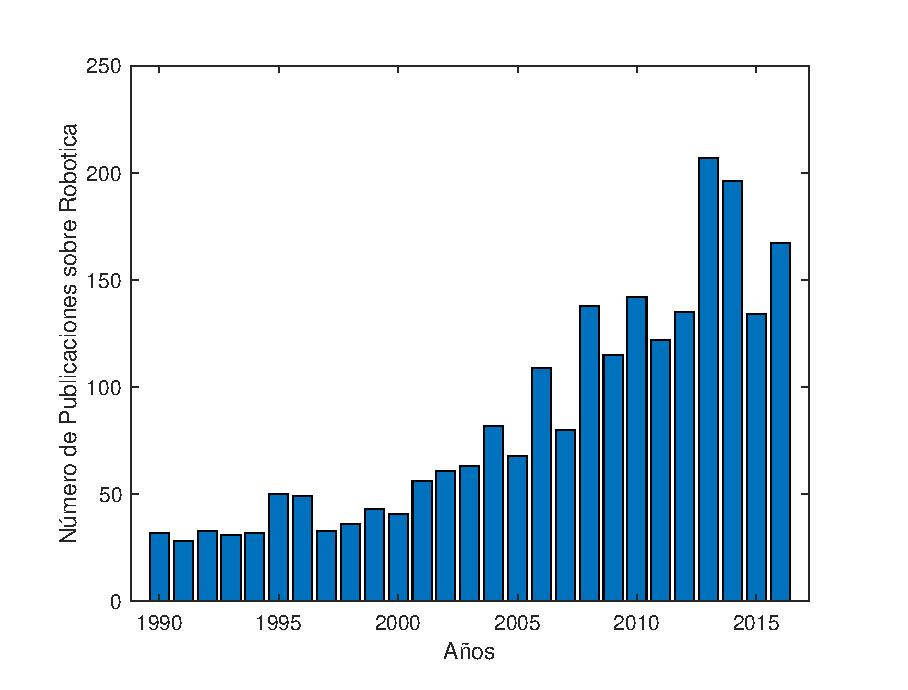
\includegraphics[width=0.7\textwidth]{Cap2_DisenoEspecificaciones/Figura/PublicacionesPorAnio.eps}
    \caption{Publicaciones por año}{Fuente:\citep{yuan2018review}}
    \label{fig:PublicacionesPorAnio}
\end{figure}

\subsubsection{Robot Herramienta Serial}

La industria de la robótica ha dejado a un lado los mecanismos convencionales para las máquinas herramientas, ver Figura \ref{fig:CartesianMachiningTool}, para utilizar una arquitectura serial, o de lazo abierto,  la cual consiste por una serie de eslabones unidos mediante juntas que permiten el movimiento relativo, ver Figura \ref{fig:MachiningSerialRobot}. Los primeras investigaciones sobre estos datan a inicios de los años 90’s, y desde entonces han sido intensamente investigado alrededor del mundo por su potencial de ser aplicado en distintos procesos de maquinado y manufactura \citep{chen2013robot}. Estas investigaciones abarcan temas como el diseño \citep{denkena2017design}, análisis de condición cinemática \citep{zargarbashi2012jacobian}, análisis de rigidez por su postura \citep{guo2015stiffness}, la utilización de redundancias [11], y el control de los mismo [12].

\begin{figure}[ht!]
    \centering
    \begin{subfigure}{0.45\textwidth}
        \centering
        \includegraphics[width=0.8\linewidth]{Cap2_DisenoEspecificaciones/Figura/CartesianMachiningTool.pdf}
        \caption{Máquina Herramienta Cartesiana}{Fuente:\citep{szipka2018measurement}}
        \label{fig:CartesianMachiningTool}
    \end{subfigure}
     \begin{subfigure}{0.45\textwidth}
        \centering
        \includegraphics[width=0.8\linewidth]{Cap2_DisenoEspecificaciones/Figura/MachiningSerialRobot.pdf}
        \caption{Robot Herramienta Serial}{Fuente:\citep{mejri2016dynamic}}
        \label{fig:MachiningSerialRobot}
    \end{subfigure}
    \caption{Comparación de Maquina herramienta y Robot herramienta}
\end{figure}

En el diseño de robot seriales, \cite{denkena2017design} en su trabajo \enquote{Design and optimization of a machining robot} explica que para los robots seriales presentan una serie de debilidades y limitaciones frente a las máquinas herramientas convencionales. Siendo que la principal limitación es la rigidez del robot, debido a que es inferior si es comparada con las máquinas convencionales, y es importante en la precisión de la trayectoria a seguir así como en la productividad del mismo. Por esto, los autores antes de realizar el diseño detallado y optimización del robot, realizan una evaluación cinemática de los conceptos de máquinas, mostrando que esta desventaja puede ser eliminada utilizando una cinemática adaptada con menor número de juntas, ver Figura \ref{fig:07ConceptEvaluation}.

\begin{figure}[ht!]
    \centering
    \includegraphics[width=0.8\textwidth]{Cap2_DisenoEspecificaciones/Figura/07ConceptEvaluation.pdf}
    \begin{tabular}[c]{p{0.2\textwidth} | m{0.2\textwidth} | m{0.2\textwidth} | m{0.2\textwidth} |}
         & Cinemática serial con solo juntas rotatorias & Cinemática serial guiada lineal & Cinemática serial con mesa lineal giratoria \\ \hline
        Rigidez & $\ominus$ & $\oplus$ &  $\oplus \oplus$ \\ \hline
        Modo Normal & $\ominus$ & $\oplus$ &  $\oplus \oplus$ \\ \hline
        Espacio & $\oplus$ & $\oplus$ & $\ominus$ \\ 
        de Instalación & & & \\ \hline
        Costo & $\oplus \oplus$ & $\oplus$ &  $\ominus \ominus$ \\ \hline
    \end{tabular}
    \caption{Conceptos de Robots seriales}{Fuente:\citep{denkena2017design}}
    \label{fig:07ConceptEvaluation}
\end{figure}

Por otra parte, en el análisis de condición cinemática, \cite{zargarbashi2012jacobian} en \enquote{The Jacobian condition number as a dexterity index in 6R machining robots} detalla sobre la utilización de un número de condición basado en el jacobiano como índice de desempeño. Teniendo en cuenta que este índice no tendría en cuenta los efectos dinámicos debido a las condiciones de trabajo durante el maquinado, siendo bajas velocidades, los efectos del husillo afectan la estructura y los altos modos de frecuencia del sistema. El número de condición trabaja teniendo en cuenta un pequeño error en las juntas, $\delta\dot\theta$, que produce un error en movimiento del efector, $\delta t$; recordando que las velocidades de estos elementos se relacionan a través de la matriz jacobiana, Ecuación \ref{Eq:IOVelocityEquation}, y que la inducción de este error en la posición, $\delta\theta$, afecta igualmente al jacobiano, $J\left(\theta + \delta\theta \right)$, sin embargo, puede ser aproximado de la siguiente manera $J\left(\theta + \delta\theta \right) \approx J\left(\theta\right)$. Por lo que los errores de velocidades pueden ser expresados por la Ecuación \ref{Eq:ErrorIOEquation}, simplificados de la forma Ecuación \ref{Eq:SimpleErrorIOEquation}, y en base a esto, el número de condición se obtiene relacionando la ecuación \ref{Eq:SimpleErrorIOEquation} con la ecuación \ref{Eq:IOVelocityEquation}, ver ecuaciones \ref{Eq:ConditionEquation} y \ref{Eq:ConditionExpression}. El número de condición manejaría valores entre $1$ y $\infty$, siendo que entre más pequeño el número de condición más uniforme será el cambio de las juntas sobre el efector.

\begin{subequations}
    \begin{eqnarray}
        \dot\theta = J^{-1}\left(\theta\right) t \label{Eq:IOVelocityEquation} \\
        \dot\theta + \delta\dot\theta = J^{-1}\left(\theta\right) \left(t + \delta t\right) \label{Eq:ErrorIOEquation} \\
        \delta\dot\theta = J^{-1}\left(\theta\right) \delta t \label{Eq:SimpleErrorIOEquation} \\
        \frac{\left\lVert \delta\dot\theta \right\rVert}{\left\lVert \dot\theta \right\rVert} \leq \kappa\left( J \right) \frac{\left\lVert \delta t \right\rVert}{\left\lVert t\right\rVert} \label{Eq:ConditionEquation} \\
        \kappa\left(J\right) = \left\lVert J\left(\theta\right) \right\rVert \cdot \left\lVert J^{-1}\left(\theta\right) \right\rVert \label{Eq:ConditionExpression}
    \end{eqnarray}
\end{subequations}

En el análisis de rigidez, el \cite{guo2015stiffness} y su artículo \enquote{Stiffness-oriented posture optimization in robotic machining applications} especifica un método optimización de postura de un robot serial que apunta a incrementar su rigidez, debido a que estos robots presentan múltiples soluciones para una posición del efector final \citep{zhu2013off}, como el ejemplo donde un robot de taladrado para un punto y dirección de un agujero no aplica una única pose, en la Figura \ref{fig:13OnePointTwoPoses} se muestra dos posibles poses del efector para taladrar un mismo agujero. Por eso, \cite{guo2015stiffness} mediante la utilización del modelo de rigidez del robot para seleccionar dentro de todas las poses posibles la que más óptima, es decir aquella que maximice la rigidez del sistema.

\begin{figure}[ht!]
    \centering
    \includegraphics[width=0.7\textwidth]{Cap2_DisenoEspecificaciones/Figura/13OnePointTwoPoses.pdf}
    \caption{Multipes poses para un mismo punto}{Fuente:\citep{zhu2013off}}
    \label{fig:13OnePointTwoPoses}
\end{figure}

En la implementación de redundancias, \cite{subrin2013new} para su investigación \enquote{New redundant architectures in machining: serial and parallel robots} evalua el desempeño de una arquitectura redundante de robot serial, observando como la implementación de lazo cerrado mejora el rendimiento cinemático como el rendimiento de rigidez de un manipulador serial.

Para la calibración y control de los robots seriales, \cite{andres2011calibration} en trabajo \enquote{Calibration and control of a redundant robotic workcell for milling tasks} detalla el procedimiento para la sintonización de un manipulador serial ${KUKA}^{TM}$, en donde propone un método para la calibración de este dispositivo en el sitio, usando sensores láser de desplazamiento y con una restricción de plano de no contacto. Estos procedimientos son sencillos de implementar y los recomienda para la mayoría de los robots industriales por su rapidez en el sitio.

En breve de los robots seriales, son mecanismos con una cadena cinemática abierta, la cuál le otorga un amplio espacio de trabajo, múltiples posturas para un misma posición y sencillez en el control, pero del mismo modo, produce baja estabilidad y rigidez en el sistema.

\subsubsection{Robot Herramienta Paralelo}
La creciente demanda de productos con mejores especificaciones ha llevado a la industria de la fabricación a incrementar los requerimientos y el rendimiento de los robots industriales, exigiendo mayores niveles de precisión operacional, capacidad de trabajo, confiabilidad y ciclo de vida. Una tendencia para la satisfacción de estas demandas radica en la implementación de manipuladores paralelos, los cuales poseen un potencial de trabajo alto, resaltando características como su alta rigidez, alta precisión y alta capacidad de carga \citep{zhang2009parallel}, además de ciertas ventajas como forma isotrópica, espacio libre de singularidades, rendimiento kinostatico uniforme y reconfigurabilidad \citep{lin2015design,ur2009kinematic,ZENG2014648}; por esto han sido implementado en la rehabilitación de brazo, mover y poner, maquinado de precisión o simulador de braquiterapia \citep{briot2009pantopteron,cardou2010dimensional,hoppner2015two,martini2015static}.

Por esto en la literatura se estudia a los mecanismos paralelos desde el análisis de una configuración \citep{sarabandi2018reconfigurable}, análisis cinemático \citep{gallardo2014application}, análisis dinámico \citep{xu2017dynamic}, el diseño \citep{li2018design}, Optimización \citep{kelaiaia2012multiobjective} y el control \citep{cazalilla2016hybrid}.

En el análisis de configuración, está el caso de \cite{sarabandi2018reconfigurable}, quien en su artículo \enquote{A Reconfigurable Asymmetric 3-UPU Parallel Robot} analiza la arquitectura UPU, \textit{Universal - Prismática - Universal}, por la posibilidad que tiene un mecanismo de tres brazos con esta arquitectura de presentar un movimiento puramente traslacional o puramente rotacional según su modo de ensamble. Esta configuración fue previamente estudiada por \cite{di1998translational}, quien determinó cuales son las condiciones que deben cumplir las universales, más específicamente el par de revolutas que la conforman, para producir movimientos de traslación; por otro lado, \cite{karouia2000three} estudio las condiciones constructivas que permiten un movimiento completamente rotacional en la plataforma. Sin embargo, el mecanismo presenta una sensibilidad a errores y zonas de su espacio de trabajo donde tiene un movimiento mixto,   traslación – rotación, y es por esto que los autores introducen una configuración asimétrica que permita prevenir estos inconvenientes de la arquitectura.

\begin{figure}
    \centering
    \begin{subfigure}{0.45\textwidth}
        \includegraphics[width=0.9\linewidth]{Cap2_DisenoEspecificaciones/Figura/Sarabandi2018-01.pdf}
        \caption{Mecanismo Traslacional}
        \label{fig:Sarabandi2018-01}
    \end{subfigure}
    \begin{subfigure}{0.45\textwidth}
        \includegraphics[width=0.8\linewidth]{Cap2_DisenoEspecificaciones/Figura/Sarabandi2018-02.pdf}
        \caption{Mecanismo Rotacional}
        \label{fig:Sarabandi2018-02}
    \end{subfigure}
    \caption{Arquitectura propuesta por \cite{sarabandi2018reconfigurable}}
    \label{fig:Sarabandi2018}
\end{figure}

En el análisis cinemático, \cite{gallardo2014application} en su trabajo \enquote{An application of screw theory to the kinematic analysis of a Delta-type robot} detalla los pasos de un análisis cinemático para un mecanismo tipo delta, ver Figura \ref{fig:Gallardo2014}, explicando el método por \citep{pierrot1990delta} para resolver el problema de cinemática inversa de este; para después realizar el análisis de velocidades aplicando teoría de tornillo, un recurso matemático que hace uso de las coordenadas de Plücker para simbolizar el estado de movimiento de cada revoluta además de la forma de Klein de la algebra de Lie para calcular las velocidades; por último, el análisis de aceleración aplica la misma teoría; los resultados son verificados con un software de simulación llamado ADAMS.

\begin{figure}[htb!]
    \centering
    \includegraphics[width=0.5\textwidth]{Cap2_DisenoEspecificaciones/Figura/Gallardo2014.pdf}
    \caption{Robot delta simulado en ADAMS}{Fuente: \citep{gallardo2014application}}
    \label{fig:Gallardo2014}
\end{figure}

En el análisis dinámico, \cite{xu2017dynamic} explica, en \enquote{Dynamic analysis of a linear Delta robot in hybrid polishing machine based on the principle of virtual work}, un método llamado trabajo virtual para resolver el análisis dinámico de un robot delta lineal, ver Figura \ref{fig:Xu2017}; dicho método apunta a resolver las fuerzas motrices de las juntas prismáticas, teniendo en cuenta las fuerzas y momentos inerciales de cada cuerpo móvil alrededor del punto de pivote. Por otro lado, esta metodología recibe su nombre debido a que se supone un desplazamiento virtual, interrelacionando los desplazamientos de cada cuerpo con las entradas a través de matrices jacobianas, con esto se calcula los trabajos realizados por todas las fuerzas externas del mecanismo, y por último, se determinan las fuerzas de los actuadores.

\begin{figure}[hbt!]
    \centering
    \includegraphics[width=0.4\textwidth]{Cap2_DisenoEspecificaciones/Figura/Xu2017.pdf}
    \caption{Modelo 3D del robot paralelo}{Fuente: \citep{xu2017dynamic}}
    \label{fig:Xu2017}
\end{figure}

En el diseño, \cite{li2018design} trabaja el diseño de un robot paralelo con configuración 3-CPS, esto lo hace en el artículo \enquote{The design of a 3-CPS parallel robot for maximum dexterity}. En la primera etapa del diseño se selecciona la arquitectura con la que se va a trabajar, especificando sus ventajas y desventajas, para su caso escogieron los SDelta, ver Figura \ref{fig:Li2018}, debido a que son robots paralelos con 6 grados de libertad, esto implementando 3 brazos, de ahí que eviten interferencia entre los brazos, así como baja carga inercial. Además todos sus motores están ubicados en la base. Luego de esto, el procedimiento de diseño continúa con los análisis cinemáticos y cinéticos, determinando la cinemática inversa o la directa, un análisis de singularidades y por último, un análisis de fuerzas. Esto es hecho para mirar el comportamiento del mecanismo ante una medidas determinadas. El diseño prosigue con una optimización dimensional, la cual se hace es llevada a cabo midiendo un índice de desempeño. Este índice o conjunto de índice son escogidos en función de los requerimientos de la aplicación.

\begin{figure}[hbt!]
    \centering
    \includegraphics[width=0.5\textwidth]{Cap2_DisenoEspecificaciones/Figura/Li2018.pdf}
    \caption{Arquitectura SDelta}{Fuente: \citep{li2018design}}
    \label{fig:Li2018}
\end{figure}

En la Optimización, \cite{kelaiaia2012multiobjective} en su trabajo \enquote{Multiobjective optimization of a linear Delta parallel robot} muestra como la síntesis dimensional es vital para el buen diseño de un robot paralelo. Propone una metodología para este problema, ver Figura \ref{fig:Kelaiaia2012}, el cual es expresado en términos de una optimización multiobjetivos teniendo en cuenta varios criterios de rendimiento. Dichos criterios de evaluación miden el rendimiento del espacio de trabajo, la rigidez, así como el comportamiento cinemático y dinámico. Para llevar a cabo la optimización utilizan un algoritmo genético SPEA-II, configurado con 200 miembros de la población, 200 generaciones, 90\% de probabilidad de cruzamiento y probabilidad de mutación del 10\%.

\begin{figure}[hbt!]
    \centering
    \includegraphics[width=0.5\textwidth]{Cap2_DisenoEspecificaciones/Figura/Kelaiaia2012.pdf}
    \caption{Metodología propuesta}{Fuente: \citep{kelaiaia2012multiobjective}}
    \label{fig:Kelaiaia2012}
\end{figure}

En breve, los robots paralelos presentan una serie de ventajas cinemáticas y dinámicas, comparados con las otras dos tecnologías. Para aprovechar estas ventajas en la etapa de diseño, se deben analizar desde la arquitectura, pasando por cada uno de los análisis cinemáticos y cinéticos, así como otros necesarios para los criterios de la aplicación, hasta la parte de la síntesis dimensional del mecanismo.

\begin{center}
    \begin{longtable}{>{\columncolor[gray]{0.85}} p{0.3\textwidth} p{0.3\textwidth} p{0.3\textwidth} }
        \rowcolor[gray]{0.85}
         & \centering \textbf{Comparativo de las arquitectura}  & \\   \hline
        \textbf{Caracteristicas} & \textbf{Serial} & \textbf{Paralela} \\
        \endfirsthead \hline
        \textbf{Caracteristicas} & \textbf{Serial} & \textbf{Paralela} \\ \hline \endhead \hline 
        Cinemática & \Large $\star\star\star\star\star$ & \Large $\star\star$ \\
         & Simple & Compleja \\ \hline
        Capacidad Dinamica & \Large $\star\star\star$ & \Large $\star\star\star\star\star$ \\
         & Limitada & Elevada \\ \hline
        Rigidez & \Large $\star\star$ & \Large $\star\star\star\star\star$ \\
         & Pobre & Elevado \\ \hline
        Destreza & \Large $\star\star\star\star\star$ & \Large $\star\star\star$ \\
         & Excelente & Alto \\ \hline
        Control & \Large $\star\star\star\star\star$ & \Large $\star\star$ \\
         & Simple & Compleja \\ \hline
        Modularidad & \Large $\star\star\star$ & \Large $\star\star\star\star\star$ \\
         & Alto & Excelente \\ \hline
        \caption{Resumen del estado de los robots}
        \label{table:ResumenEstadodelArteMecanismo}
    \end{longtable}
\end{center}

%%%%%   Estado de la Técnica    %%%%%
\subsection{Estado de la Técnica}

En la industria actual existe una amplia oferta de equipos para llevar a cabo procesos de fabricación de piezas de alta calidad como el maquinado. En cuanto al proceso de fresado existen 3 tipos de soluciones comerciales actuales muy competitivas en el mercado.

\begin{longtable}[c]{m{0.5\textwidth} m{0.05\textwidth} m{0.35\textwidth}}
    \hline \rowcolor[gray]{0.9} \textbf{EUROPA} & & \\ \hline
    \textbf{Empresas} & \textbf{Ejes} & \textbf{Aplicación} \\
    Demaurex/Delta          & 3 & Manipulador \\
    PKMtricept SL           & 5 & Maquinado, Ensamblaje \\
    %Geodetics               & 6 & Maquinado \\
    Carl Zeiss Jena, Physik Instrumente         & 6 & Posicionamiento \\
    %Physik, Instrumente     & 6 & Posicionamiento \\
    %CMW                     & 6 & Maquinado \\
    Lapic Company           & 6 & Medición de coordenadas \\
    Fooke (Triomax)         & 3 & Corte agua/láser \\
    Urane SX (Renault)      & 3 & Taladrado de alta velocidad \\
    %Simparalell (Simplex), Starrag Group (Ecospeed 20210), Teknodrom (XT 1100S)   & 5 & Maquinado \\
    %Starrag Group (Ecospeed 20210) & 5 & Maquinado \\
    %Teknodrom (XT 1100S)    & 5 & Maquinado \\
    \textbf{Universidad-empresa} & & \\
    WZL Aachen – Ingersoll  & 6 & Maquinado \\
    %FhG Chemnitz – Mikromat & 5 & Maquinado \\
    IfW Stuttgart – INA (Hexact) & 5 & Maquinado \\
    ETH Zurich – Mikron (Triaglide) & 3 & Maquinado \\
    \textbf{Universidades} & & \\
    ISW Stuttgart (Linapod) & 3 & Maquinado \\
    IWF – Hannover          & 3 & Maquinado láser\\
    ETH Zurich (Hexaglide), ITIA – CNR (Acrobat)  & 6 & Maquinado \\
    %ITIA – CNR (Acrobat)    & 6 & Maquinado \\
    \hline \rowcolor[gray]{0.9} \textbf{ESTADOS UNIDOS} & & \\ \hline
    \textbf{Empresa} & & \\
    Tornado 2000 (Hexel), Rotapod (Hexel), Variax (Giddings and Lewis)    & 6 & Maquinado \\
    %Rotapod (Hexel)         & 6 & Maquinado \\
    %Variax (Giddings and Lewis) & 6 & Maquinado \\
    \hline \rowcolor[gray]{0.9} \textbf{ASIA} & & \\ \hline
    \textbf{Universidad-empresa} & & \\
    Eclipse – Universidad de Seul, Leadwell (X-700R), Okuma, HexaM & 6 & Maquinado \\
    %Leadwell (X-700R)       & 6 & Maquinado \\
    %Okuma                   & 6 & Maquinado \\
    %HexaM                   & 6 & Maquinado \\
    Honda Engineering       & 3 & Maquinado \\
    Fanuc Robotics (F-200i) & 6 & Soldadura \\ \hline
    \caption{Empresas fabricantes de maquinas herramientas}{Fuente: \citep{serje2017parallel}}
\end{longtable}
En los últimos años han surgido diversas iniciativas investigativas y propuestas sobre la aplicación de robots con arquitecturas paralelas como solución a ciertas limitaciones de las máquinas herramientas seriales. Algunos de estos diseños se han logrado comercializar ofreciendo mejoras en las capacidades dinámicas y rigidez de las máquinas herramientas entrando a la competencia de la industria de la fabricación y a su vez presentando nuevos retos de diseño y control. En la siguiente tabla se presentan algunas de las maquinas herramientas fabricadas hasta la fecha y las aplicaciones que estas han tenido.

~



\begin{longtable}{|>{\columncolor[gray]{0.85}}p{0.16\textwidth}|p{0.16\textwidth}|p{0.16\textwidth}|p{0.12\textwidth}|p{0.18\textwidth}|p{0.1\textwidth}|}
    \hline \rowcolor[gray]{0.85}
    \textbf{Fabricante} & \textbf{Modelo} & \textbf{Arquitectura} & \textbf{Velocidad} $\left[ m/min \right]$ & \textbf{ET} $\left[ mm \right]$  & \textbf{ET/VM} $\left[ \% \right]$ \\ \hline \endhead
    
    CharlyRobot  & Charly4U     & Paralela & 6     & 310x220x160   & --\\\cline{1-6}
    Chiron       & V-Concept    & Hibrida  & 120   & 450x300x300   & 2.77\\ \cline{1-6}
    DMG mori     & CMX600 V     & Cartesiana & 30  & 600x560x510   & 1.07\\ 
                 & CMX800 V     & Cartesiana & 30  & 800x560x510   & 0.82\\ 
                 & CMX1100 V    & Cartesiana & 30  & 1100x560x510  & 0.95\\\cline{1-6}
    Fatronik     & Ulyses       & Paralela & 50    & 500x500x500   & --\\ \cline{1-6}
    Hass         & VF-1         & Serial   & 16.5  & 508x406x508   & 0.63\\ 
    Automation   & Minimill2    & Serial   & 15.2  & 508x406x356   & 0.55\\ 
                 & OM-1A        & Serial   & 19.2  & 203x203x305   & 0.52\\\cline{1-6}
    Heckert      & SKM400       & Paralela & 100   & 630x630x630   & --\\ \cline{1-6}
    Hitachi Seiki & PA35II      & Paralela & 100   & 350x350x200   & --\\ \cline{1-6}
    Honda        & HVS500       & Hibrida  & 60    & 650x500x400   & --\\ \cline{1-6}
    HullerHille  & Specht-      & Hibrida  & 120   & 630x630x750   & --\\ 
                 & Xperimental  &          &       &               &   \\ \cline{1-6}
    Index        & V100         & Paralela & 50    & 280x280x145   & 0.09\\ \cline{1-6}
    ISWstuttgart & Linapod      & Paralela & 45    & 400x400x400   & 0.46\\ \cline{1-6}
    IRCCyN       & Orthoglide   & Paralela & 100   & 200x200x200   & 0.46\\ \cline{1-6}
    JSWAY        & JDV850       & Paralela & 10    & 800x500x500   & 1.04\\ \cline{1-6}
    Krauseco     & QuickStep    & Paralela & 80    & 630x630x500   & --\\ 
     Mauser      & HS500        &          &       &               &    \\ \cline{1-6}
    Leadwell CNC & V-20i        & Cartesiana &       & 510x350x400   & --\\
    Machines     & V-30         & Cartesiana &       & 600x400x300   & --\\ \cline{1-6}
    Light        & Spectra      & serial   & 0.76  & 216x114x140   & 1.73\\
    Machines Corp & light200    &          &       &               &   \\ \cline{1-6}
    Mazak        & VC-300A      & Paralela & 24    & 350x300x305   & 0.50\\ 
                 & VC-500C      & Paralela & 30    & 500x1000x510  & 0.07\\ 
                 & VC-500A/2PC  & Paralela & 30    & 505x505x510   & 4.70\\ \cline{1-6}
    Mikron       & Triaglide    & Paralela &       & 170x120x250   & 0.16\\ \cline{1-6}
    OKuma        & MB-46V       & Paralela & 32    & 500x460x460   & 0.75\\ 
                 & MB-500H      & Paralela & 60    & 500x500x460   & 0.28\\ \cline{1-6}
    Sharp        & LMV-50       & Paralela &       & 812,279x127   & 4.25\\ 
                 & TMV          & Paralela &       & 711x381x127   & 2.14\\ 
                 & LMV          & Paralela &       & 635x279x127   & 3.83\\\cline{1-6}
   Techno Inc    & RG5950       & Paralela & 20.32 & 1500x1300x254 & 6.58\\ \cline{1-6} 
   Mikron        & Triaglide    & Paralela &       & 170x120x250   & 0.16\\ \cline{1-6}
   University    & LOLA         & Paralela & 10    & 120x100x35    & 0.35\\ 
   of Belgrade   &              &          &       &               &   \\ \cline{1-6}
   WZL Aachen    & DynaM        & Hibrida  & 90    & 630x630x500   & 2.21\\ \cline{1-6}
                 
                            
    \caption{ Máquinas Fresadoras de 3 ejes actuales}{Fuente: Elaboración propia}
\end{longtable}
La tabla anterior realiza una comparativa de algunas especificaciones de fresadoras de 3 ejes abarcando una amplia gama de capacidades, distintos fabricantes y arquitecturas. Como resultado de esta encontramos velocidades lineales promedio de 45m/min para espacios de trabajo de 550x450x370 mm con una compacidad de la máquina de 1.5\%. La tabla es resultado de elaboración propia con adaptaciones de \cite{serje2017parallel}.


%\begin{figure}[ht!]
%    \centering
%    \includegraphics[width = 0.5\textwidth]{Cap2_DisenoEspecificaciones/Figura/Perfect-Jet_MCV-M8.pdf}
%    \caption{Máquina Herramienta de Perfect-jet}
%    \label{fig:Perfect_jet-MCV-M8}
%\end{figure}

\subsection{Revisión de Patentes}
En la parte de patentes sobre máquinas herramientas se ha encontrado distintas tecnologías aplicadas como los son manipuladores paralelos, robots serial y cartesianos, además de mecanismos híbridos entre seriales y paralelos. Estas patentes son mostradas a continuación en detalle, y al final serán resumida en la tabla \ref{table:PatentRevision}.

\textbf{CN109676587A} - \textit{A kind of four-degree-of-freedom high speed parallel robot} \citep{patent:CN109676587A}: La patente proporciona un robot paralelo de alta velocidad de cuatro grados de liberta. Este este compuesto por una base, una plataforma de movimiento, efector final, cuatro cadenas de ramificación. La plataforma de movimiento está compuesta por una plataforma superior, una inferior un acople giratorio y un mecanismo amplificador de ángulo. este mecanismo amplificador de ángulo está dispuesto entre la plataforma inferior y la superior. Se utilizan juntas esféricas y giratorias.

\textbf{AU2007297702B2} - \textit{Systems, devices, and methods for surgery on a hollow anatomically suspended organ.} \citep{patent:AU2007297702B2}: La patente expone un dispositivo (Robot) para el uso de operaciones microquirurgicas (ocular), El dispositivo posee un robot híbrido esclavo que tiene al menos dos brazos robóticos (cada brazo robótico tiene un robot en serie conectado a un robot paralelo) y un maestro tele-robótico que tiene al menos dos esclavos maestros controlados por el usuario interfaces ( joysticks). 

\textbf{WO2019091425A1} - \textit{Few-joint over-constrained five-freedom-degree hybrid connection robot} \citep{patent:WO2019091425A1}: La patente aporta un robot con una conexión hibrida de pocas articulaciones con cinco grados de libertad, ver Figura \ref{fig:WO2019091425A1}. Este está compuesto por: una plataforma fija (11), marcos verticales de tipo erecto (10), un marco de rotación de par de rotación simple (8), doble marco de rotación de par de rotación (6), una plataforma móvil (3), una plataforma de trabajo (1), tres cadenas de ramificación (4,5, 9) de una misma estructura y un cabezal de ajuste de postura de dos grados de libertad (2).

\begin{figure}[ht!]
    \centering
    \includegraphics[width = 0.5\textwidth]{Cap2_DisenoEspecificaciones/Figura/WO2019091425A1.pdf}
    \caption{Robot de 5-GDL conexión hibrida}{Fuente:\citep{patent:WO2019091425A1}}
    \label{fig:WO2019091425A1}
\end{figure}

\textbf{CN109091233A} - \textit{Puncturing operation robot based on series and parallel structure} \citep{patent:CN109091233A}: Esta patente pertenece al campo técnica de los dispositivos médicos, es un robot para cirugía de punción basado en una estructura en serie-paralela. La máquina está compuesta de una base, un mecanismo de ajuste y postura y un mecanismo de inserción de aguja. Las acciones del robot de cirugía de punción del control atreves de los cinco grados de libertad de la estructura serie- paralela.

\textbf{ES2433664T3} - \textit{Dispositivo guiador dirigible} \citep{patent:ES2433664T3}: Esta patente presenta una sonda robótica articulada, con 2 mecanismo que pueden operar coordinados o según la configuración que se necesite, flácido o rígido.

\textbf{US5715729A} - \textit{Machine tool having parallel structure} \citep{patent:US5715729A}: Trata del diseño de un robot paralelo con seis grados de libertad, Figura \ref{fig:US5715729A}, con 6 brazos y 6 motores, una placa base fija y una sección móvil, destinado a trabajar materiales duros y a un enfoque industrial.

\begin{figure}[ht]
    \centering
    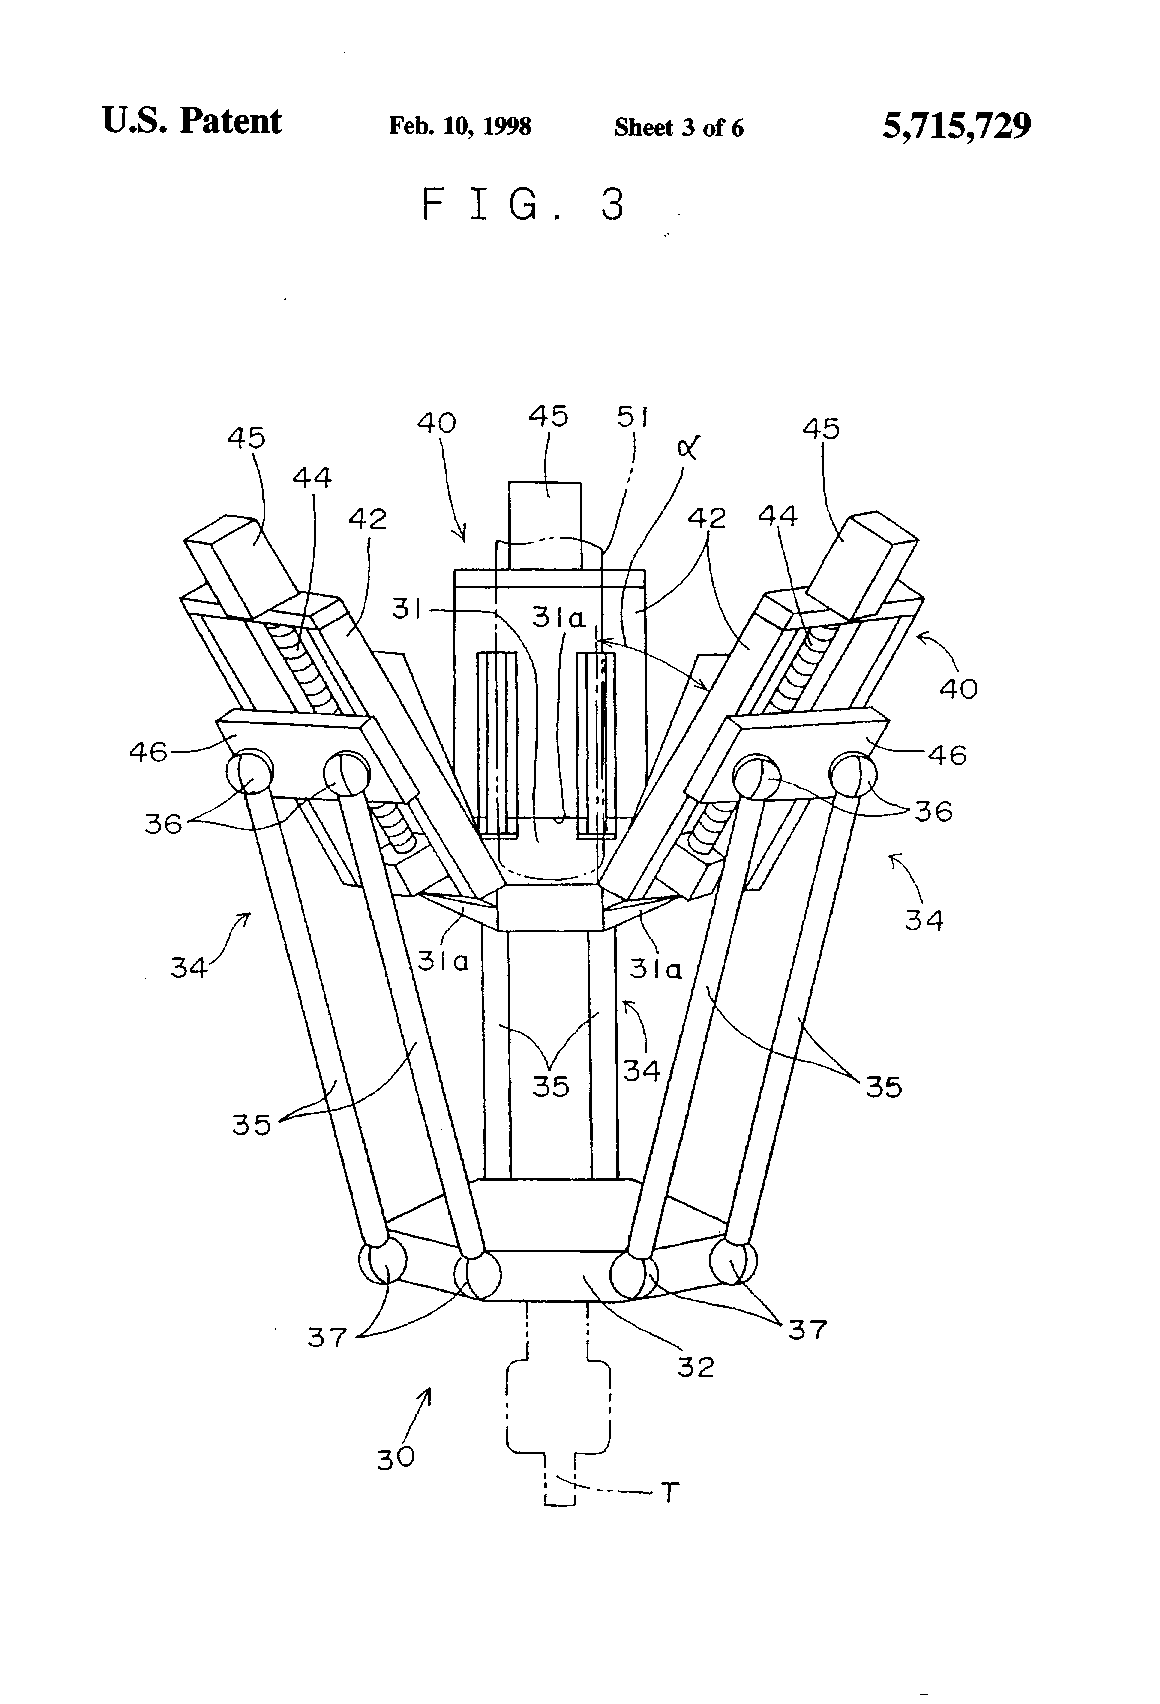
\includegraphics[width = 0.5\textwidth ]{Cap2_DisenoEspecificaciones/Figura/US5715729A.pdf}
    \caption{Estructura para máquina paralela}{Fuente:\citep{patent:US5715729A}}
    \label{fig:US5715729A}
\end{figure}

\textbf{ES2392059B2} - \textit{Robot de estructura cinemática híbrida para el guiado de la inserción de agujas, catéteres y elementos quirúrgicos para procedimientos de cirugía mínimamente invasiva.} \citep{patent:ES2392059B2}: 

\textbf{CN109348795A} - \textit{A kind of replanting system and its implementation based on parallel robot} \citep{patent:CN109348795A}: La invención describe con un sistema de transporte basado en un robot paralelo y un método de implementación del sistema. EL sistema está compuesto por Una estructura de marco, robot paralelo y un dispositivo de transporte.

\textbf{US 8,776,632 B2} - \textit{Actuación de baja carrera para un robot en serie.} \: 


%\textbf{CN201579788U} - \textit{Opened field type six-freedom-degree serial-parallel processing robot}: La patente es de un robot serie-paralelo de seis grados de libertad (campo abierto) que cuenta con sensores de fuerza, cámara de visión que envían información a un controlador que calcula donde está el husillo y la fuerza para moverlo.
~
\definecolor{Gray}{gray}{0.85}
\begin{longtable}{|>{\columncolor[gray]{0.85}}p{0.25\textwidth}|p{0.4\textwidth}|p{0.33\textwidth}|}
\hline \rowcolor[gray]{0.85}
\textbf{\large Patente} & \textbf{\large Ventajas} & \textbf{\large Desventajas} \\ \hline \endhead
CN109676587A & Fuerzas de fricción pequeñas entre los accesorios. & \\
 & Se puede ajustar el coeficiente de amplificación de ángulo. & Volumen de la máquina. \\
 & Cadenas de ramificación simples. & \\ \cline{1-3}
 
ES2588015 & Gran espacio de trabajo, & Baja compacticidad \\
 & logra realizar geometrias muy complejas. & ,Necesita una base giratoria. \\ \cline{1-3}
 
WO2019091425A1 & Una mejora en la rigidez integral de la estructura. & \\
 & Reducción en la dificultad de control. & \\
 & Análisis cinemático es simple y respuesta dinámica buena. & \\
 & Por la combinación de cabezal oscilante de dos grados de libre la plataforma móvil, se amplía el espacio de trabajo de una máquina de herramienta. & \\ \cline{1-3}
 
ES2392059B2 & Mecanismo hibrido, Diseño modular, 6 grados de libertad, Sistema hibrido, bajo peso, cuenta con un sistema guiado por laser. & Sistema de control complejo, estructura ligeramente debil.\\
 & . & \\ \cline{1-3}
 
CN109091233A & La operación de ajuste y postura de la aguja se pueden completar automáticamente. & Un tamaño pequeño conveniente para el uso médico, pero no para el uso industrial \\
 & Una estructura simple en general. &  \\ \cline{1-3}

ES2433664T3 & Puede ser utilizado en multiples campos por su adaptibilidad. Se pueden adaptar camaras, medicamentos entre otros al interior del dispositivo, es muy flesible. Ideal para espacios reducidos (Tuberias). & Solo maneja 3 ejes, maneja bajas cargas, se necesitan una gran cantidad de sensores y controladores para operar correctamente. Se hace necesario la sincronizacion del mecanismo interno con el externo.
  \\ \cline{1-3}

US5715729A & Trabajo con grandes cargas, sistema de control "sencillo" & \\ \cline{1-3}

AU2007297702B2 & Altamente preciso, portable, cuenta con herrramientas modulares. & Espacio de trabajo reducido, se debe de tener en cuenta las posibles singularidades, en funcion de su area de trabajo, es poco compacto.\\ \cline{1-3}

US8776632B2 & Sistema de control "sencillo", liviano, bajo costo. & Trabaja con bajas cargas, rango de movilidad limitado. \\ \cline{1-3}

CN109348795A & Mejora de la eficiencia enormemente. & \\
 & El sistema es más liviano. & \\
 & Una estructura simple y es más conveniente para la operación en comparación de un robot serie. & \\ \cline{1-3}
 
%CN201579788U & Compacta & \\
% & Económica & \\
% & Alta Precisión & \\ \cline{1-3}
\caption{Revisión de Patentes}{Fuente: Elaboración Propía}
\label{table:PatentRevision}
\end{longtable}
%\newpage
%%%%%   Definición de Especificaciones    %%%%%
\section{Definición de Especificaciones}
\subsection{Despliegue de Función de Calidad (QFD)}

La matriz QFD es una parte fundamental del proceso de diseño que facilita la generación de especificaciones de el producto o maquina a fabricar, permite hacer una comparación entre las caracteristicas que intervienen en este teniendo en consideracion los requerimientos del cliente y de diseño. La matriz QFD presenta de manera resuminda y confronta las caracteristicas requeridas, los pros y contras, de manera que se traduzcan tales requerimientos en variables de ingenieria (medibles) y de este modo facilitar la toma de desciciones y la propuesta de alternativas.

\begin{landscape}
\begin{figure}[hb!]
    \centering
    \includegraphics[scale=0.9]{Cap2_DisenoEspecificaciones/Figura/QFD.pdf}
    \caption{QFD}
    \label{fig:QFD}
\end{figure}
\end{landscape}

\subsection{Listado de referencia de especificaciones}

La lista de referencia es una estrategia de diseño que busca desarrollar una lista de especificaciones iniciales suficientes, las cuales se construyen a partir de los estudios del estado del arte, estado de la tecnica y analisis del QFD donde se intenten abordar todos los aspectos y elementos del diseño y apuntar a la obtencion de especificaciones completas. 
\begin{longtable}{|>{\columncolor[gray]{0.85}}p{0.25\textwidth}|p{0.70\textwidth}|}
    \cline{1-2} \rowcolor[gray]{0.85}
    \textbf{Concepto} & \textbf{Determinaciones } \\ \hline \endhead
    Funcion     & Descripcion de las funciones principales, ocasionales y accidentales del producto.\\ \cline{1-2}
    Dimensión   & Espacios, Volumenes, masas, longitudes, alturas, anchuras, diametros; numero y disposicion de elementos \\ \cline{1-2}
    Movimientos & Tipos de movimiento; desplazamientos, secuencias y tiempos; trayectorias, velocidades y aceleraciones.\\ \cline{1-2}
    Fuerzas     & Magnitud, direccion y sentido de fuerzas y momentos; variacion en el tiempo; desequilibrios y deformaciones admisibles.\\ \cline{1-2}
    Energia     & Accionamientos mecanico y otros conversores de energia: alimentacion y control; transmisiones; potencia y rendimiento.\\ \cline{1-2}
    Materiales  & Flujo, transporte y transformacion de materiales; limitaciones o preferencias sobre su uso; condicionantes de mercado.\\ \cline{1-2}
    Señales y control & Señales de entrada y salida; sensores y actuadores; funciones del sistema de control.\\ \cline{1-2}
    Fabricacion y montaje & Volumen previsto de produccion y cadencia en el tiempo; limitaciones o preferencias en procesos y equipamientos; variantes en el producto de flexibilidad en la fabricacion.\\ \cline{1-2}
    Transporte y distribucion & Embalaje y transporte: dimensiones, masas, orientacion, golpes; instalacion, montaje y puesta a punto.\\ \cline{1-2}
    Vida util y Mantenimiento & Vida prevista; fiabilidad y mantenibilidad; tipo de mantenimiento e intervalos de servicio; criterios sobre recambios.\\ \cline{1-2}
    Costes y plazos & Costes de desarrollo y preparacion de utillaje; plazos de desarrollo y tiempo para el mercado.\\ \cline{1-2}
    Seguridad y ergonomía & Sistemas y dispositivos de seguridad; relacion con el usuario; operacion, inteligibilidad, confort y aspecto.\\ \cline{1-2}
    Impacto ambiental & Consumos de energía y materiales; limitaciones al impacto ambiental en la fabricacion, utilizacion y fin de vida.\\ \cline{1-2}
    Apectos legales & Cumplimiento de noremativas (Funcion de los usos y mercados); evitar la colision con patentes.\\ \cline{1-2}
    
    
    \caption{Lista de referencia de especificaciones}{Fuente: \cite{Riba2002}}
\end{longtable}
~
La tabla mostrada es el modelo de lista de referencia del método MEPEIS y se utilizó para la construcción del listado de referencia propio.
\begin{longtable}{|>{\columncolor[gray]{0.85}}p{0.25\textwidth}|c|p{0.60\textwidth}|}
    \cline{1-3} \rowcolor[gray]{0.85}
    \textbf{Concepto} & \textbf{R/D} & \textbf{Descripcion } \\ \hline \endhead
    Dimensión   & R & Relación Espacio de Trabajo/Volumen de la Máquina superior a $1,3\%$ \\
                & D & Espacio de Trabajo superior a $500\times 500\times 500$ mm \\ \cline{1-3}
    Movimientos & D & Entradas  paralelas \\
                & R & Presicion de 0.005 mm \\ \cline{1-3}
    Fuerzas     & R & Disminución de par requerido \\ \cline{1-3}
    Energía     & R & Ahorro Energético de los motores \\ \cline{1-3}
    Materiales  & R & Rigidez (Vibraciones) \\
                & R & Resistencia a Fatiga \\ \cline{1-3}
    Señales y Control   & R & RPM \\
                        & R & Velocidad de avance \\
                        & D & Aceleraciones \\
                        & R & Posición \\
                        & D & Torque \\ \cline{1-3}
    Vida Útil y Mantenimiento & D & Vida útil mayor a 10 años \\ \cline{1-3}
    Fabricación y Montaje   & D & Fabricación con piezas estándares y montaje modular \\
                            & D & Fácil remplazo de piezas dañadas, sea por la facilidad de comercialización (piezas estándar) o la capacidad de fabricar las mismas \\
                            & D & Facil mantenimiento por diseño moludar\\ \cline{1-3}
    Costos de Fabricación   & D & Costos de Fabricación inferiores a 40 Millones de pesos \\ \cline{1-3}
    Seguridad               & R & Alta protecion al operario \\
                            & R & Protecciones Electricas y Termicas de la maquina \\
    \cline{1-3}
    \caption{Requerimientos para Máquina CNC de 3 ejes}{Fuente: Elaboración propia}
\end{longtable}

\section{Normas}
\begin{center}
    \begin{longtable}{|>{\columncolor[gray]{0.85}} p{0.2\textwidth}| p{0.2\textwidth}| p{0.5\textwidth}| }
    \rowcolor[gray]{0.85} \hline
    \textbf{Estandar} & \textbf{Norma} & \textbf{Titulo}  \\ \hline \endhead
        {CEN} & TC 143      & Standardization in the field of safety of machine tools, their accessories and tools designed to form and to machine cold metal both with and without the removal of metal. \\ \hline
        {ISO} & 230-2       & Determination of accuracy and repeatability of positioning of numerically controlled axes. \\ \hline
        {ISO} & TR 230-8    & Test code for machine tools-Vibrations. \\ \hline
        {ISO} & 3685        & Tool-life testing with single-point turning tools. \\ \hline
        {ISO} & 1985        & Machine tools-Test conditions for surface grinding machines with vertical grinding wheel spindle and reciprocating table-Testing of accuracy.\\ \hline
        {ISO} & 230-3       & Determination of thermal effects. \\ \hline
        {ISO} & 8373       & Manipulating industrial robots.\\ \hline
        {ISO} & 9409-2       & Manipulación de robots industriales. Interfaces mecánicas. Parte 2: Ejes.\\ \hline
        
        \caption{Normas a utilizar}{Fuente: Elaboración Propia}
        \label{table:Normas}
       \end{longtable}
\end{center}
    
    %%%%%   Capitulo 3 : Diseño Conceptual    %%%%%
    %%%%%   Capitulo 3 : Diseño Conceptual    %%%%%
\chapter{Diseño Conceptual}

%%%%%   Metodología del Diseño Conceptual    %%%%%
\section{Metodología del Diseño Conceptual}
En el apartado del diseño de la solución esta presenta la fase conceptual, en donde el diseño está más enfocado en la generación y selección de conceptos de solución. Esta fase se caracteriza por tener presentar diferentes metodologías o maneras de generar alternativas, así como de evaluar estas. Algunos ejemplos de estas metodologías de generación de alternativas están presentes en el libro de \cite{dieter2012engineering}, donde explica métodos creativos como la lluvia de ideas, la sinéctica y el diseño biomimetico, así como métodos sistemáticos como la descomposición y síntesis funcional, el análisis morfológico y la teoría de la resolución inventiva de problemas (conocida como TRIZ por sus siglas en ruso). Por otro lado, en las metodologías de evaluación, \cite{dieter2012engineering} muestra los métodos sistemáticos de evaluación por medio de matrices de decisión, determinado por criterios ponderados, y en los cuales se destaca la Asignación Directa, el Árbol de Objetivos y el Proceso Analítico de Jerarquía (AHP por sus siglas en ingles).

Para este proyecto se hará de la metodología sistemática tanto para la generación como la evaluación de alternativas de diseño. En el parte de la generación se hará uso de la descomposición y síntesis funcional, así como del análisis morfológico; mientras que en la evaluación se hará uso del método AHP. Estos serán dispuestos de la siguiente manera:

\begin{enumerate} \nosep
    \item Descomposición y Síntesis Funcional.
    \item Definición y ponderación de criterios de selección
    \item Selección de tecnología de maquina herramientas
    \item Análisis morfológico.
    \item Generación de Alternativas.
    \item Proceso Analítico de Jerarquía  (AHP).
\end{enumerate}

%%%%%   Descomposición y Síntesis Funcional    %%%%%
\section{Descomposición y Síntesis Funcional del Sistema}
Este método de diseño conceptual, la descomposición y síntesis funcional, se basa en la estrategia común de descomponer un sistema complejo en unidades más sencillas que describan lo describan significativamente. Esta descomposición, además de ser obvia para el equipo desarrollador, debe reflejar ciertas agrupaciones naturales que comprenden una entidad o que sean mutuamente acordados por los usuarios. Por otra parte, este procedimiento es útil para comprender la tarea de diseño y asignarle recursos \citep{dieter2012engineering}. 

Basado en lo descrito por \cite{dieter2012engineering}, este método consta de 3 partes, una Descomposición Física, una Representación Funcional (o Despliegue de Funciones) y una Estructura Funcional (o Análisis Funcional).

Para este proyecto se llevará a cabo el Despliegue de Funciones (ver Sec. \ref{sec:DespliguedeFunciones}) y el Análisis Funcional (ver Sec. \ref{sec:AnalisisFuncional}).

%%%%%   Despliegue de Funciones    %%%%%
\subsection{Despliegue de Funciones}
\label{sec:DespliguedeFunciones}

El despliegue de funciones consiste de una descomposición del sistema a diseñar, partiendo desde la función global del dispositivo, pasando por cada una de las funciones que debe llevar a cabo y finalizando en las subfunciones necesarias. Con estos tres niveles funcionales se diseña el esquema del despliegue de funciones de la máquina herramienta, ver Figura \ref{fig:DespliegueFuncional}. Aparte de esto, especifican las funciones del mecanismo en la siguiente subsección. 

\begin{figure}[ht!]
    \centering
    \includegraphics[width = \textwidth]{Cap3_DisenoConceptual/Figura/DespliegueFuncional.pdf}
    \caption{Despliegue de Funciones de la Máquina Herramienta}{Fuente: Elaboración Propia}
    \label{fig:DespliegueFuncional}
\end{figure}

\subsubsection{Descripción detallada de las funciones}
El buen funcionamiento de la máquina herramienta se lleva a cabo a través de las funciones presentadas a continuación:

\textbf{Iniciar el sistema}: Es necesario suministrar energía eléctrica a la máquina, de esta manera encender el sistema de control que esta posee. Al iniciar este proceso se verifican los componentes de la máquina y se recibe una confirmación por parte del sistema de control indicando que la máquina se encuentra lista para empezar a ser configurada para la operación. 

\textbf{Recibir/Procesar información}: El técnico encargado de la operación de maquinado se encargará de suministrar la información sobre el material, herramientas de corte y parámetros de la operación. así mismo el técnico suministra lo geometría de la pieza de trabajo (geometría inicial y final). Es necesario que antes de la operación tener un punto cero de referencia. Teniendo ya los datos anteriores el software definirá las trayectorias y velocidades a las que se realizarán los cortes. El software confirmara que todos los parámetros estén bien definidos y mostrará un resumen de operación para que el técnico de pueda dar inicio a la operación.

\textbf{Preparar operación de maquinado}: Una vez el operario haya iniciado el sistema procederá a realizar el montaje de la materia prima con la que se realizará el trabajo, así como el montaje de la herramienta de corte idónea para los resultados y/o requerimientos finales de la pieza a fabricar.  En estos procesos de maquinado donde el desbaste de material genera una cantidad de calor considerable resulta importante contar con un sistema de refrigeración el cual será montado por el operario. Para finalizar y garantizar el buen funcionamiento el operario debe confirmar los montajes realizados.

\textbf{Iniciar proceso de maquinado}:  Una vez finalizadas las funciones previas, la máquina debe transformar la energía eléctrica a energía mecánica para comenzar con el movimiento de los elementos de la máquina. Partiendo del movimiento de los actuadores se debe transmitir el movimiento a la herramienta, teniendo en cuenta las potencias requeridas. En este punto la máquina-herramienta se encuentra lista para empezar con la remoción de material. Hasta el final del proceso de remoción de material la máquina debe suministrar fluido de refrigeración a la zona en herramienta pieza que se encuentran en operación. En caso de alguna emergencia o mal funcionamiento se debe poder detener la operación. Si todo el procedimiento se lleva a cabo de manera adecuada se recibirá una confirmación de finalización de la operación. 

\textbf{Desmontar y limpiar pieza y área de trabajo}: Después de que la operación de maquinado haya finalizado, la máquina comenzará una limpieza preliminar con un chorro de aire para retirar la viruta de la superficie de la pieza maquinada. Después el técnico encargado retirar la pieza de trabajo y dar inicio a la limpieza del área de trabajo.

\textbf{Apagar de sistema}: Una vez finalizado todo es proceso de mecanizado y limpieza, sabiendo que no se hará otra operación de maquinado el técnico que opera la máquina apagará el software y quitará el fluido eléctrico de la máquina.

%%%%%   Análisis Funcional    %%%%%
\subsection{Análisis Funcional}
\label{sec:AnalisisFuncional}

El análisis funcional busca producir un diagrama de bloques, que represente los flujos de energía, material, y señal (o información) como flechas etiquetadas tomando un camino entre los bloques de funciones. El análisis funcional más general consta de un simple bloque de función, la cual describe la función global del dispositivo; este diagrama se conoce como \enquote{caja negra} y es un punto de partida pare el diseño de nuevos equipos o dispositivos. Luego de esto, y con ayuda de lo encontrado en el despliegue de funciones, es posible generar un diagrama que interrelacione todas las subfunciones del producto, así como los flujos que conectan a estas; este nuevo diagrama se le conoce como \enquote{Caja transparente} \citep{dieter2012engineering}.

Los diagramas obtenidos para este proyecto se pueden observar en las figuras \ref{fig:CajaNegra} y \ref{fig:CajaTransparente}.

\begin{figure}[htb!]
    \centering
    \includegraphics[width =  \textwidth]{Cap3_DisenoConceptual/Figura/CajaNegra.pdf}
    \caption{Caja Negra de la Máquina Herramienta}{Fuente: Elaboración Propia}
    \label{fig:CajaNegra}
\end{figure}

\begin{figure}[htb!]
    \centering
    \includegraphics[width= \textwidth]{Cap3_DisenoConceptual/Figura/CajaTransparente.pdf}
    \caption{Caja Transparente de la Máquina Herramienta}{Fuente: Elaboración Propia}
    \label{fig:CajaTransparente}
\end{figure}

\newpage

%%%%%   Definición y ponderación de criterios de selección    %%%%%
\section{Definición y ponderación de criterios de selección}
Las alternativas de diseño de conceptuales que se sean planteadas deben satisfacer unos criterios para ser seleccionada como mejor alternativa. Estos criterios, aparte de las especificaciones de diseño, son indicadores del nivel de rendimiento de la solución, de ahí que se implemente un método sistemático cuantitativo para la evaluación de las alternativas. Para este proyecto se harán uso de nueve criterios que diseño, que compren factores económicos, rendimiento mecánico, diseño amigable con el medio ambiente y seguridad.

\subsection{Descripción detallada de las criterios de selección}
\textbf{Costo de Adquisición}: Es altamente deseable un bajo costo de adquisición para la maquina puesto que el mercado objetivo son las Pymes y la solución brindada debe estar asequible.

\textbf{Costo de Mantenimiento}: Se requiere que sea mínimo para reducir costos operativos y de producción, se relaciona con el número de piezas, modularidad y estandarización de las piezas de la máquina.

\textbf{Costo operativo/ Operación Ecológica}: Se requiere que sean bajos ya que te permite estimar la minimización de los costos del producto final.

\textbf{Precisión/Rigidez}: Se requiere una alta precisión y rigidez en la maquina herramienta debido a que se producirán piezas con bajas tolerancias y de alta calidad que logren ser competitivas en un mercado internacional.

\textbf{Seguridad}: Es altamente deseado, ya que permite que durante el proceso de producción tanto la pieza como el operador sufra una pérdida significativa.

\textbf{Compacidad}: Se desea una relación de compacidad alta donde la maquina pueda optimizar el espacio disponible en campo y conservar un espacio de trabajo para poder trabajar con piezas de mayor tamaño.

\textbf{Re configurabilidad}: El modularidad hace referencia a la posibilidad de hacer módulos (sistemas interconectables e intercambiables) de manera tal que facilite la posibilidad de hacer modificaciones de módulos en particular, ya sea para mejora de un módulo o para cambiar la función de este.

\textbf{Control}: Es altamente deseado, este disminuye el tiempo operativo, aumenta la precisión, minimiza las vibraciones, y aumenta la capacidad de operación hace referencia al control tanto de la máquina operativa como control en los factores externos.

\textbf{Capacidad de Carga}: Es altamente deseada para aumentar la productividad, poder maquinar materiales más resistentes, manejar mayores velocidades de maquinado y mayor durabilidad de los componentes de la máquina.

\subsection{Matriz de comparación de los criterios de selección}
\begin{landscape}
    \begin{table}
\centering
\footnotesize
\begin{tabular}{|>{\columncolor[gray]{0.85}}c|c|c|c|c|c|c|c|c|c|c|c|c|c|c|c|c|c|c|c|}
\rowcolor[gray]{0.85} \hline
\multicolumn{19}{|c|}{Matriz de comparacion por pares - CRITERIOS}\\ \hline
\rowcolor[gray]{0.85}
\textbf{Criterios} & \rotatebox{90}{Costo de Adquisicion} & \rotatebox{90}{Costo de Mantenimiento} & \rotatebox{90}{Costo operativo} & \rotatebox{90}{Precision / Rigidez} & \rotatebox{90}{Seguridad} & \rotatebox{90}{Compacidad} & \rotatebox{90}{Reconfigurabilidad} & \rotatebox{90}{Control} & \rotatebox{90}{Capacidad de Carga} & \multicolumn{9}{c|}{Matriz Normalizada}\\ \hline
Costo de Adquisicion    & 1  & 5 & 5   & 1/5 & 1/3 & 9 & 5 & 3   & 5   & 0,10 & 0,17 & 0,24 & 0,06 & 0,09 & 0,15 & 0,13 & 0,33 & 0,22\\ \hline
Costo de Mantenimiento  & 1/5& 1 & 1/3 & 1/7 & 1/5 & 5 & 1 & 1/5 & 1/3 & 0,02 & 0,03 & 0,02 & 0,04 & 0,05 & 0,08 & 0,03 & 0,02 & 0,01\\ \hline
Costo operativo         & 1/5& 3 & 1   & 1/5 & 1/5 & 8 & 6 & 1/3 & 1   & 0,02 & 0,10 & 0,05 & 0,06 & 0,05 & 0,14 & 0,15 & 0,04 & 0,04\\ \hline
Precision / Rigidez     & 5  & 7 & 5   & 1   & 1   & 9 & 7 & 2   & 5   & 0,49 & 0,23 & 0,24 & 0,29 & 0,27 & 0,15 & 0,18 & 0,22 & 0,22\\ \hline
Seguridad               & 3  & 5 & 5   & 1   & 1   & 9 & 7 & 2   & 5   & 0,29 & 0,17 & 0,24 & 0,29 & 0,27 & 0,15 & 0,18 & 0,22 & 0,22\\ \hline
Compacidad              & 1/9&1/5& 1/8 & 1/9 & 1/9 & 1 &1/4& 1/9 & 1/5 & 0,01 & 0,01 & 0,01 & 0,03 & 0,03 & 0,02 & 0,01 & 0,01 & 0,01\\ \hline
Reconfigurabilidad      & 1/5& 1 & 1/6 & 1/7 & 1/7 & 4 & 1 & 1/7 & 1/5 & 0,02 & 0,03 & 0,01 & 0,04 & 0,04 & 0,07 & 0,03 & 0,02 & 0,01\\ \hline
Control                 & 1/3& 5 & 3   & 1/2 & 1/2 & 9 & 7 & 1   & 5   & 0,03 & 0,17 & 0,15 & 0,14 & 0,14 & 0,15 & 0,18 & 0,11 & 0,22\\ \hline
Capacidad de Carga      & 1/5& 3 & 1   & 1/5 & 1/5 & 5 & 5 & 1/5 & 1   & 0,02 & 0,10 & 0,05 & 0,06 & 0,05 & 0,08 & 0,13 & 0,02 & 0,04\\ \hline
\textbf{Total}          & 10,24 & 30,20 & 20,63 & 3,50 & 3,69 & 9,00  &39,25 & 8,99 & 22,73\\ \cline{1-10}
\textbf{Promedio}       & 16,52 & 3,46 & 7,20 & 25,48 & 22,57 & 1,44 & 2,87 & 14,27 & 6,19\\ \cline{1-14}
\textbf{AxP}            & 1,84 & 0,32 & 0,70 & 2,83 & 2,43 & 0,14 & 0,27 & 1,47 & 0,61 & $ {\overline{\lambda}} $  & CI & RI & CR \\ \cline{1-14}
${\lambda}$             & 11,11 & 9,35 & 9,75 & 11,13 & 10,79 & 9,53 & 9,32 & 10,28 & 9,87 & 10,12 & 0,14 & 1,45 & 0,09 \\ \cline{1-14}

\end{tabular}
\caption{Matriz de comparación de los criterios de selección}{Fuente: Elaboración Propia}
\label{table:pairMatrix}
\end{table}
\end{landscape}

%%%%%   Selección de la tecnología de Máquina Herramienta    %%%%%
\section{Selección de la tecnología de Robot Herramienta}
\ref{section:DefiniciondeEspeficaciones}
A partir de lo encontrado en la definición de especificaciones (ver Capitulo \ref{section:DefiniciondeEspeficaciones}), fueron encontradas 3 tecnologías de mecanismos empleados como máquinas herramientas, estos son las máquinas convencionales (con sistema cartesiano), robots seriales (con lazo abierto) y manipuladores paralelos (lazo cerrado). Cada uno con sus ventajas y desventajas, por lo que para una buena generación de alternativas se comparó el rendimiento de estas tecnologías según los criterios de selección y determinar cuál es la mejor tecnología para esta aplicación. Se empleó un método de asignación directa para la evaluación, y las ponderaciones se basan de lo visto en la literatura. A parte de esto, se realiza un análisis de robustez de la solución, donde se concluye que las opciones convencionales y paralelas son las mejores para este proyecto.

\begin{longtable}{|>{\columncolor[gray]{0.85}} p{0.25\textwidth}| c | c |  c |c |c |c |c|}
    \hline \rowcolor[gray]{0.85}
     & \rotatebox{90}{\textbf{Ponderación}} &
     \rotatebox{90}{\textbf{Ponderación 1}} &
     \rotatebox{90}{\textbf{Ponderación 2}} &
     \rotatebox{90}{\textbf{Ponderación 3~}} &
     \rotatebox{90}{\textbf{Convencional}} & \rotatebox{90}{\textbf{Serial}} & \rotatebox{90}{\textbf{Paralela}} \\ \hline \endhead
    Costo de Adquisición & 16.52 & 19.52  & 6.52 & 22.52 & 8 &  6 &  7\\ \hline
    Costo Mantenimiento  & 3.46 & 5.54 &  2.46 &  3.54 &   9 &  7 &  5\\ \hline
    Costo Operativo      & 7.20 & 14.20 &  5.20 &  10.20 &  7 &  5 &  10\\ \hline
    Precision/Rigidez    & 25.48 &  15.48 &  8.48 &  31.48 &  8 &  5 & 10\\ \hline
    Seguridad            &  22.57 &  12.11 &  17.46 & 3.48 &    8 &  7 &  9\\ \hline
    Compacidad           &  1.44 & 8.56 &  24.56 &  1.44 &  7 & 10 &  5\\ \hline
    Modularidad          & 2.87 & 3.13 &  6.87 &  8.87 &  7 &  7 & 10\\ \hline
    Control              &  14.27 & 10.27 &  15.27 &  17.27 & 9 &  8 &  7\\ \hline
    Capacidad de carga   & 6.19 &  11.19 &  13.19 &  1.19 & 7 &  5 &  9\\ \hline
    Total & 100 & 100 &  100 &  100 & & & % &  \textbf{Convencional} & \textbf{Serial} & \textbf{Paralela}
    \\ \hline
    \multicolumn{3}{c}{} & & Ponderación & 8.000 & 6.243  & 8.544 \\ \cline{5-8}
    \multicolumn{3}{c}{} & & Ponderación 1 & 7.787 & 6.347 & 8.168 \\ \cline{5-8}
    \multicolumn{3}{c}{} & & Ponderación 2 & 7.679 & 7.287 & 8.510 \\ \cline{5-8}
    \multicolumn{3}{c}{} & & Ponderación 3 & 7.991 & 6.133 & 8.510 \\ \cline{5-8}
    \caption{Selección de Tecnología }{Fuente: Elaboración Propia}
    \label{table:SeleccionTecnologia}
\end{longtable}

\section{Análisis morfológico}

Con el objetivo de conformar diversas alternativas, se decidió realizar un análisis morfológico el cual permitiera identificar posibles soluciones que cumpliesen las subfunciones planteadas anteriormente en el despliegue de funciones. En este análisis se evaluaron 3 posibles soluciones para cada subfunción y se plasmo el conjunto en una tabla.
\small
\begin{longtable}{| >{\columncolor[gray]{0.85}} c | >{\columncolor[gray]{0.85}} c | >{\columncolor[gray]{0.85}} p{0.2\textwidth} | p{0.15\textwidth}   p{0.15\textwidth}   p{0.15\textwidth} |}

\hline \rowcolor[gray]{0.85}
 Función & N & Subfunción                               & Concepto de solución 1      & Concepto de solución 2   & Concepto de solución 3 \\ \hline \endhead
 & 1 & Tipo de alimentación de energía          & Electrica                     & Hidraulica & Neumatica \\ \cline{2-6}
 & 2 & Transmitir energía hacia los componentes & Conexiones eléctrica        & Tuberia hidraulica  & Tuberia Neumatica \\ \cline{2-6}
 & 3 & Sistema de control                       & Computarizado               & Manual                   & Semiautomático\\ \cline{2-6}
\multirow{-4}{*}{ Iniciar Sistema}& 4 & Software                                 & Arduino                     & Python                   & LabVIEW\\ \hline
 
 &  5 & Montaje de herramienta de corte          & Acople magnético            & Acople tipo mordaza      &\\  \cline{2-6}
 &  6 & Sujeción de materia prima                & Mordazas mecánicas          & Mordazas hidráulicas       & Mordazas neumáticas  \\ \cline{2-6}
\multirow{-3}{*}{Preparar Montajes} &  7 & Sistema de refrigeración                 & Refrigeración por aire      & Refrigeración por liquido & Refrigeración Mixto\\ \cline{1-6}
 &  8 & Cinemática                               & Convencional                & Paralela (Try-Piramid)    & Paralela (UPU)\\ \cline{2-6}

 & 9 & Actuadores                               & Motor paso a paso           & Motores síncronos	       & \\ \cline{2-6}
 & 10 & Sistema de guiado                        & Rieles                      & Ejes                     & Cable\\ \cline{2-6}

 
 & 11 & Sistema de transmisión de movimiento     & Tornillo de potencia        & Cilindro-pistón           & Transmisión por correa\\ \cline{2-6}
 \multirow{-4}{*}{ Mecanizar} & 12 & Sistema de parada de emergencia          & Sistema mecánico bloqueante & Sistema corta corriente   & \\ \hline

 & 13 & Sistema de limpieza                      & Aire comprimido             & Agua a presión            & Barrido manual\\ \cline{2-6}
  \multirow{-2}{*}{ Finalizar operación} & 14 & Confirmar finalización de operación      & Indicador led               & Indicador digital         & Indicador sonoro \\ \hline

\caption{Diagrama Morfológico}
\label{table:DiagramaMorfologico}
\end{longtable}

\newpage
\section{Generación de Alternativas}

\subsection{Alternativa 1: Máquina Herramienta Convencional}

\subsubsection{Resumen de la alternativa} La principal característica que presenta la alternativa 1 es la estructura tipo cartesiana que brinda 3 grados de libertad conforme a los ejes cartesianos. En este caso, el mecanismo de la maquina es movido por 3 motores paso a paso ubicados en cada eje, los cuales mueven un carro mediante un tornillo de potencia. El movimiento de cada carro es guiado por un sistema de rieles ubicados de forma tal que permitan alcanzar el espacio de trabajo deseado. El mecanismo consta de un motor ubicado en el eje z (Vertical) que es el encargado de mover la herramienta de corte.
En el carro correspondiente al eje Y, se dispone un sistema de guiado en el cual se montan unas mordazas mecánicas las cuales son las encargadas de sujetar el material a mecanizar.
Por otra parte, el proceso de mecanizado será llevado a cabo por un proceso de control numérico computarizado, específicamente con el interfaz de Python.

\subsubsection{Descripción}
Con base al análisis morfológico y la síntesis funcional, se selecciono los conceptos para el funcionamiento de la alterativa 1, generando el siguiente diagrama morfológico de la alternativa. 
\input{Cap3_DisenoConceptual/Tablas/Solución1.tex}

\begin{figure}[htb!]
    \centering
    \includegraphics[width =  \textwidth]{Cap3_DisenoConceptual/Figura/Plano_alt_1.pdf}
    \caption{Plano Explosionado y lista de materiales de la alternativa 1}{Fuente: Elaboración Propia}
    \label{fig:Plano_alt_1}
\end{figure}

\subsubsection{Presupuesto}
Una vez con el concepto de la alternativa establecido, se procedió a realizar un presupuesto, el cuál tenga en cuenta las diferentes fases de vida de la alternativa, es decir desde el diseño hasta la fabricación para la posterior evaluación de viabilidad de la alternativa.
\begin{longtable}{| c | p{0.32\textwidth} | r | r | c | r |}
\hline \rowcolor[gray]{0.85}
 & Descripción & \multicolumn{1}{c|}{Valor Unitario} & \multicolumn{1}{c|}{Cantidad} & Unidades & \multicolumn{1}{c|}{Valor}  \\ \hline \endhead
\multirow{5}{*}{\rotatebox{90}{Diseño}}
 & Ingeniero de calculo	& \$ 150.000,00 & 40,00 & horas & \$ 6.000.000,00\\
 & Memorias y plano & \$ 15.000,00 & 80,00	& horas	& \$ 1.200.000,00 \\
 & Software & \$ 500.000,00 &	1,00 &	-	& \$ 500.000,00 \\
 & Interfaz	& \$ 500.000,00 &	1,00 &	-	& \$ 500.000,00 \\
\cline{2-6} & \multicolumn{4}{c|}{ \textbf{Subtotal Diseño}} & \$ \textbf{8.200.000,00}  \\ \hline

% \multirow{18}{*}{\rotatebox{90}{Lista de Componentes}}
 & Motor Paso a Paso Nema 23 28.55 Kg.cm	 & \$ 225.676,00 & 3,00 & -	 & \$ 677.028,00 \\
 & Motor-Husillo 600W max,48 V max, 1200 Rpm max, DC	 & \$ 400.000,00 & 1,00 & -	 & \$ 400.000,00 \\
 & Tornillo de potencia 12 mm	 & \$ 45.000,00 & 3,00 & -	 & \$ 135.000,00 \\
 & Acople Flexible D30L42 10X14 mm	 & \$ 35.890,00 & 3,00 & -	 & \$ 107.670,00 \\
 & Riel T slot	 & \$ 75.000,00 & 3,00 & -	 & \$ 225.000,00 \\
 & Guia para tornillo 	 & \$ 120.000,00 & 3,00 & -	 & \$ 360.000,00 \\
 & Columna 	 & \$ 5.000,00 & 87,00 & Kg	 & \$ 435.000,00 \\
 & Base  	 & \$ 5.000,00 & 155,00 & -	 & \$ 775.000,00 \\
 & Driver motor paso a paso Nema 23	 & \$ 65.000,00 & 3,00 & -	 & \$ 195.000,00 \\
 & Carro movil eje Z	 & \$ 15.000,00 & 4,00 & Kg	 & \$ 60.000,00 \\
 & Carro movil eje Y	 & \$ 15.000,00 & 39,00 & Kg	 & \$ 585.000,00 \\
 & Carro movil eje X	 & \$ 4.000,00 & 6,00 & Kg	 & \$ 24.000,00 \\
 & Ordenador PC	 & \$ 3.600.000,00 & 1,00 & -	 & \$ 3.600.000,00 \\
 & Accesorios electricos	 & \$ 300.000,00 & 1,00 & -	 & \$ 300.000,00 \\
 & Tornilleria 	 & \$ 300.000,00 & 1,00 & -	 & \$ 300.000,00 \\
 & Sistema de limpieza	 & \$ 400.000,00 & 1,00 & -	 & \$ 400.000,00 \\
 & Sistema de refrigeración	 & \$ 600.000,00 & 1,00 & -	 & \$ 600.000,00 \\
 & Sistema de sujeccion	 & \$ 500.000,00 & 1,00 & - & \$ 500.000,00 \\
\cline{2-6}
\multirow{-18}{*}{\rotatebox{90}{Lista de Componentes}} & \multicolumn{4}{c|}{\textbf{Subtotal Lista de Componentes}} & \$ \textbf{9.678.698,00} \\ \hline

\multirow{4}{*}{\rotatebox{90}{Fabricación}}
 & Emsablador	 & \$ 10.000,00 & 24,00 & horas	 & \$ 240.000,00 \\
 & Ayudante 	 & \$ 6.000,00 & 24,00 & horas	 & \$ 144.000,00 \\
 & Surpervisor	 & \$ 100.000,00 & 8,00 & horas	 & \$ 800.000,00 \\
 \cline{2-6} & \multicolumn{4}{c|}{\textbf{Subtotal Fabricación}} & \$ \textbf{1.184.000,00} \\ \hline

\multirow{4}{*}{\rotatebox{90}{Equipos}} 
 & Pintura 	 & \$ 20.000,00 & 4,00 & m2 & \$ 80.000,00 \\
 & Herramientas	 & \$ 350.000,00 & 1,00 & - & \$ 350.000,00 \\
 & Centro de mecanizado & \$ 90.000,00 & 16,00 & horas & \$ 1.440.000,00 \\
 \cline{2-6} & \multicolumn{4}{c|}{\textbf{Subtotal Sección}} & \$ \textbf{1.870.000,00} \\ \hline

\rowcolor[gray]{0.85} \multicolumn{5}{|c|}{\textbf{Subtotal}} & \$ \textbf{20.932.698,00} \\ \hline
\multicolumn{5}{|c|}{\textbf{Imprevistos (30\%)}} & \$ \textbf{6.279.809,40} \\ \hline
\rowcolor[gray]{0.85} \multicolumn{5}{|c|}{\textbf{Total}} & \$ \textbf{27.212.507,40} \\ \hline
\caption{Presupuesto de la Alternativa 1}{Fuente: Elaboración Propia}
\end{longtable}


\subsection{Alternativa 2: Máquina Herramienta Ponchohedron}
\subsubsection{Resumen de la alternativa} 
La principal característica que presenta la alternativa 2 es su inspiración en lo encontrado en el trabajo de \cite{ZENG2014648}, en donde se presenta una familia de mecanismos del estilo Try-Pyramid. El robot escogido para la solución consta de una base triangular, en donde los bordes de esta son las prismáticas de las entradas. Los carros están conectados a la plataforma por medio de una paralelogramo formado por dos brazos y juntas universales. Por la plataforma, la cual posee una forma hexagonal que permiten conectar los tres paralelogramos. Esto generando tres grados de libertad lineales, lo que implica utilizar tres entradas, y que para este mecanismo deben ser lineales. Para esto, se utiliza la combinación de motor paso a paso acoplado a un eje roscado.
La sujeción de la pieza a la máquina se realiza por medio de un sistema neumático que estará soportado en una estructura aparte.
Por otra parte, el proceso de mecanizado será llevado a cabo por un proceso de control numérico computarizado, específicamente en Arduino.

\subsubsection{Descripción }
Con base al análisis morfológico y la síntesis funcional, se selecciono los conceptos para el funcionamiento de la alterativa 2, generando el siguiente diagrama morfológico de la alternativa.
\begin{longtable}{|>{\columncolor[gray]{0.9}}c|>{\columncolor[gray]{0.85}}c|>{\columncolor[gray]{0.85}}p{0.4\textwidth}|p{0.25\textwidth}|}
    \hline \rowcolor[gray]{0.85}
 Función & N & Subfunción                               & Concepto de solución 2 \\ \hline \endhead
 & 1 & Tipo de alimentación de energía          & Electrica                     \\ \cline{2-4}
 & 2 & Transmitir energía hacia los componentes & Conexiones eléctrica         \\ \cline{2-4}
 & 3 & Sistema de control                       & Computarizado            \\ \cline{2-4}
\multirow{-4}{*}{Iniciar Sistema} & 4 & Software          &   Arduino                 \\ \hline
 
 &  5 & Montaje de herramienta de corte        & Acople tipo mordaza      \\  \cline{2-4}
 &  6 & Sujeción de materia prima                & Mordazas neumáticas        \\ \cline{2-4}
\multirow{-3}{*}{Preparar Montajes} &  7 & Sistema de refrigeración                 & Refrigeración por aire\\ \cline{1-4}
 Estructura &  8 & Cinemática                               & Paralela (Try-Piramid)                \\ \cline{1-4}

 & 9 & Actuadores                               & Motor paso a paso           \\ \cline{2-4}
 & 10 & Sistema de guiado                        & Ejes              \\ \cline{2-4}

 
 & 11 & Sistema de transmisión de movimiento     & Tornillo de potencia       \\ \cline{2-4}
 \multirow{-4}{*}{ Mecanizar} & 12 & Sistema de parada de emergencia          &  Sistema corta corriente    \\ \cline{1-4}

& 13 & Sistema de limpieza                      & Aire comprimido         \\ \cline{2-4}
\multirow{-2}{*}{Finalizar sistemas} & 14 & Confirmar finalización de operación      & Indicador LED       \\ \hline
\caption{Morfología de la Alternativa 2}{Fuente: Elaboración Propia}
\label{table:Solución2}
\end{longtable}

\begin{figure}[htb!]
    \centering
    \includegraphics[width =  \textwidth]{Cap3_DisenoConceptual/Figura/Poncho.pdf}
    \caption{Plano Explosionado y lista de materiales de la alternativa 2}{Fuente: Elaboración Propia}
    \label{fig:Plano_alt_2}
\end{figure}

\newpage

\subsubsection{Presupuesto}
Una vez con el concepto de la alternativa establecido, se procedió a realizar un presupuesto para la posterior evaluación de viabilidad de la alternativa.

\begin{longtable}{| c | p{0.32\textwidth} | r | r | c | r |}
\hline \rowcolor[gray]{0.85}
 & Descripción & \multicolumn{1}{c|}{Valor Unitario} & \multicolumn{1}{c|}{Cantidad} & Unidades & \multicolumn{1}{c|}{Valor}  \\ \hline \endhead
\multirow{5}{*}{\rotatebox{90}{Diseño}}
 & Ingeniero de calculo	& \$ 150.000,00 & 60,00 & horas & \$ 9.000.000,00\\
 & Memorias y plano & \$ 15.000,00 & 40,00	& horas	& \$ 600.000,00 \\
 & Software & \$ 750.000,00 &	1,00 &	-	& \$ 750.000,00 \\
 & Interfaz	& \$ 500.000,00 &	1,00 &	-	& \$ 500.000,00 \\
\cline{2-6} & \multicolumn{4}{c|}{ \textbf{Subtotal Diseño}} & \$ \textbf{10.850.000,00}  \\ \hline

% \multirow{18}{*}{\rotatebox{90}{Lista de Componentes}}
 & Motor Paso a Paso Nema 23 28.55 Kg.cm	 & \$ 225.676,00 & 3,00 & -	 & \$ 677.028,00 \\
 & Motor-Husillo 600W max,48 V max, 1200 Rpm max, DC	 & \$ 400.000,00 & 1,00 & -	 & \$ 400.000,00 \\
 & Tornillo de potencia 12 mm	 & \$ 45.000,00 & 3,00 & -	 & \$ 135.000,00 \\
 & Acople Flexible D30L42 10 mm X 12 mm	 & \$ 40.038,91 & 3,00 & -	 & \$ 120.116,72 \\
 & Rosca Brida T8 - D 12 mm & \$ 36.904,86 & 3,00 & - & \$ 110.714,58 \\
 & Varilla de acero 12 mm x 0.5 m & \$ 34.653,00 & 6,00 & - & \$ 207.918,00 \\
 & Soporte Eje SK-12 mm & \$ 6.178,00 & 18,00 & - & \$ 111.204,00 \\
 & Lamina de aluminio de 4.5 pulg x 1/4 pulg x 1.5 m & \$ 25.000,00 & 3,00 & - & \$ 75.000,00 \\
 & Perfil de aluminio 20 mm x 40 mm x 0.75 m & \$ 72.900,00 & 3,00 & - & \$ 218.700,00 \\
 & Driver motor paso a paso Nema 23 & \$ 65.000,00 & 3,00 & - & \$ 195.000,00 \\
 & Soporte Motor NEMA 23 & \$ 16.400,00 & 3,00 & - & \$ 49.200,00 \\
 & Brazos - Tuberia 1/2 pulg x 0.5 m & \$ 30.000,00 & 6,00 & - & \$ 180.000,00 \\
 & Carro Brazos & \$ 15.000,00 & 3,30 & kg & \$ 49.500,00 \\
 & Plataforma & \$ 40.000,00 & 2,00 & kg & \$ 80.000,00 \\
 & Soporte de Carrera & \$ 24.000,00 & 6,00 & - & \$ 144.000,00 \\
 & Rodamiento Lineal LM16UU & \$ 14.875,00 & 14,00 & - & \$ 208.250,00 \\
 & Chumacera K004 FL001 & \$ 12.300,00 & 3,00 & - & \$ 36.900,00 \\
 & Ordenador PC & \$ 3.600.000,00 & 1,00 & - & \$ 3.600.000,00 \\
 & Accesorios electricos & \$ 400.000,00 & 1,00 & - & \$ 400.000,00 \\
 & Tornilleria  & \$ 200.000,00 & 1,00 & - & \$ 200.000,00 \\
 & Sistema de limpieza & \$ 500.000,00 & 1,00 & - & \$ 500.000,00 \\
 & Sistema de refrigeración & \$ 500.000,00 & 1,00 & - & \$ 500.000,00 \\
 & Sistema de sujeccion & \$ 500.000,00 & 1,00 & - & \$ 500.000,00 \\
\cline{2-6}
\multirow{-18}{*}{\rotatebox{90}{Lista de Componentes}} & \multicolumn{4}{c|}{\textbf{Subtotal Lista de Componentes}} & \$ \textbf{8.698.531,30} \\ \hline

\multirow{4}{*}{\rotatebox{90}{Fabricación}}
 & Emsablador	 & \$ 10.000,00 & 80,00 & horas	 & \$ 800.000,00 \\
 & Ayudante 	 & \$ 6.000,00 & 80,00 & horas	 & \$ 480.000,00 \\
 & Surpervisor	 & \$ 100.000,00 & 40,00 & horas	 & \$ 4.000.000,00 \\
 \cline{2-6} & \multicolumn{4}{c|}{\textbf{Subtotal Fabricación}} & \$ \textbf{5.280.000,00} \\ \hline

\multirow{4}{*}{\rotatebox{90}{Equipos}} 
 & Pintura 	 & \$ 20.000,00 & 3,00 & m2 & \$ 60.000,00 \\
 & Herramientas	 & \$ 350.000,00 & 1,00 & - & \$ 350.000,00 \\
 & Centro de mecanizado & \$ 90.000,00 & 16,00 & horas & \$ 1.440.000,00 \\
 \cline{2-6} & \multicolumn{4}{c|}{\textbf{Subtotal Sección}} & \$ \textbf{1.850.000,00} \\ \hline

\rowcolor[gray]{0.85} \multicolumn{5}{|c|}{\textbf{Subtotal}} & \$ \textbf{26.678.531,30} \\ \hline
\multicolumn{5}{|c|}{\textbf{Imprevistos (30\%)}} & \$ \textbf{8.003.559,39} \\ \hline
\rowcolor[gray]{0.85} \multicolumn{5}{|c|}{\textbf{Total}} & \$ \textbf{34.682.090,69} \\ \hline
\caption{Presupuesto de la Alternativa 2}{Fuente: Elaboración Propia}
\end{longtable}

\subsection{Alternativa 3: Máquina Herramienta RRPRR}

\subsubsection{Resumen de la alternativa}
La principal característica que presenta la alternativa 2 es su inspiración en lo encontrado en el trabajo de \cite{petko2005mechatronic}, en donde se presenta una familia de mecanismos del estilo RRPRR. El robot escogido para la solución consta de una base triangular, en donde los vértices de esto son los puntos de acople para una revolutas de giro vertical. El eslabón acoplado a esto, posee otra revoluta en su extremo opuesto pero esta gira horizontalmente. Luego de esto, está una prismática, la cual es la entrada de movimiento del sistema. Esto generando tres grados de libertad lineales, lo que implica utilizar tres entradas, y que para este mecanismo deben ser lineales. Para esto, se utiliza la combinación de motor paso a paso acoplado a un eje roscado.
La sujeción de la pieza a la máquina se realiza por medio de un sistema neumático que estará soportado en una estructura aparte.
Por otra parte, el proceso de mecanizado será llevado a cabo por un proceso de control numérico computarizado, específicamente en python.

\subsubsection{Descripción }
\input{Cap3_DisenoConceptual/Tablas/Solución3.tex}

\begin{figure}[ht!]
    \centering
    \includegraphics[width =  \textwidth]{Cap3_DisenoConceptual/Figura/Planowilliam.pdf}
    \caption{Lista de materiales, alternativa 3}{Fuente: Elaboración Propia}
    \label{fig:Plano_alt_3}
\end{figure}
\begin{figure}[ht]
    \centering
    \includegraphics[width =  \textwidth]{Cap3_DisenoConceptual/Figura/PlanoBrazo.pdf}
    \caption{Lista de materiales Brazo, alternativa 3}{Fuente: Elaboración Propia}
    \label{fig:Plano_alt_3.2}
\end{figure}

\newpage
~
\newpage

\subsubsection{Presupuesto}
Una vez con el concepto de la alternativa establecido, se procedió a realizar un presupuesto para la posterior evaluación de viabilidad de la alternativa.
\input{Cap3_DisenoConceptual/Tablas/Presupuesto3.tex}

\section{Proceso Analítico de Jerarquía  (AHP)}
%\subsection{Matrices de Comparación por Pares}
\begin{longtable}{|>{\columncolor[gray]{0.85}}c|c|c|c|c|c|c|c|}
\multicolumn{8}{c}{\textbf{COSTO DE ADQUISICION}} \\ \hline
\rowcolor[gray]{0.85} & Alternativa 1 & Alternativa 2 & Alternativa 3 & \multicolumn{3}{c}{Matriz Normalizada} & Promedio \\ \hline
Alternativa 1 & 1 & 0.2 & 0.3333 & 0,1111 & 0,1304 & 0,0769 & 0.1061 \\ \hline
Alternativa 2 & 5 & 1 & 3 & 0,5555 & 0,6521 & 0,6923 & 0.6333 \\ \hline
Alternativa 3 & 3 & 0.3333 & 1 & 0,33 & 0,2173 & 0,2307 & 0.2604 \\ \hline
Total & 9 & 1.53 & 4.33\\ \cline{1-4}
\caption{Ponderación del Costo de Adquisición}{Fuente: Elaboración Propia}
\end{longtable}
\begin{longtable}{|>{\columncolor[gray]{0.85}}c|c|c|c|c|c|c|c|}
\multicolumn{8}{c}{\textbf{COSTO DE MANTENIMIENTO}} \\ \hline
\rowcolor[gray]{0.85} & Alternativa 1 & Alternativa 2 & Alternativa 3 & \multicolumn{3}{c}{Matriz Normalizada} & Promedio \\ \hline
Alternativa 1 & 1 & 5 & 3 & 0,6521 & 0.5556 & 0,6923 & 0.6333 \\ \hline
Alternativa 2 & 0.2 & 1 & 0.3333 & 0,1304 & 0,1111 & 0,0769 & 0.1061 \\ \hline
Alternativa 3 & 0.3333 & 3 & 1 & 0.2173 & 0,33 & 0,2307 & 0.2604 \\ \hline
Total & 9 & 1.53 & 4.33\\ \cline{1-4}
\caption{Ponderación del Costo de Mantenimiento}{Fuente: Elaboración Propia}
\end{longtable}
%\newpage
\begin{longtable}{|>{\columncolor[gray]{0.85}}c|c|c|c|c|c|c|c|}
\multicolumn{8}{c}{\textbf{COSTO DE OPERATIVO}} \\ \hline
\rowcolor[gray]{0.85} & Alternativa 1 & Alternativa 2 & Alternativa 3 & \multicolumn{3}{c}{Matriz Normalizada} & Promedio \\ \hline
Alternativa 1 & 1 & 0.2 & 0.1428  & 0,0769 & 0.0322 & 0,1063 & 0.0718 \\ \hline
Alternativa 2 & 5 & 1 & 0.2 & 0,3846 & 0,1612 & 0,1489 & 0.2316 \\ \hline
Alternativa 3 & 7 & 5 & 1 & 0.5384 & 0,8064 & 0,7446 & 0.6965 \\ \hline
Total & 13 & 6.2 & 1.3428 \\ \cline{1-4}
\caption{Ponderación del Costo de Operativo}{Fuente: Elaboración Propia}
\end{longtable}
\begin{longtable}{|>{\columncolor[gray]{0.85}}c|c|c|c|c|c|c|c|}
\multicolumn{8}{c}{\textbf{PRECISIÓN/RIGIDEZ}} \\ \hline
\rowcolor[gray]{0.85} & Alternativa 1 & Alternativa 2 & Alternativa 3 & \multicolumn{3}{c}{Matriz Normalizada} & Promedio \\ \hline
Alternativa 1 & 1 & 0.5 & 0.2 & 0.125 & 0.0769 & 0,428 & 0.1149 \\ \hline
Alternativa 2 & 2 & 1 & 0.2 & 0,25 & 0,1538 & 0,1428 & 0.1822 \\ \hline
Alternativa 3 & 5 & 5 & 1 & 0.625 & 0,7692 & 0,7142 & 0.7028 \\ \hline
Total & 8 & 6.5 & 1.4\\ \cline{1-4}
\caption{Ponderación de la Precisión}{Fuente: Elaboración Propia}
\end{longtable}
\begin{longtable}{|>{\columncolor[gray]{0.85}}c|c|c|c|c|c|c|c|}
\multicolumn{8}{c}{\textbf{COMPACIDAD}} \\ \hline
\rowcolor[gray]{0.85} & Alternativa 1 & Alternativa 2 & Alternativa 3 & \multicolumn{3}{c}{Matriz Normalizada} & Promedio \\ \hline
Alternativa 1 & 1 & 5 & 3 & 0,6521 & 0,5555 & 0,6920 & 0.6333 \\ \hline
Alternativa 2 & 0.2 & 1 & 0.3333 & 0,1304 & 0,1111 & 0,0769 & 0.1061 \\ \hline
Alternativa 3 & 0.3333 & 0.3 & 1 & 0,2127 & 0,3333 & 0,2307 & 0.2604 \\ \hline
Total & 1.5333 & 9 & 4.3333\\ \cline{1-4}
\caption{Ponderación de la Compacidad}{Fuente: Elaboración Propia}
\end{longtable}
\begin{longtable}{|>{\columncolor[gray]{0.85}}c|c|c|c|c|c|c|c|}
\multicolumn{8}{c}{\textbf{RECONFIGURABILIDAD}} \\ \hline
\rowcolor[gray]{0.85} & Alternativa 1 & Alternativa 2 & Alternativa 3 & \multicolumn{3}{c}{Matriz Normalizada} & Promedio \\ \hline
Alternativa 1 & 1 & 5 & 3 & 0,6521 & 0.5555 & 0,6923 & 0.6333 \\ \hline
Alternativa 2 & 0.2 & 1 & 0.3333 & 0,1304 & 0,1111 & 0,0769 & 0.1061 \\ \hline
Alternativa 3 & 0.3333 & 3 & 1 & 0.2173 & 0,3333 & 0,2307 & 0.2604\\ \hline
Total & 1.5333 & 9 & 4.3333\\ \cline{1-4}
\caption{Ponderación de la Reconfigurabilidad}{Fuente: Elaboración Propia}
\end{longtable}
%\newpage
\input{Cap3_DisenoConceptual/Tablas/SEGURIDAD.tex}
\begin{longtable}{|>{\columncolor[gray]{0.85}}c|c|c|c|c|c|c|c|}
\multicolumn{8}{c}{\textbf{SISTEMA DE CONTROL}} \\ \hline
\rowcolor[gray]{0.85} & Alternativa 1 & Alternativa 2 & Alternativa 3 & \multicolumn{3}{c}{Matriz Normalizada} & Promedio \\ \hline
Alternativa 1 & 1 & 0.2 & 0.25 & 0,1 & 0.1304 & 0,0588 & 0.0964 \\ \hline
Alternativa 2 & 5 & 1 & 3 & 0,5 & 0,6521 & 0,7058 & 0.6093 \\ \hline
Alternativa 3 & 4 & 0.3333 & 1 & 0.4 & 0,2173 & 0,2352 & 0.2842\\ \hline
Total & 10 & 1.5333 & 4.25\\ \cline{1-4}
\caption{Ponderación del Sistema de Control}{Fuente: Elaboración Propia}
\end{longtable}
\begin{longtable}{|>{\columncolor[gray]{0.85}}c|c|c|c|c|c|c|c|}
\multicolumn{8}{c}{\textbf{CAPACIDAD DE CARGA}} \\ \hline
\rowcolor[gray]{0.85} & Alternativa 1 & Alternativa 2 & Alternativa 3 & \multicolumn{3}{c}{Matriz Normalizada} & Promedio \\ \hline
Alternativa 1 & 1 & 0.2 & 0.1428 & 0,0769 & 0.0476 & 0,0967 & 0.0737 \\ \hline
Alternativa 2 & 5 & 1 & 0.3333 & 0,3846 & 0,2380 & 0,2258 & 0.2828 \\ \hline
Alternativa 3 & 7 & 3 & 1 & 0.5348 & 0,7142 & 0,6774 & 0.6433\\ \hline
Total & 13 & 4.2 & 1.4761\\ \cline{1-4}
\caption{Ponderación de la Capacidad de Carga}{Fuente: Elaboración Propia}
\end{longtable}
%\newpage

%\subsection{Matriz de selección de Alternativas}
{\footnotesize
\begin{longtable}{|>{\columncolor[gray]{0.85}}c|c|c|c|c|c|c|c|c|c|c|c|}
    \multicolumn{11}{c}{\textbf{\uppercase{Matriz de selección de alternativas}}}\\ \hline
    \rowcolor[gray]{0.85}
    \textbf{Criterios} & \rotatebox{90}{Costo de Adquisicion} & \rotatebox{90}{Costo de Mantenimiento} & \rotatebox{90}{Costo operativo} & \rotatebox{90}{Precision / Rigidez} & \rotatebox{90}{Seguridad} & \rotatebox{90}{Compacidad} & \rotatebox{90}{Reconfigurabilidad} & \rotatebox{90}{Control} & \rotatebox{90}{Capacidad de Carga} & \rotatebox{90}{Total}\\ \hline
    Alternativa 1 & 0.1062 & 0.6333 & 0.0719 & 0.1149 & 0.6333 & 0.6333 & 0.0738 & 0.0964 & 0.0738 & 0.246\\ \hline
    Alternativa 2 & 0.6333& 0.1062 & 0.2316 & 0.1822 & 0.1062 & 0.1062 & 0.6434 & 0.6194 & 0.2828 & 0.321 \\ \hline
    Alternativa 3 & 0.2605 & 0.2605 & 0.6965  & 0.7028 & 0.2605 & 0.2605 & 0.2828 & 0.2842 & 0.6434 & 0.432\\ \hline
    Ponderación & 0.1652 & 0.0346 & 0.072 & 0.2548 & 0.2257 & 0.0144 & 0.0287 & 0.1427 & 0.0619\\ \cline{1-10}
    \caption{Matriz de decisión de alternativas}{Fuente: Elaboración Propia}
    \label{table:SelectionMatrix}  
\end{longtable}
}
%\newpage
\begin{landscape}
    \begin{table}
\centering
\footnotesize
\begin{tabular}{|>{\columncolor[gray]{0.85}}c|c|c|c|c|c|c|c|c|c|c|c|c|c|c|}
%\rowcolor[gray]{0.85} \hline
\multicolumn{14}{c}{\textbf{\uppercase{Analisis de sensibilidad para alternativas}}}\\ \hline
\rowcolor[gray]{0.85}
\textbf{Criterios} & \rotatebox{90}{Costo de Adquisicion} & \rotatebox{90}{Costo de Mantenimiento} & \rotatebox{90}{Costo operativo} & \rotatebox{90}{Precision / Rigidez} & \rotatebox{90}{Seguridad} & \rotatebox{90}{Compacidad} & \rotatebox{90}{Reconfigurabilidad} & \rotatebox{90}{Control} & \rotatebox{90}{Capacidad de Carga} & \rotatebox{90}{Total} & \rotatebox{90}{Ponderación 1} & \rotatebox{90}{Ponderación 2} & \rotatebox{90}{Ponderación 3} \\ \hline
Alternativa 1 & 0.1062 & 0.6333 & 0.0719 & 0.1149 & 0.6333 & 0.6333 & 0.0738 & 0.0964 & 0.0738 & 0.246 & 0.235 & 0.332 & 0.145 \\ \hline
Alternativa 2 & 0.6333& 0.1062 & 0.2316 & 0.1822 & 0.1062 & 0.1062 & 0.6434 & 0.6194 & 0.2828 & 0.321 & 0.328 & 0.292 & 0.4 \\ \hline
Alternativa 3 & 0.2605 & 0.2605 & 0.6965  & 0.7028 & 0.2605 & 0.2605 & 0.2828 & 0.2842 & 0.6434 & 0.432 & 0.437 & 0.376 & 0.455\\ \hline
Ponderación & 0.1652 & 0.0346 & 0.702  & 0.2548 & 0.2257 & 0.0144 & 0.0287 & 0.1427 & 0.0619\\ \cline{1-10}
Total & 0.1652 & 0.0346 & 0.072 & 0.2548 & 0.2257 & 0.0144 & 0.0287 & 0.1427 & 0.0619\\ \cline{1-10}
Ponderación 1 & 0.1952 & 0.054 & 0.1420  & 0.1548 & 0.1211 & 0.0856 & 0.0313 & 0.1027 & 0.1119\\ \cline{1-10}
Ponderación 2 & 0.0652 & 0.0246 & 0.0520  & 0.0848 & 0.1746 & 0.2456 & 0.0687 & 0.1527 & 0.1319\\ \cline{1-10}

Ponderación 3 & 0.2252 & 0.0354 & 0.1020  & 0.3148 & 0.0348 & 0.0144 & 0.0887 & 0.1727 & 0.0119\\ \cline{1-10}


\end{tabular}
\caption{Analisis de sensibilidad para alternativas}{Fuente: Elaboración Propia}
\label{table:SensibilityAnalysis}
\end{table}
\end{landscape}

\section{Alternativa Escogida}
\begin{figure}[hbt!]
    \centering
    \begin{subfigure}{0.5\textwidth}
        \includegraphics[width = \linewidth]{Cap3_DisenoConceptual/Figura/Solucion1.JPG}
        \caption{Sistema Completo}
    \end{subfigure}
    \begin{subfigure}{0.5\textwidth}
        \includegraphics[width = \linewidth]{Cap3_DisenoConceptual/Figura/Solucion2.JPG}
        \caption{Brazo Completo}
    \end{subfigure}
    \caption{Renderizado de la Alternativa Escogida}
    \label{fig:RenderSolucion}
\end{figure}

    
    %%%%   Capitulo 4 : Diseño Basico    %%%%%
    %%%%%   Capitulo 4 : Diseño Basico    %%%%%
\chapter{Diseño Básico}

\section{Metología del Diseño Básico}
Posterior a la fase de diseño conceptual de la solución, se presenta el diseño básico del mismo, en donde se divide el dispositivo en una serie de subsistemas. Esto con el propósito facilitar el entendimiento de los principios físicos que describen el comportamiento de las diferentes partes del equipo, así como las teorías de diseño empleadas para el dimensionamiento de sus partes. De estas teorías se destacan las de diseño mecánico, las cuales permite el dimensionamiento de un elemento sometido a una condición de esfuerzos, dada una geometría, como son las teorías de fallas para materiales dúctiles (Esfuerzo cortante máximo, Energía de distorsión y Mohr Coulomb dúctil) y para materiales frágiles (Esfuerzo normal máximo, Mohr Coulomb frágil y Mohr modificada) \citep{shigley2011shigley}.

Para este proyecto, la máquina a diseñar se dividió en 6 apartados (también ver Figura \ref{fig:subsystems}):

\begin{itemize} \nosep
    \item El Husillo, es el sistema de accionamiento de la herramienta de corte.
    \item El Mecanismo, es el sistema que transmite el movimiento de los actuadores a la herramienta de corte.
    \item El Accionamiento, es el sistema de actuación que convierten la energía primaria en energía mecánica.
    \item La Estructura, es el sistema que brinda el soporte y el cual sostiene todos los demás subsistemas.
    \item El Sistema de Control, es el sistema que manipula el sistema de accionamiento para posicionar la herramienta durante el corte.
    \item El Sistema de Refrigeración, es el sistema que mantiene la temperatura, tanto de la pieza como la de herramienta, en valores aceptables para el proceso.
\end{itemize}

El alcance del proyecto llegará hasta el diseño básico de la estructura, dejando para próximos proyectos y/o trabajos el diseño de las demás subsistemas de esta máquina. En las siguientes secciones de este capítulo se desarrollará el diseño de cada apartado.

\begin{figure}[ht!]
    \centering
    \includegraphics[height = 0.7\textheight]{Cap4_DisenoBasico/Figura/Subsistemas.pdf}
    \caption{Subsistemas presentes en la máquina}
    \label{fig:subsystems}
\end{figure}
\newpage

%%%%%   Diseño Basico Husillo    %%%%%
\section{Diseño Básico del Husillo}
Para el básico del sistema de corte motor-husillo se toma como guía los catálogos de herramientas de corte  \cite{catalogue:CatalogoC006s} y \cite{catalogue:Blue_Master} , para asi obtener los parámetros corte y variables a considerar para el cálculo de potencia de corte ($P_c$). 

\subsection{Parámetros de corte recomendados para fresas HSS-Co8}

En el dimensionamiento del motor-husillo se utilizaron parámetros de corte recomendados por el fabrícate de fresas \cite{catalogue:Blue_Master} donde especifica las velocidades de corte ($V_C$) y velocidades de avance($V_f$) dependiendo del material del que está hecha la pieza de trabajo y las características de la herramienta de corte fresa. En este mismo catalogo también recomiendo ancho de corte($e_p$) y profundidad de corte ($a_p$), los cuales depende del diámetro de la herramienta de corte y el tipo de operación.. Los diámetros con lo que se quiere trabajar en las operaciones de fresado esta entre 2 a 18 mm y los materiales de las piezas a trabajar serán aluminio y acero blando. Los parámetros se presentaron en la tabla \ref{table:Parametro_de_corte}.\\


% Please add the following required packages to your document preamble:
% \usepackage{multirow}
% \usepackage[table,xcdraw]{xcolor}
% If you use beamer only pass "xcolor=table" option, i.e. \documentclass[xcolor=table]{beamer}
\begin{longtable}{|c|c|c|c|c|c|c|c|}\hline
\rowcolor[HTML]{EFEFEF} 
\multicolumn{3}{|c|}{\cellcolor[HTML]{EFEFEF}} & \multicolumn{5}{c|}{\cellcolor[HTML]{EFEFEF}Diametro (mm)} \\ \cline{4-8} 
\rowcolor[HTML]{EFEFEF} 
\multicolumn{3}{|c|}{\multirow{-2}{*}{\cellcolor[HTML]{EFEFEF}}}                                                                                                                                                                                    & 2   & 4  & 8  & 10& 18\\ \hline
\rowcolor[HTML]{EFEFEF} 
\cellcolor[HTML]{EFEFEF}  & \begin{tabular}[c]{@{}c@{}}Velocidad de \\ corte (m / min)\end{tabular}  & \cellcolor[HTML]{EFEFEF}  & \multicolumn{5}{c|}{\cellcolor[HTML]{EFEFEF}Velocidad angular(RPM)} \\ \cline{2-2} \cline{4-8} 
\rowcolor[HTML]{EFEFEF} 
\cellcolor[HTML]{EFEFEF}                                                                                                                                       & 39                                                                                        & \multirow{-2}{*}{\cellcolor[HTML]{EFEFEF}N ° de filos} & 6207         & 3104         & 1552        & 1241        & 690       \\ \cline{2-8} 
\cellcolor[HTML]{EFEFEF}                                                                                                                                       &                                                                                           & 2                                                      & 50           & 56           & 84          & 82          & 80        \\ \cline{3-8} 
\cellcolor[HTML]{EFEFEF}                                                                                                                                       &                                                                                           & 3                                                      & 75           & 84           & 126         & 123         & 120       \\ \cline{3-8} 
\multirow{-5}{*}{\cellcolor[HTML]{EFEFEF}\begin{tabular}[c]{@{}c@{}}Acero blando \\ \\ Resistencia a la tracción \\  70 Kg / mm \textasciicircum 2\end{tabular}} & \multirow{-3}{*}{\begin{tabular}[c]{@{}c@{}}Velocidad de \\ avance (mm/min)\end{tabular}} & 4                                                      & 100          & 112          & 168         & 164         & 160       \\ \hline
\rowcolor[HTML]{EFEFEF} 
\cellcolor[HTML]{EFEFEF}                                                                                                                                       & \begin{tabular}[c]{@{}c@{}}Velocidad de \\ corte (m / min)\end{tabular}                   & \cellcolor[HTML]{EFEFEF}                               & \multicolumn{5}{c|}{\cellcolor[HTML]{EFEFEF}Velocidad angular(RPM)} \\ \cline{2-2} \cline{4-8} 
\rowcolor[HTML]{EFEFEF} 
\cellcolor[HTML]{EFEFEF}                                                                                                                                       & 230                                                                                       & \multirow{-2}{*}{\cellcolor[HTML]{EFEFEF}N ° de filos} & 36606        & 18303        & 9152        & 7321        & 4067      \\ \cline{2-8} 
\cellcolor[HTML]{EFEFEF}                                                                                                                                       &                                                                                           & 2                                                      & 293          & 329          & 494         & 400         & 230       \\ \cline{3-8} 
\cellcolor[HTML]{EFEFEF}                                                                                                                                       &                                                                                           & 3                                                      & 440          & 494          & 741         & 600         & 345       \\ \cline{3-8} 
\multirow{-5}{*}{\cellcolor[HTML]{EFEFEF}Aluminio}                                                                                                             & \multirow{-3}{*}{\begin{tabular}[c]{@{}c@{}}Velocidad de \\ avance (mm/min)\end{tabular}} & 4                                                      & 586          & 658          & 988         & 800         & 460       \\ \hline
\caption{Parametros de corte para el Acero blando y aluminio}{Fuente:\citep{catalogue:Blue_Master}}
\label{table:Parametro_de_corte}
\end{longtable}

En la Figura \ref{fig:Profun} se presenta las profundidades recomendadas para tres distintas operaciones.  

\begin{figure}[hbt]
    \centering
    \begin{subfigure}{0.3\textwidth}
        \centering
        \includegraphics[width=0.9\linewidth]{Cap4_DisenoBasico/Figura/Fresado_Lateral.PNG}
        \caption{Fresado Lateral}
        \label{fig:Fresado_Lateral}
    \end{subfigure} 
    \centering
    \begin{subfigure}{0.3\textwidth}
        \centering
        \includegraphics[width=0.9\linewidth]{Cap4_DisenoBasico/Figura/Ranurado.PNG}
        \caption{Vaciado}
        \label{fig:VAciado}
    \end{subfigure} 
    \centering
    \begin{subfigure}{0.3\textwidth}
        \centering
        \includegraphics[width=0.9\linewidth]{Cap4_DisenoBasico/Figura/Basto.PNG}
        \caption{Basto}
        \label{fig:Basto}
    \end{subfigure} 
    \caption{Profucidad y ancho de corte recomendada del fresado}{Fuente: \citep{catalogue:Blue_Master}}
    \label{fig:Profun}
\end{figure}

Para preservar la vida útil de herramienta de corte y tener un menor consumo de potencia se plantea que para el aluminio en el fresado Basto la profundidad corte ($a_p$) a partir del diámetro de 8 mm en adelante será de 10 $mm$ y para el fresado ranurado o vaciado la profundidad es $0.3$ el diametro de la fresa. De igual forma para el acero blando se toma tambien una progundidad de corte similar a la de fresado basto pero el ancho de corte será $0.25$ el diametro de la herramienta, y en el ranurado la profundidad de corte será $0.2$ el diametro de la herramineta de fresado. En la tabla \ref{table:Profundidad_aluminio} y la tabla \ref{table:Profundidad_acero} se presentará el ancho y profundidad de corte para los tipos de fresado .

Con los parámetros ya obtenidos, se procede a usar la expresión encontrada en catálogo de \cite{catalogue:CatalogoC006s} donde,  relacionan los parámetros de corte con un término llamado presión especifica de corte que esta tabulada con respecto al avance por diente. La ecuacion \ref{Eq:P_c} es la expresión para el calculo de la potencia de corte.

\input{Cap4_DisenoBasico/Tablas/Profundidad_y_Ancho_de_corte_aluminio.tex}
% Please add the following required packages to your document preamble:
% \usepackage[table,xcdraw]{xcolor}
% If you use beamer only pass "xcolor=table" option, i.e. \documentclass[xcolor=table]{beamer}

\begin{longtable}{|>{\columncolor[HTML]{EFEFEF}}c |c|c|c|c|c|c|}
\hline
\hline
\multicolumn{2}{|c|}{\cellcolor[HTML]{EFEFEF}Diametro ($mm$)} & \multicolumn{1}{l|}{\cellcolor[HTML]{EFEFEF}2} & \multicolumn{1}{l|}{\cellcolor[HTML]{EFEFEF}4} & \multicolumn{1}{l|}{\cellcolor[HTML]{EFEFEF}8} & \multicolumn{1}{l|}{\cellcolor[HTML]{EFEFEF}10} & \multicolumn{1}{l|}{\cellcolor[HTML]{EFEFEF}18} \\ \hline
\multicolumn{7}{|c|}{\cellcolor[HTML]{EFEFEF}Fresado Lateral}\\ \hline
\begin{tabular}[c]{@{}c@{}}Profundidad\\   de corte (mm)\end{tabular} & ap & 2& 4 & 8& 10& 18\\ \hline
\begin{tabular}[c]{@{}c@{}}Ancho de\\   corte (mm)\end{tabular}       & ep & 0,2& 0,4 & 0,8& 1& 1,8\\ \hline
\multicolumn{7}{|c|}{\cellcolor[HTML]{EFEFEF}Vaciado} \\ \hline
\begin{tabular}[c]{@{}c@{}}Profundidad\\   de corte(mm)\end{tabular}  & ap & 0.4 & .8 & 1.6 & 2 & 3.6\\ \hline
\begin{tabular}[c]{@{}c@{}}Ancho de\\   corte(mm)\end{tabular}        & ep & 2 & 4 & 8 & 10 & 18 \\ \hline
\multicolumn{7}{|c|}{\cellcolor[HTML]{EFEFEF}Basto}\\ \hline
\begin{tabular}[c]{@{}c@{}}Profundidad\\   de corte(mm)\end{tabular}  & ap & 3& 6& 10 & 10 & 10\\ \hline
\begin{tabular}[c]{@{}c@{}}Ancho de\\   corte(mm)\end{tabular} & ep & 0.5  & 1 & 2 & 2.5 & 4.5  \\ \hline

\caption{Profundidad y ancho de corte para acero}{Fuente:\cite{catalogue:Blue_Master}}
\label{table:Profundidad_acero}
\end{longtable}
\begin{equation}
    P_{c}=\frac{a_{p}*a_{e}*f_{r}*K_{c}}{60*10^6*\eta}
    \label{Eq:P_c}
\end{equation}
Donde $a_{e}$ es el ancho de corte en ($mm$), $a_{p}$ es la profundidad de corte en $mm$, $f_{r}$ es la velocidad de avance en ($mm/min$), $\eta $ es la eficiencia de la operación que depende del desgate de la herramienta y de la máquina, y $K_{c}$ es  la presión especifica  de corte que depende del materia y de la carga de viruta $f$.

\newpage
\subsection{Potencias y Pares requeridos para fresado.}

En catalogo \cite{catalogue:CatalogoC006s} existe la tabla la cual relaciona la el avance por diente o la carga de viruta con la presión especifica $K_{c}$ de distintos materiales como acero dulce, acero para herramientas, titanio y aluminios. Se tomará la presión especifica de corte con la carga de viruta de 0.1$mm/diente$ ya que este da el mayor valor de este parámetro para cada material. Los materiales que se tomaron para el cálculo fueron una aleación ligera de aluminio (Al-Zn-Mg-Cu) y un acero con una resistencia a la tracción similar a la del catálogo \cite{catalogue:Blue_Master} el cual fua un acero para herramientas con una resistencia a la tracción de 670 $Mpa$. En la tabla \ref{table:K_C} se muesta los valores de la la presion especifica de corte.
\begin{longtable}{|
>{\columncolor[HTML]{EFEFEF}}c |c|c|}
\hline
\cellcolor[HTML]{EFEFEF}                          & \cellcolor[HTML]{EFEFEF}                                                                                               & \cellcolor[HTML]{EFEFEF}\begin{tabular}[c]{@{}c@{}}Presion de corte especifica\\     (Mpa)\end{tabular} \\\cline{3-3} 
\multirow{-2}{*}{\cellcolor[HTML]{EFEFEF}Materia} & \multirow{-2}{*}{\cellcolor[HTML]{EFEFEF}\begin{tabular}[c]{@{}c@{}}Resistecia a la tracción\\ (Mpa)\end{tabular}} & \cellcolor[HTML]{EFEFEF}0.1 mm/diente \\ \hline
Acero para Herramientas & 670& 1980\\ \hline
Aleacion ligera (Al-Zn-Mg-Cu) & 570& 880 \\ \hline
\caption{Presion de corte especifica}{Fuente:\citep{catalogue:CatalogoC006s}}
\label{table:K_C}
\end{longtable}

%table:Potencia_de_corte_A
Las potencias de actuales para el fresado del aluminio y el acero blando se calcularon con la ecuación \ref{Eq:P_c} y presentan en las tablas \ref{table:Potencia_de_corte_A} y \ref{table:Potencia_de_corte_Acero} respectivamente. Con los resultados de las potencias se busca los pares máximos que requiere para los distintos materiales (aluminio, acero) con la ecuación \ref{Eq:T_{r}}. 

%longtable

\begin{longtable}{|l|
>{\columncolor[HTML]{EFEFEF}}c |
>{\columncolor[HTML]{EFEFEF}}c |
>{\columncolor[HTML]{EFEFEF}}c |
>{\columncolor[HTML]{EFEFEF}}c |
>{\columncolor[HTML]{EFEFEF}}c |
>{\columncolor[HTML]{EFEFEF}}c |
>{\columncolor[HTML]{EFEFEF}}c |
>{\columncolor[HTML]{EFEFEF}}c |
>{\columncolor[HTML]{EFEFEF}}c |
>{\columncolor[HTML]{EFEFEF}}c |
>{\columncolor[HTML]{EFEFEF}}c |
>{\columncolor[HTML]{EFEFEF}}c |
>{\columncolor[HTML]{EFEFEF}}c |
>{\columncolor[HTML]{EFEFEF}}c |
>{\columncolor[HTML]{EFEFEF}}c |}
\hline
\cellcolor[HTML]{EFEFEF}                                & \multicolumn{15}{c|}{\cellcolor[HTML]{EFEFEF}Aluminio}                                                                                                                                                                                                                                                                                                                                                                                                                                                                                                                                                                                                                                                                                                             \\ \cline{2-16} 
\cellcolor[HTML]{EFEFEF}                                & \multicolumn{5}{c|}{\cellcolor[HTML]{EFEFEF}\begin{tabular}[c]{@{}c@{}}Potencia actuar \\ Fresado Lateral (Kw)\end{tabular}}                                                                                                                         & \multicolumn{5}{c|}{\cellcolor[HTML]{EFEFEF}\begin{tabular}[c]{@{}c@{}}Potencia actuar \\ Fresado Ranurado (Kw)\end{tabular}}                                                                                                                        & \multicolumn{5}{c|}{\cellcolor[HTML]{EFEFEF}\begin{tabular}[c]{@{}c@{}}Potencia actuar \\ Fresado Basto(Kw)\end{tabular}} \\ \cline{2-16} 
\cellcolor[HTML]{EFEFEF}                                & \multicolumn{15}{c|}{\cellcolor[HTML]{EFEFEF}Diametro (mm)} \\ \cline{2-16} 
\multirow{-4}{*}{\cellcolor[HTML]{EFEFEF}\begin{tabular}[c]{@{}l@{}}N° de \\ dientes\end{tabular}}& \multicolumn{1}{l|}{\cellcolor[HTML]{EFEFEF}2} & \multicolumn{1}{l|}{\cellcolor[HTML]{EFEFEF}4} & \multicolumn{1}{l|}{\cellcolor[HTML]{EFEFEF}8} & \multicolumn{1}{l|}{\cellcolor[HTML]{EFEFEF}10} & \multicolumn{1}{l|}{\cellcolor[HTML]{EFEFEF}18} & \multicolumn{1}{l|}{\cellcolor[HTML]{EFEFEF}2} & \multicolumn{1}{l|}{\cellcolor[HTML]{EFEFEF}4} & \multicolumn{1}{l|}{\cellcolor[HTML]{EFEFEF}8} & \multicolumn{1}{l|}{\cellcolor[HTML]{EFEFEF}10} & \multicolumn{1}{l|}{\cellcolor[HTML]{EFEFEF}18} & \multicolumn{1}{l|}{\cellcolor[HTML]{EFEFEF}2} & \multicolumn{1}{l|}{\cellcolor[HTML]{EFEFEF}4} & \multicolumn{1}{l|}{\cellcolor[HTML]{EFEFEF}8} & \multicolumn{1}{l|}{\cellcolor[HTML]{EFEFEF}10} & \multicolumn{1}{l|}{\cellcolor[HTML]{EFEFEF}18} \\ \hline
2                                                       & \cellcolor[HTML]{FFFFFF}0,0                    & \cellcolor[HTML]{FFFFFF}0,0                    & \cellcolor[HTML]{FFFFFF}0,1                    & \cellcolor[HTML]{FFFFFF}0,1                     & \cellcolor[HTML]{FFFFFF}0,2                     & \cellcolor[HTML]{FFFFFF}0,0                    & \cellcolor[HTML]{FFFFFF}0,0                    & \cellcolor[HTML]{FFFFFF}0,2                    & \cellcolor[HTML]{FFFFFF}0,3                     & \cellcolor[HTML]{FFFFFF}0,5                     & \cellcolor[HTML]{FFFFFF}0,0                    & \cellcolor[HTML]{FFFFFF}0,1                    & \cellcolor[HTML]{FFFFFF}0,4                    & \cellcolor[HTML]{FFFFFF}0,5                     & \cellcolor[HTML]{FFFFFF}0,6                     \\ \hline
3                                                       & \cellcolor[HTML]{FFFFFF}0,0                    & \cellcolor[HTML]{FFFFFF}0,0                    & \cellcolor[HTML]{FFFFFF}0,1                    & \cellcolor[HTML]{FFFFFF}0,2                     & \cellcolor[HTML]{FFFFFF}0,3                     & \cellcolor[HTML]{FFFFFF}0,0                    & \cellcolor[HTML]{FFFFFF}0,0                    & \cellcolor[HTML]{FFFFFF}0,3                    & \cellcolor[HTML]{FFFFFF}0,5                     & \cellcolor[HTML]{FFFFFF}0,8                     & \cellcolor[HTML]{FFFFFF}0,0                    & \cellcolor[HTML]{FFFFFF}0,1                    & \cellcolor[HTML]{FFFFFF}0,6                    & \cellcolor[HTML]{FFFFFF}0,8                     & \cellcolor[HTML]{FFFFFF}0,9                     \\ \hline
4                                                       & \cellcolor[HTML]{FFFFFF}0,0                    & \cellcolor[HTML]{FFFFFF}0,0                    & \cellcolor[HTML]{FFFFFF}0,1                    & \cellcolor[HTML]{FFFFFF}0,2                     & \cellcolor[HTML]{FFFFFF}0,4                     & \cellcolor[HTML]{FFFFFF}0,0                    & \cellcolor[HTML]{FFFFFF}0,1                    & \cellcolor[HTML]{FFFFFF}0,4                    & \cellcolor[HTML]{FFFFFF}0,6                     & \cellcolor[HTML]{FFFFFF}1,0                     & \cellcolor[HTML]{FFFFFF}0,0                    & \cellcolor[HTML]{FFFFFF}0,2                    & \cellcolor[HTML]{FFFFFF}0,8                    & \cellcolor[HTML]{FFFFFF}1,0                     & \cellcolor[HTML]{FFFFFF}1,1                     \\ \hline
\caption{potencia actual aluminio}{Fuente:Elaboración propia}
\label{table:Potencia_de_corte_A}

\end{longtable} \newpage
 %longtable

\begin{longtable}{|l|
>{\columncolor[HTML]{EFEFEF}}c |
>{\columncolor[HTML]{EFEFEF}}c |
>{\columncolor[HTML]{EFEFEF}}c |
>{\columncolor[HTML]{EFEFEF}}c |
>{\columncolor[HTML]{EFEFEF}}c |
>{\columncolor[HTML]{EFEFEF}}c |
>{\columncolor[HTML]{EFEFEF}}c |
>{\columncolor[HTML]{EFEFEF}}c |
>{\columncolor[HTML]{EFEFEF}}c |
>{\columncolor[HTML]{EFEFEF}}c |
>{\columncolor[HTML]{EFEFEF}}c |
>{\columncolor[HTML]{EFEFEF}}c |
>{\columncolor[HTML]{EFEFEF}}c |
>{\columncolor[HTML]{EFEFEF}}c |
>{\columncolor[HTML]{EFEFEF}}c |} \hline
\cellcolor[HTML]{EFEFEF}                                & \multicolumn{15}{c|}{\cellcolor[HTML]{EFEFEF}Acero Blando} \\ \cline{2-16} 
\cellcolor[HTML]{EFEFEF}                                & \multicolumn{5}{c|}{\cellcolor[HTML]{EFEFEF}\begin{tabular}[c]{@{}c@{}}Potencia actuar \\ Fresado Lateral (Kw)\end{tabular}}                                                                                                                         & \multicolumn{5}{c|}{\cellcolor[HTML]{EFEFEF}\begin{tabular}[c]{@{}c@{}}Potencia actuar \\ Fresado Ranurado (Kw)\end{tabular}}                                                                                                                        & \multicolumn{5}{c|}{\cellcolor[HTML]{EFEFEF}\begin{tabular}[c]{@{}c@{}}Potencia actuar \\ Fresado Basto(Kw)\end{tabular}}                                                                                                                            \\ \cline{2-16} 
\cellcolor[HTML]{EFEFEF}                                & \multicolumn{15}{c|}{\cellcolor[HTML]{EFEFEF}Diametro (mm)}                                                                                                                                                                                                                                                                                                                                                                                                                                                                                                                                                                                                                                                                                                        \\ \cline{2-16} 
\multirow{-4}{*}{\cellcolor[HTML]{EFEFEF}\begin{tabular}[c]{@{}l@{}}N° de \\ dientes\end{tabular}} & \multicolumn{1}{l|}{\cellcolor[HTML]{EFEFEF}2} & \multicolumn{1}{l|}{\cellcolor[HTML]{EFEFEF}4} & \multicolumn{1}{l|}{\cellcolor[HTML]{EFEFEF}8} & \multicolumn{1}{l|}{\cellcolor[HTML]{EFEFEF}10} & \multicolumn{1}{l|}{\cellcolor[HTML]{EFEFEF}18} & \multicolumn{1}{l|}{\cellcolor[HTML]{EFEFEF}2} & \multicolumn{1}{l|}{\cellcolor[HTML]{EFEFEF}4} & \multicolumn{1}{l|}{\cellcolor[HTML]{EFEFEF}8} & \multicolumn{1}{l|}{\cellcolor[HTML]{EFEFEF}10} & \multicolumn{1}{l|}{\cellcolor[HTML]{EFEFEF}18} & \multicolumn{1}{l|}{\cellcolor[HTML]{EFEFEF}2} & \multicolumn{1}{l|}{\cellcolor[HTML]{EFEFEF}4} & \multicolumn{1}{l|}{\cellcolor[HTML]{EFEFEF}8} & \multicolumn{1}{l|}{\cellcolor[HTML]{EFEFEF}10} & \multicolumn{1}{l|}{\cellcolor[HTML]{EFEFEF}18} \\ \hline
2                                                       & \cellcolor[HTML]{FFFFFF}0,00                   & \cellcolor[HTML]{FFFFFF}0,00                   & \cellcolor[HTML]{FFFFFF}0,03                   & \cellcolor[HTML]{FFFFFF}0,04                    & \cellcolor[HTML]{FFFFFF}0,12                    & \cellcolor[HTML]{FFFFFF}0,00                   & \cellcolor[HTML]{FFFFFF}0,01                   & \cellcolor[HTML]{FFFFFF}0,05                   & \cellcolor[HTML]{FFFFFF}0,08                    & \cellcolor[HTML]{FFFFFF}0,24                    & \cellcolor[HTML]{FFFFFF}0,00                   & \cellcolor[HTML]{FFFFFF}0,02                   & \cellcolor[HTML]{FFFFFF}0,08                   & \cellcolor[HTML]{FFFFFF}0,10                    & \cellcolor[HTML]{FFFFFF}0,17                    \\ \hline
3                                                       & \cellcolor[HTML]{FFFFFF}0,00                   & \cellcolor[HTML]{FFFFFF}0,01                   & \cellcolor[HTML]{FFFFFF}0,04                   & \cellcolor[HTML]{FFFFFF}0,06                    & \cellcolor[HTML]{FFFFFF}0,18                    & \cellcolor[HTML]{FFFFFF}0,00                   & \cellcolor[HTML]{FFFFFF}0,01                   & \cellcolor[HTML]{FFFFFF}0,08                   & \cellcolor[HTML]{FFFFFF}0,12                    & \cellcolor[HTML]{FFFFFF}0,37                    & \cellcolor[HTML]{FFFFFF}0,01                   & \cellcolor[HTML]{FFFFFF}0,02                   & \cellcolor[HTML]{FFFFFF}0,12                   & \cellcolor[HTML]{FFFFFF}0,14                    & \cellcolor[HTML]{FFFFFF}0,25                    \\ \hline
4                                                       & \cellcolor[HTML]{FFFFFF}0,00                   & \cellcolor[HTML]{FFFFFF}0,01                   & \cellcolor[HTML]{FFFFFF}0,05                   & \cellcolor[HTML]{FFFFFF}0,08                    & \cellcolor[HTML]{FFFFFF}0,24                    & \cellcolor[HTML]{FFFFFF}0,00                   & \cellcolor[HTML]{FFFFFF}0,02                   & \cellcolor[HTML]{FFFFFF}0,10                   & \cellcolor[HTML]{FFFFFF}0,15                    & \cellcolor[HTML]{FFFFFF}0,49                    & \cellcolor[HTML]{FFFFFF}0,01                   & \cellcolor[HTML]{FFFFFF}0,03                   & \cellcolor[HTML]{FFFFFF}0,16                   & \cellcolor[HTML]{FFFFFF}0,19                    & \cellcolor[HTML]{FFFFFF}0,34                    \\ \hline

\caption{potencia actual acero}{Fuente:Elaboración propia}

\label{table:Potencia_de_corte_Acero}

\end{longtable}

\begin{equation}
    T_{r}=\frac{P_{c}}{w_{c}}
    \label{Eq:T_{r}}
\end{equation}

Donde $w_{c}$ es la velocidad angular de la herramienta de corte, $P_{c}$ la potencia actual y $T_{r}$ es el Par requerido para la operación de fresado. En la tabla \ref{table:Par_r} se presenta los pares máximos para la operación de corte en aluminio y acero blando.
%longtable
\begin{longtable}{|
>{\columncolor[HTML]{EFEFEF}}c |c|c|}
\hline
\begin{tabular}[c]{@{}c@{}}N° de\\   dientes\end{tabular} & \cellcolor[HTML]{EFEFEF}\begin{tabular}[c]{@{}c@{}}Par\\   requerido\\     acero\\     T{[}Nm{]}\end{tabular} & \cellcolor[HTML]{EFEFEF}\begin{tabular}[c]{@{}c@{}}Par\\   requerido\\     aluminio\\     T{[}Nm{]}\end{tabular} \\ \hline
2                                                         & 2,35                                                                                                          & 1,33                                                                                                             \\ \hline
3                                                         & 3,52                                                                                                          & 2,21                                                                                                             \\ \hline
4                                                         & 4,70                                                                                                          & 2,66                                                                                                             \\ \hline
\caption{Par requerido de corte}{Elaboración propia}
\label{table:Par_r}
\end{longtable}
\newpage
\subsection{Diseño básico de transmisión de potencia}

Se necesita diseñar un sistema Reductor-Amplificador de velocidades con relación variable, con el fin de proveer el par necesario y las velocidades requeridas provenientes del motor husillo hacía la herramienta de corte, se necesitan múltiples etapas debido a la variedad de materiales que se podrán mecanizar con la maquina CNC, estos constan con diferentes propiedades, por lo cual se hace necesario diferentes parámetros de corte, entre estos la velocidad de giro de la herramienta.
\subsection*{Datos y suposiciones}
Con base a los datos de velocidades de giro críticas de la herramienta y las especificaciones del husillo, se determinan las relaciones de transmisión y el número de etapas necesarias para la operación (tabla \ref{table:Relaciones_de_Transmición})


\begin{longtable}{|c|c|c|c|}
\hline
\rowcolor[HTML]{EFEFEF} 
\multicolumn{4}{|c|}{\cellcolor[HTML]{EFEFEF}Motor AC 1500-8000 Rpm, 9.5Nm}                                                                                                                         \\ \hline
\rowcolor[HTML]{EFEFEF} 
\begin{tabular}[c]{@{}c@{}}Velocidad\\   del motor\end{tabular} & \begin{tabular}[c]{@{}c@{}}Velocidades angulares de la\\   herramienta (Rpm)\end{tabular} & Relación de transmisión & Material    \\ \hline
1500                                                            & 690                                                                                       & 0.5                     & Aero blando \\ \hline
1500-4500                                                       & 4067                                                                                      & 3-1                     & Aluminio    \\ \hline
1500                                                            & 1552                                                                                      & 1                       & Aero blando \\ \hline
6000                                                            & 18303                                                                                     & 3                       & Aluminio    \\ \hline

\caption{Relaciones de Transmición}{Fuente:Elaboración Propia}
\label{table:Relaciones_de_Transmición}
\end{longtable}


\begin{figure}[ht]
    \centering
    \includegraphics[width =0.5\textwidth, trim = {2cm, 0, 2cm, 0}]{Cap4_DisenoBasico/Figura/caja.pdf}
    \caption{Esquema básico del sistema de transmición}{Fuente: Elaboración propia}
    \label{fig:Transmición}
\end{figure}

\begin{table}[hbt]
    \centering
    \begin{tabular}{|c|c|}
        \hline
        \textbf{Dientes $N^{\circ}$} & \textbf{$N^{\circ}$ de dientes} \\ \hline
        1 & 34 \\ \hline
        2 & 34 \\ \hline
        3 & 51 \\ \hline
        4 & 17 \\ \hline
        5 & 45 \\ \hline
        6 & 23 \\ \hline
        7 & 34 \\ \hline
        8 & 34 \\ \hline
    \end{tabular}
    \caption{Número de dientes}
    \label{table:Transmición}
\end{table}


En la figura \ref{fig:Transmición}, se presenta un esquema de la caja de transmisión con el cual se trabajará a detalle posteriormente, esta cuenta con 8 engranajes y tres ejes, uno de entrada, uno de salida y uno intermedio. El número de dientes de cada engranaje se especifican en la tabla \ref{table:Transmición}.

\newpage
\newpage

%%%%%   Diseño Basico Mecanismo    %%%%%
\section{Diseño Básico del Mecanismo}
Para el diseño básico del mecanismo se trata en dos partes de análisis y dos partes de síntesis o dimensionamiento, esto ocurre porque se trata en dos niveles: el cinemático y el cinético. El primer nivel hace referencia a la parte de movimiento, sin tener en cuenta que lo produce. Por lo que en esta parte se eligen las dimensiones, conocidas como longitudes, que influyen el movimiento. El segundo nivel trata las causas del movimiento, analizando las fuerzas y/o torques necesarios para cumplir las trayectorias definidas.

Para el diseño básico de mecanismo se trabajará primero el nivel cinemático, con su respectivo análisis y dimensionamiento, para luego trabajar el nivel cinético, en donde se determinarán las relaciones para obtener las fuerzas de los actuadores, posterior a eso se plantea un diseño de rigidez que permita manejar los desplazamientos producidos durante la operación. Todo para que por medio de un método de optimización permite dimensionar el mecanismo para que no falle por desplazamiento.

\subsection{Análisis Cinemático}

\subsubsection{Definición de lazos de posición}
Para el mecanismo propuesto se plantean los lazos cinemáticos del sistema, teniendo como referencia el sistema coordenado en el centro de la base triangular, $O$ (Ver Figura \ref{fig:LazosVectoriales}). Por la simétrica del mecanismo, sus tres brazos presentan lazos vectoriales idénticos, por lo tanto, se puede describir el lazo de manera generalizada para el análisis.

Como se muestra en la Figura \ref{fig:LazosVectorialesArm}, la cadena cinemática presenta 6 puntos importantes. Estos puntos representan la ubicación de cada una de las juntas revolutas del dispositivo ($A$, $B$, $C$ y $D$), la ubicación del origen del sistema de referencia ($O$) y la ubicación de la herramienta de corte ($P$); en donde se interconectan la revoluta final de cada brazo.

Para el caso de  las revolutas $B$ y $D$ poseen su eje de giro normal al vector $\vec{CD}$, lo que producen el ángulo de elevación (en inglés \textit{pitch angle}) del brazo; además su ángulo, $\beta_i$ se mide con respecto al eje X local del eslabón $AB$ (ver Figura \ref{fig:LazosVectorialesABC}). Mientras que las revolutas $A$ y la ubicada en $P$ poseen su eje de giro a lo largo del eje Z, lo que simboliza el ángulo de giro (en inglés \textit{yaw angle}) del brazo; y su ángulo de posición, $\theta_i$, es relativo a la dirección del vector $\vec{OA}$ (ver Figura \ref{fig:LazosVectorialesTheta}). 

Las medidas del mecanismo son simbolizadas de la siguientes manera: la distancia entre los puntos $O$ y $A$ se simboliza con $R_{b}$ y se conoce como radio de la base; para la distancia entre $A$ y $B$ se representa con $L_A$; para el vector $\vec{BC}$ su magnitud se simboliza con $e$; para el vector $\vec{CD}$ la magnitud es $q_i$ y esta es la posición del actuador; por último, $PD$ es representado por $L_D$.

Referente al vector $\vec{OP}$ es representa la posición de la herramienta referente al sistema coordenado utilizando.

\begin{figure}[htb!]
    \centering
    \begin{subfigure}{0.6\textwidth}
        \includegraphics[width=0.9\linewidth]{Cap4_DisenoBasico/Figura/PDFLAZOS1.pdf}
        \caption{Lazos Vectoriales a lo largo de un brazo}
        \label{fig:LazosVectorialesArm}
    \end{subfigure}
    \begin{subfigure}{0.45\textwidth}
        \includegraphics[width=0.9\linewidth]{Cap4_DisenoBasico/Figura/PDFLAZOS2.pdf}
        \caption{vista de detalle de los puntos ABC}
        \label{fig:LazosVectorialesABC}
    \end{subfigure}
    \begin{subfigure}{0.45\textwidth}
        \includegraphics[width=0.9\linewidth]{Cap4_DisenoBasico/Figura/PDFLAZOS3.pdf}
        \caption{Posición angular de $ \theta $}
        \label{fig:LazosVectorialesTheta}
    \end{subfigure}
    \caption{Lazos Vectoriales del mecanismo}
    \label{fig:LazosVectoriales}
\end{figure}

La cadena cinemática queda de la forma:
\begin{equation}
    \vec{OA} + \vec{AB} + \vec{BC} + \vec{CD} = \vec{OP} + \vec{PD}
    \label{Eq:cadenacinematica}
\end{equation}

\subsubsection{Análisis de posiciones}
Para resolver el problema de posiciones del mecanismo, se hace uso de la ecuación cinemática establecida para un brazo general. Puesto que el efector final, $P$, del mecanismo tiene un movimiento lineal en espacio, su posición se representa con un vector de 3 coordenadas cartesianas cualquiera (ver Ecuación \ref{Eq:P}). Por otro lado,  los eslabones que son conectan por revolutas, se representa por la combinación de matrices de rotación (sección \ref{sec:FundamentosdelaRobotica}). 

\begin{equation}
    P = \left[\begin{array}{c} P_x \\ P_y \\ P_z \end{array} \right]
    \label{Eq:P}
\end{equation}

Con el fin de obtener las expresiones matemáticas generales para las posiciones, las variables de cada brazo manejan un subíndice $i$, el cual indica el brazo correspondiente por eso maneja los valores de $1, ~2, ~y~3$. Además de los parámetros dimensionales explicados en la sección anterior, es necesario la definición de $\alpha_i$, el ángulo que determina la posición de la revoluta $A$.

\begin{equation}
    \alpha_i = \frac{2\pi}{3}\left( i - 1 \right)
\end{equation}

Luego de esto, la primera expresión obtenida es la que asocia la posición del efector final, $P$, con el ángulo de giro $\theta_i$ de cada brazo:

\begin{equation}
    \theta _{i}=\arctan\left(\frac{P_{y}-R_{b}\,\sin\left(\alpha _{i}\right)}{P_{x}-R_{b}\,\cos\left(\alpha _{i}\right)}\right)-\alpha _{i}
\end{equation}

Ya obtenido el valor de $\theta_i$ es posible determinar $q_i$, sin embargo, para poderlo calcular es necesario determinar $M_i$ (ver ecuación \ref{Eq:M_i}):

\begin{subequations}
    \begin{eqnarray}
        q_{i}=\sqrt{M_i-e^2} \\
        \nonumber \\
        M_i =  \begin{array}{c}
            \left( R_b \cos\left(\alpha_i\right) + \left(L_A-L_D\right)\cos\left(\theta_i+\alpha_i\right) - P_x\right)^2 \\
            + \left( R_b \sin\left(\alpha_i\right) + \left(L_A-L_D\right)\sin\left(\theta_i+\alpha_i\right) - P_y\right)^2 \\
            + P_z^2 \label{Eq:M_i}
        \end{array}
    \end{eqnarray}
\end{subequations}

La última expresión obtenida es la que determina el valor de $\beta_i$, en donde se necesita de la tercera componente de $P$ y el valor de $q_i$:

\begin{equation}
    \beta_i = 2 \arctan\left( \frac{e+\sqrt{-{P_{z}}^2+e^2+{q_{i}}^2}}{P_{z}+q_{i}} \right)
\end{equation}

El desarrollo matematico para la obtención de estas expresiones mostrado en el anexo \ref{Anexo:AnalisisdePosiciones}.
\newpage

\subsubsection{Análisis de velocidades}
El análisis de velocidades comienza con la obtención del lazo de velocidades del brazo, para eso se deriva la cadena cinemática (Ecuación \ref{Eq:cadenacinematica}):

\begin{equation}
    \dot{\vec{AB}} + \dot{\vec{BC}} + \dot{\vec{CD}} = \dot{\vec{OP}} + \dot{\vec{PD}}
    \label{Eq:cadenavelocidades}
\end{equation}

Con esta nueva expresión aparecen incógnitas relacionadas con la velocidad de cambio de $\theta, q$ y $\beta$, además el sistema de ecuaciones que se genera es lineal por lo que se puede transformar en ecuaciones matriciales que modelen el comportamiento de la cada variable con respecto a la velocidad del punto $P$ (ver Ecuación \ref{Eq:dP}), y que estén de la siguiente forma:

\begin{equation}
    X = J_{X} \dot{P}
    \label{Eq:JacobianExample}
\end{equation}

\begin{equation}
    \dot{P} = \left[\begin{array}{c} \dot{P}_x \\ \dot{P}_y \\ \dot{P}_z \end{array} \right]
    \label{Eq:dP}
\end{equation}

En donde $ \dot{X} $ simboliza el vector con la incógnita para los 3 brazos, y $J_{X}$ es la matriz jacobiana que relaciona las velocidades del efector con la de las incógnitas, esto manejando la siguiente notación $C_X = \cos{\left( X \right)}$ y $S_X = \sin{\left( X \right)}$.

La primera matriz obtenida $J_{q}$, la cual determina las velocidades de los actuadores ($\dot{q}_{1}, \dot{q}_{2}, \dot{q}_{3}$): 

\begin{equation}
    J_{q} = \left[ \begin{array}{ccc}
        -C_{\alpha_1+\theta_1}C_{\beta_1} - \frac{eC_{\alpha_1+\theta_1}S_{\beta_1}}{q_1} & -S_{\alpha_1+\theta_1}C_{\beta_1} - \frac{eS_{\alpha_1+\theta_1}S_{\beta_1}}{q_1} & -S_{\beta_1} + \frac{eC_{\beta_1}}{q_1} \\
        -C_{\alpha_2+\theta_2}C_{\beta_2} - \frac{eC_{\alpha_2+\theta_2}S_{\beta_1}}{q_2} & -S_{\alpha_2+\theta_2}C_{\beta_2} - \frac{eS_{\alpha_2+\theta_2}S_{\beta_2}}{q_2} & -S_{\beta_2} + \frac{eC_{\beta_2}}{q_2} \\
        -C_{\alpha_3+\theta_3}C_{\beta_3} - \frac{eC_{\alpha_3+\theta_3}S_{\beta_3}}{q_3} & -S_{\alpha_3+\theta_3}C_{\beta_3} - \frac{eS_{\alpha_3+\theta_3}S_{\beta_3}}{q_3} & -S_{\beta_3} + \frac{eC_{\beta_3}}{q_3}
    \end{array} \right]
\end{equation}

La segunda obtenida, $J_{\theta}$, determina las velocidades de $\theta$ ($\dot{\theta}_{1}, \dot{\theta}_{2}, \dot{\theta}_{3}$): 

\begin{subequations}
    \begin{eqnarray}
        J_{\theta} = \left[ \begin{array}{ccc}
            S_{\alpha_1 + \theta_1}/k_1 & -C_{\alpha_1 + \theta_1}/k_1 & 0 \\
            S_{\alpha_2 + \theta_2}/k_2 & -C_{\alpha_2 + \theta_2}/k_2 & 0 \\
            S_{\alpha_3 + \theta_3}/k_3 & -C_{\alpha_3 + \theta_3}/k_3 & 0
        \end{array} \right] \\
        k_i = L_D - L_A + q_i C_{\beta_i} + eS_{\beta_i}
    \end{eqnarray}
\end{subequations}

La última obtenida, $J_{\beta}$, determina las velocidades de $\beta$ ($\dot{\beta}_{1}, \dot{\beta}_{2}, \dot{\beta}_{3}$): 

\begin{equation}
    J_{\beta} = \left[ \begin{array}{ccc}
        eC_{\alpha_1+\theta_1}S_{\beta_1}/q_1 & eS_{\alpha_1+\theta_1}S_{\beta_1}/q_1 & eC_{\beta_1}/q_1 \\
        eC_{\alpha_2+\theta_2}S_{\beta_2}/q_2 & eS_{\alpha_2+\theta_2}S_{\beta_2}/q_2 & eC_{\beta_1}/q_2 \\
        eC_{\alpha_3+\theta_3}S_{\beta_3}/q_3 & eS_{\alpha_3+\theta_3}S_{\beta_3}/q_3 & eC_{\beta_3}/q_3
    \end{array} \right]
\end{equation}
\newpage

\subsubsection{Análisis de aceleraciones}
El análisis de aceleraciones comienza con la obtención del lazo de aceleraciones del brazo, para eso se deriva la cadena de velocidades (Ecuación \ref{Eq:cadenavelocidades}.

\begin{equation}
    \ddot{\vec{AB}} + \ddot{\vec{BC}} + \ddot{\vec{CD}} = \ddot{\vec{OP}} + \ddot{\vec{PD}}
    \label{Eq:cadenaaceleraciones}
\end{equation}

A partir de eso se busca obtener expresiones para las aceleraciones de $\theta, q$ y $\beta$, conociendo la aceleración del efector (ver Ecuación \ref{Eq:ddP}). las cuales mantendrán la siguiente forma:

\begin{equation}
    \ddot{X} = J_{X} \ddot{P} + B_{X}
    \label{Eq:AcelerationExample}
\end{equation}

\begin{equation}
    \ddot{P} = \left[\begin{array}{c} \ddot{P}_x \\ \ddot{P}_y \\ \ddot{P}_z \end{array} \right]
    \label{Eq:ddP}
\end{equation}

En donde $J_{X}$ es el mismo jacobiano obtenido en velocidades, mientras que $B_{X}$ es un vector donde está contenido los efectos de las aceleraciones normales, así como la aceleración de coriolis experimentado por los brazos.

\begin{equation}
    B_{q} = \left[ \begin{array}{c}
        L_A\dot{\theta}_1^2\left(q_{1}C_{\beta_1} + eS_{\beta_1}\right)/q_{1}
        - e\left(2e\dot{\beta}_1^2 + e\dot{\theta}_1^2 - e\dot{\theta}_1^2C_{2\beta_1} + q_{1}\dot{\theta}_1^2S_{2\beta_1}\right)/2q_{1}^2 ~...\\
        ~~-\left(q_{1}\dot{\beta}_1^2 + q_{1}\dot{\theta}_1^2C_{\beta_1}^2 + 2e\dot{\beta}_1\dot{q}_1 + e\dot{\theta}_1^2S_{2\beta_1}/2\right) \\
        L_A\dot{\theta}_2^2\left(q_{2}C_{\beta_2} + eS_{\beta_2}\right)/q_{2}
        - e\left(2e\dot{\beta}_2^2 + e\dot{\theta}_2^2 - e\dot{\theta}_2^2C_{2\beta_2} + q_{2}\dot{\theta}_2^2S_{2\beta_2}\right)/2q_{2}^2 ~...\\
        ~~-\left(q_{2}\dot{\beta}_2^2 + q_{2}\dot{\theta}_2^2C_{\beta_2}^2 + 2e\dot{\beta}_2\dot{q}_2 + e\dot{\theta}_2^2S_{2\beta_2}/2\right) \\
        L_A\dot{\theta}_3^2\left(q_{3}C_{\beta_3} + eS_{\beta_3}\right)/q_{3}
        - e\left(2e\dot{\beta}_3^2 + e\dot{\theta}_3^2 - e\dot{\theta}_3^2C_{2\beta_3} + q_{3}\dot{\theta}_3^2S_{2\beta_3}\right)/2q_{3}^2 ~...\\
        ~~-\left(q_{3}\dot{\beta}_3^2 + q_{3}\dot{\theta}_3^2C_{\beta_3}^2 + 2e\dot{\beta}_3\dot{q}_3 + e\dot{\theta}_3^2S_{2\beta_3}/2\right)
    \end{array} \right]
\end{equation}

\begin{subequations}
    \begin{eqnarray}
        B_{\theta} = \left[ \begin{array}{c}
            \left( 2e\dot{\beta}_1\dot{\theta}_1C_{\beta_1} + 2\dot{\theta_1} \left( \dot{q}_1C_{\beta_1} - q_{1}\dot{\beta}_1S_{\beta_1}\right) \right)/k_1 \\
            \left( 2e\dot{\beta}_2\dot{\theta}_2C_{\beta_2} + 2\dot{\theta_2} \left( \dot{q}_2C_{\beta_2} - q_{2}\dot{\beta}_2S_{\beta_2}\right) \right)/k_2 \\
            \left( 2e\dot{\beta}_3\dot{\theta}_3C_{\beta_3} + 2\dot{\theta_3} \left( \dot{q}_3C_{\beta_3} - q_{3}\dot{\beta}_3S_{\beta_3}\right) \right)/k_3 \\
        \end{array} \right] \\
        k_i = L_D - L_A + q_i C_{\beta_i} + eS_{\beta_i}
    \end{eqnarray}
\end{subequations}

\begin{equation}
    B_{\beta} = \left[ \begin{array}{c}
        \left(-(L_A - L_D)\dot{\theta}_1^2S_{\beta_1} + e\left(\dot{\beta}_1^2 + \dot{\theta}_1^2S_{\beta_1}^2\right) + q_{1}S_{2\beta_1}\dot{\theta}_1^2/2 + 2\dot{\beta}_{1}\dot{q}_1\right)/q_{1} \\
        \left(-(L_A - L_D)\dot{\theta}_2^2S_{\beta_2} + e\left(\dot{\beta}_2^2 + \dot{\theta}_2^2S_{\beta_2}^2\right) + q_{2}S_{2\beta_2}\dot{\theta}_2^2/2 + 2\dot{\beta}_{2}\dot{q}_2\right)/q_{2} \\
        \left(-(L_A - L_D)\dot{\theta}_3^2S_{\beta_3} + e\left(\dot{\beta}_3^2 + \dot{\theta}_3^2S_{\beta_3}^2\right) + q_{3}S_{2\beta_3}\dot{\theta}_3^2/2 + 2\dot{\beta}_{3}\dot{q}_3\right)/q_{3}
    \end{array} \right]
\end{equation}

\newpage
\subsection{Comparativo con modelo SimMechanics}
Para la validación de las expresiones obtenidas en la sección anterior, se estableció un modelo en MATLAB/SIMULINK\textsuperscript{\textcopyright}, haciendo del paquete de simulación de múltiples cuerpos, SimMechanics. Para llevar a cabo esta comparación se dispusieron de las siguientes dimensiones: $R_b = 683.01~mm$, $L_A = 70.00~mm$, $L_D = 200.00~mm$ y $e = 57~mm$.

\begin{figure}[hb!]
    \centering
    \begin{subfigure}{0.9\textwidth}
        \includegraphics[width = \linewidth]{Cap4_DisenoBasico/Figura/ComparativoSimMechanics/EsquemaSimMechanicsGeneral.png}
        \caption{Esquema del Simulink General}
    \end{subfigure}
    \begin{subfigure}{0.9\textwidth}
        \includegraphics[width = \linewidth]{Cap4_DisenoBasico/Figura/ComparativoSimMechanics/EsquemaSimMechanicsArm.png}
        \caption{Esquema del Simulink Brazo}
    \end{subfigure}
    \begin{subfigure}{0.6\textwidth}
        \includegraphics[width = \linewidth]{Cap4_DisenoBasico/Figura/ComparativoSimMechanics/ModelosSimMechanicsSolid.PNG}
        \caption{Visualización del SimMechanics}
    \end{subfigure}
    \caption{Esquema del modelo en SimMechanics}
\end{figure}

\begin{figure}
    \centering
    \begin{subfigure}{0.45\textwidth}
        \includegraphics[width=\linewidth]{Cap4_DisenoBasico/Figura/ComparativoSimMechanics/Theta1.png}
        \caption{$\theta_1$}
    \end{subfigure}
    \begin{subfigure}{0.45\textwidth}
        \includegraphics[width=\linewidth]{Cap4_DisenoBasico/Figura/ComparativoSimMechanics/Beta1.png}
        \caption{$\beta_1$}
    \end{subfigure}
    \begin{subfigure}{0.45\textwidth}
        \includegraphics[width=\linewidth]{Cap4_DisenoBasico/Figura/ComparativoSimMechanics/Theta2.png}
        \caption{$\theta_2$}
    \end{subfigure}
    \begin{subfigure}{0.45\textwidth}
        \includegraphics[width=\linewidth]{Cap4_DisenoBasico/Figura/ComparativoSimMechanics/Beta2.png}
        \caption{$\beta_2$}
    \end{subfigure}
    \begin{subfigure}{0.45\textwidth}
        \includegraphics[width=\linewidth]{Cap4_DisenoBasico/Figura/ComparativoSimMechanics/Theta3.png}
        \caption{$\theta_3$}
    \end{subfigure}
    \begin{subfigure}{0.45\textwidth}
        \includegraphics[width=\linewidth]{Cap4_DisenoBasico/Figura/ComparativoSimMechanics/Beta3.png}
        \caption{$\beta_3$}
    \end{subfigure}
    \caption{Comparación de posiciones de las revolutas $\theta$, $\beta$}
\end{figure}

\begin{figure}
    \centering
    \begin{subfigure}{0.45\textwidth}
        \includegraphics[width=\linewidth]{Cap4_DisenoBasico/Figura/ComparativoSimMechanics/Q1.png}
        \caption{$q_1$}
    \end{subfigure}
    \begin{subfigure}{0.45\textwidth}
        \includegraphics[width=\linewidth]{Cap4_DisenoBasico/Figura/ComparativoSimMechanics/Q2.png}
        \caption{$q_2$}
    \end{subfigure}
    \begin{subfigure}{0.45\textwidth}
        \includegraphics[width=\linewidth]{Cap4_DisenoBasico/Figura/ComparativoSimMechanics/Q3.png}
        \caption{$q_3$}
    \end{subfigure}
    \caption{Comparación de posiciones de los actuadores $q$}
\end{figure}

\begin{figure}
    \centering
    \begin{subfigure}{0.45\textwidth}
        \includegraphics[width=\linewidth]{Cap4_DisenoBasico/Figura/ComparativoSimMechanics/Thetapunto1.png}
        \caption{$\dot{\theta}_1$}
    \end{subfigure}
    \begin{subfigure}{0.45\textwidth}
        \includegraphics[width=\linewidth]{Cap4_DisenoBasico/Figura/ComparativoSimMechanics/betapunto1.png}
        \caption{$\dot{\beta}_1$}
    \end{subfigure}
    \begin{subfigure}{0.45\textwidth}
        \includegraphics[width=\linewidth]{Cap4_DisenoBasico/Figura/ComparativoSimMechanics/Thetapunto2.png}
        \caption{$\dot{\theta}_2$}
    \end{subfigure}
    \begin{subfigure}{0.45\textwidth}
        \includegraphics[width=\linewidth]{Cap4_DisenoBasico/Figura/ComparativoSimMechanics/betapunto2.png}
        \caption{$\dot{\beta}_2$}
    \end{subfigure}
    \begin{subfigure}{0.45\textwidth}
        \includegraphics[width=\linewidth]{Cap4_DisenoBasico/Figura/ComparativoSimMechanics/Thetapunto3.png}
        \caption{$\dot{\theta}_3$}
    \end{subfigure}
    \begin{subfigure}{0.45\textwidth}
        \includegraphics[width=\linewidth]{Cap4_DisenoBasico/Figura/ComparativoSimMechanics/betapunto3.png}
        \caption{$\dot{\beta}_3$}
    \end{subfigure}
    \caption{Comparación de velocidades de las revolutas $\dot{\theta}$, $\dot{\beta}$}
\end{figure}

\begin{figure}
    \centering
    \begin{subfigure}{0.45\textwidth}
        \includegraphics[width=\linewidth]{Cap4_DisenoBasico/Figura/ComparativoSimMechanics/Qpunto1.png}
        \caption{$\dot{q}_1$}
    \end{subfigure}
    \begin{subfigure}{0.45\textwidth}
        \includegraphics[width=\linewidth]{Cap4_DisenoBasico/Figura/ComparativoSimMechanics/Qpunto2.png}
        \caption{$\dot{q}_2$}
    \end{subfigure}
    \begin{subfigure}{0.45\textwidth}
        \includegraphics[width=\linewidth]{Cap4_DisenoBasico/Figura/ComparativoSimMechanics/Qpunto3.png}
        \caption{$\dot{q}_3$}
    \end{subfigure}
    \caption{Comparación de velocidades de los actuadores $\dot{q}$}
\end{figure}

\begin{figure}
    \centering
    \begin{subfigure}{0.45\textwidth}
        \includegraphics[width=\linewidth]{Cap4_DisenoBasico/Figura/ComparativoSimMechanics/ThetaPPunto1.jpg}
        \caption{$\ddot{\theta}_1$}
    \end{subfigure}
    \begin{subfigure}{0.45\textwidth}
        \includegraphics[width=\linewidth]{Cap4_DisenoBasico/Figura/ComparativoSimMechanics/BetaPPunto1.jpg}
        \caption{$\ddot{\beta}_1$}
    \end{subfigure}
    \begin{subfigure}{0.45\textwidth}
        \includegraphics[width=\linewidth]{Cap4_DisenoBasico/Figura/ComparativoSimMechanics/ThetaPPunto2.jpg}
        \caption{$\ddot{\theta}_2$}
    \end{subfigure}
    \begin{subfigure}{0.45\textwidth}
        \includegraphics[width=\linewidth]{Cap4_DisenoBasico/Figura/ComparativoSimMechanics/BetaPPunto2.jpg}
        \caption{$\ddot{\beta}_2$}
    \end{subfigure}
    \begin{subfigure}{0.45\textwidth}
        \includegraphics[width=\linewidth]{Cap4_DisenoBasico/Figura/ComparativoSimMechanics/ThetaPPunto3.jpg}
        \caption{$\ddot{\theta}_3$}
    \end{subfigure}
    \begin{subfigure}{0.45\textwidth}
        \includegraphics[width=\linewidth]{Cap4_DisenoBasico/Figura/ComparativoSimMechanics/BetaPPunto3.jpg}
        \caption{$\ddot{\beta}_3$}
    \end{subfigure}
    \caption{Comparación de aceleraciones de las revolutas $\ddot{\theta}$, $\ddot{\beta}$}
\end{figure}

\begin{figure}
    \centering
    \begin{subfigure}{0.45\textwidth}
        \includegraphics[width=\linewidth]{Cap4_DisenoBasico/Figura/ComparativoSimMechanics/QPPunto1.jpg}
        \caption{$\ddot{q}_1$}
    \end{subfigure}
    \begin{subfigure}{0.45\textwidth}
        \includegraphics[width=\linewidth]{Cap4_DisenoBasico/Figura/ComparativoSimMechanics/QPPunto2.jpg}
        \caption{$\ddot{q}_2$}
    \end{subfigure}
    \begin{subfigure}{0.45\textwidth}
        \includegraphics[width=\linewidth]{Cap4_DisenoBasico/Figura/ComparativoSimMechanics/QPPunto3.jpg}
        \caption{$\ddot{q}_3$}
    \end{subfigure}
    \caption{Comparación de aceleraciones de los actuadores $\ddot{q}$}
\end{figure}

\newpage
\subsection{Dimensionamiento Cinematico del Mecanismo}
En el diseño cinemático del mecanismo resulta de vital importancia un adecuado dimensionamiento de los elementos debido a el impacto que estos tienen en el desempeño del mismo. Esto lleva a buscar una manera de cuantificar y evaluar el desempeño cinemático de los robots por lo cual se propone utilizar alguno índices de desempeños propuestos en la literatura que relacionan las dimensiones y cinemática del mecanismo con el control, precisión, destreza e isotropía por todo el espacio de trabajo. 
Para la evaluación del desempeño cinemático del mecanismo se utiliza el Índice global de desempeño cinemático (Global Kinematic Performance Index) el cual está basado en la combinación de 4 índices de desempeño cinemático que son:

\textbf{Manipulabilidad}\newline
El índice de manipulabilidad brinda una medida de la capacidad general de posicionamiento y orientación de los actuadores sobre el efector final del mecanismo.
\begin{equation}
    M_{r}= \sqrt[m]{\lambda_1\lambda_2 ..\lambda_m}/l^2 
\end{equation}
$\lambda_i$ son los autovalores del jacobiano\newline
l es la suma de todas las longitudes de los elementos del mecanismo.\newline


\textbf{Velocidad Mínima}\newline
El índice de velocidad minima da un medida de la capacidad de respuesta del efector final en la dirección de menor rendimiento frente a cambios en los actuadores del sistema.
\begin{equation}
    V_{rmin}= \sqrt{min(\lambda_i)}/l
\end{equation}

\textbf{Isotropía de la Velocidad}\newline
El índice de isotropia mide la capacidad de transmisión de movimiento de manera uniforme en todas las direcciones y con un desempeño uniforme para ellas.
\begin{equation}
    \mu_{riso}= \sqrt[m]{\left(\frac{\sigma_1}{\sigma_{avg}}\right)\cdot\left(\frac{\sigma_2}{\sigma_{avg}}\right)...\left(\frac{\sigma_m}{\sigma_{avg}}\right)}
\end{equation}
$\sigma$ son los valores singulares del Jacobiano.\newline


\textbf{Precisión}\newline{}
El índice de precisión está relacionado con los errores de manufactura, errores de ensamblaje y errores en el control de posición. A medida que el índice aumenta la sensibilidad del mecanismo a estos errores es menor, es decir, presenta un mayor rendimiento.
\begin{equation}
    K_j = \frac{1}{||J||\cdot||J^+||}
\end{equation}

La evaluación de cada índice se realiza en todos los puntos del espacio de trabajo de manera discretizada, con los cuales se calcula un índice integral que considera diferentes aspectos de la distribucion del mismo.
\begin{equation}
    \xi_{integr} = (\alpha_1 \cdot\alpha_2\cdot \alpha_3 \cdot\alpha_4)(|\xi_{avg}| |\xi_{vol}| |\xi_{skew}| |\xi_{kurt}| )^T
\end{equation}
Donde:\newline
$\xi_{avg}$ es el valor promedio del índice $\xi$ en el espacio de trabajo. \newline
$\xi_{vol}$ es la volatilidad del índice en el espacio de trabajo. \newline
$\xi_{skew}$ es una medida de la asimetría de la distribución del índice. \newline
$\xi_{kurt}$ es el curtosis de la distribución del índice en el espacio de trabjo. \newline
$\alpha_i$ es el peso relativo de cada parámetro dentro del índice integral. \newline

El índice de desempeño global se calcula considerando los 4 índices calculados previamente
\begin{equation}
    \left(\textbf{GI}_{kine}\right)_{integr} = 
    \frac{\beta_1(M_r)_{integr}}{(M_r)_{norm}} +
    \frac{\beta_2(V_{rmin})_{integr}}{(V_{rmin})_{norm}} +
    \frac{\beta_3(\mu_{riso})_{integr}}{(\mu_{riso})_{norm}} +
    \frac{\beta_4(K_j)_{integr}}{(K_j)_{norm}} 
\end{equation}

Donde:\newline
$\beta_{i}$ es el peso de cada indice dentro del índice Global de Desempeño del mecanismo.\newline

% % % %    GA
En busca del mayor desempeño cinematico posible se desarrolló un algoritmo genetico con el fin de optimizar las dimensiones del mecanismo de forma tal que el Indice Global de Desempeño del robot sea el mayor posible. El algoritmo fue desarrollado en python y se presenta a continuación la rutina principal.

~
\begin{lstlisting}[frame=single,language = python]  % Start your code-block
import numpy as np
import matplotlib.pyplot as plt
import ga
import GlobalIndexKinematical as km

# Variables Range
span = [[500,50,50,-100],
        [1000,250,250,100]]

num_var = 4     #Numero de Variables a Optimizar
num_kromo = 10
pop_size = (num_kromo, 1)

new_pop1 = np.random.uniform(span[0][0], span[1][0], size=pop_size)
new_pop2 = np.random.uniform(span[0][1], span[1][1], size=pop_size)
new_pop3 = np.random.uniform(span[0][2], span[1][2], size=pop_size)
new_pop4 = np.random.uniform(span[0][3], span[1][3], size=pop_size)
new_population = np.concatenate((new_pop1,new_pop2, new_pop3,
                                new_pop4),axis=1)

# Point Cloud - WorkSpace
P = km.WorkspaceDesired(500.0,650.0,50.0)
num_parents = int(num_kromo/2) # Number of Parents
k = 120 # Number of Generations
Global_fitness, Avg_fitness, Mf_chromo=[],[],[]

for i in range(k):
    fitness = ga.fitnessK(new_population,P)
    Global_fitness.append(max(fitness))
    Avg_fitness.append(sum(fitness)/len(fitness))
    parents = ga.select_parents(new_population,fitness,num_parents)
    offspring_cross = ga.crossover(parents,num_kromo)
    mut_prob = 0.6
    offspring_mut = ga.mutation(offspring_cross,span, mut_prob)
    new_population = np.concatenate((parents, offspring_mut))

fitness = ga.fitnessK(new_population,P)
Global_fitness.append(max(fitness))
winner_chromo = new_population[fitness.index(max(fitness))]

win_local_idx = km.AllIndex(winner_chromo,P)
np.savetxt('win_local_idxs.csv', win_local_idx, delimiter = ',')
np.savetxt('Global_idx.csv',Global_fitness, delimiter = ',')
plt.plot(Global_fitness,'b-')
plt.plot(Avg_fitness,'r-')
plt.xlabel('# Generaciones')
plt.show()
\end{lstlisting}

El proceso de optimización con el algoritmo genético inicia con la generación de una poblacion aleatoria de cromosomas, es decir, generar un conjunto de soluciones posibles \textbf{new_population}. El siguiente paso es evaluar el desempeño de tal poblacion, para esto se considera el calculo del indice global de desempeño cinematico en los puntos discretizados \textbf{P} del espacio de trabajo. Para cada cromosoma de la población se obtienen los 4 indices descritos previamente, la integracion de estos y el valor del índice global.

\begin{lstlisting}[frame=single,language = python]  % Start your code-block

def fitnessK(population,P):
    fitness_population = []
    for L in population:
        I = km.AllIndex(L,P)
        I = km.IntegratedIndex(I)
        I = km.GlobalIndex(I).tolist()
        fitness_population.append(I[0][0])
    return fitness_population
\end{lstlisting}

A continuación se realiza la selección de los cromosomas más fuertes (aquellos con el desempeño más alto), los cuales sobreviviran y serán base para la generación siguiente.

\begin{lstlisting}[frame=single,language = python]  % Start your code-block

def select_parents(pop, fitness, num_parents):
    parents = np.zeros([num_parents,pop.shape[1]])
    for parent_num in range(num_parents):
        max_fit_index = np.where(fitness == np.max(fitness))
        max_fit_index = max_fit_index[0][0]
        parents[parent_num,:] = pop[max_fit_index,:]
        fitness[max_fit_index] = -999999999
    return parents
\end{lstlisting}







\newpage
\subsection{Análisis de Rigidez del Mecanismo}
Para el diseño de una herramienta CNC, la precisión es una de las especificaciones más importantes, debido a que esta determina la calidad de los productos, denotando un modo de falla distintivo para estos mecanismos. Puesto que la falta de precisión es producto de las deformaciones a las que está sometido el mecanismo, un método valido para analizar este factor en un mecanismo es el análisis de rigidez del sistema. Más específicamente, el método de elementos finitos, representando la rigidez del mecanismo por medio de matrices de rigidez; las cuales tienen en cuenta comportamientos elásticos y lineales dentro del sistema.

El elemento utilizado para la representación de los cuerpos es el Elemento de Marco Espacial (en inglés, Space Frame Element), por lo que es un elemento finito tridimensional con 12 grados de libertad. Esto es producto de sus dos nodos, los cuales poseen los 3 grados de libertad translaciones y rotacionales cada uno. Aparte de esto, el elemento de marco espacial conserva las siguientes propiedades constantes: Densidad $\rho$, Modulo de Elasticidad $E$, Modulo de Cortante Elástico $G$, Área transversal $A$, Momentos de Inercia de área $I_{y}$ y $I_{z}$, Momento Polar de Inercia $G$ y la longitud $L$.

\begin{figure}[hb!]
    \centering
    \includegraphics[width=0.30\textwidth]{Cap4_DisenoBasico/Figura/AnalisisRigidez/SPE.pdf}
    \caption{Elemento de Marco Espacial}
    \label{fig:SPE}
\end{figure}

La matriz de rigidez para este elemento es dada por la siguiente matriz:
\begin{equation}
    k = T^{T}k'T
\end{equation}

En donde $T$ es la matriz de rotación del sistema coordenado global al sistema local del elemento, la cual está conformada por $T_{i}$ que es una matriz $3\times3$ de cosenos directores, $T^T$ simboliza la transpuesta de esta matriz, $k$ es la matriz de rigidez del elemento en el sistema global mientras que $k’$ su versión en el sistema local. 

\begin{equation}
    T = \left[ \begin{array}{ccc}
        T_{i} & 0 & 0 \\
        0 & T_{i} & 0 \\
        0 & 0 & T_{i} \\
    \end{array} \right]
\end{equation}

\begin{footnotesize}
\begin{equation}
    k' = \left[\begin{array}{cccccccccccc} \frac{A\, E}{L} & 0 & 0 & 0 & 0 & 0 & -\frac{A\, E}{L} & 0 & 0 & 0 & 0 & 0\\ 0 & \frac{12\, E\, \mathrm{I_z}}{L^3} & 0 & 0 & 0 & \frac{6\, E\, \mathrm{I_z}}{L^2} & 0 & -\frac{12\, E\, \mathrm{I_z}}{L^3} & 0 & 0 & 0 & \frac{6\, E\, \mathrm{I_z}}{L^2}\\ 0 & 0 & \frac{12\, E\, \mathrm{I_y}}{L^3} & 0 & -\frac{6\, E\, \mathrm{I_y}}{L^2} & 0 & 0 & 0 & -\frac{12\, E\, \mathrm{I_y}}{L^3} & 0 & -\frac{6\, E\, \mathrm{I_y}}{L^2} & 0\\ 0 & 0 & 0 & \frac{G\, J}{L} & 0 & 0 & 0 & 0 & 0 & -\frac{G\, J}{L} & 0 & 0\\ 0 & 0 & -\frac{6\, E\, \mathrm{I_y}}{L^2} & 0 & \frac{4\, E\, \mathrm{I_y}}{L} & 0 & 0 & 0 & \frac{6\, E\, \mathrm{I_y}}{L^2} & 0 & \frac{2\, E\, \mathrm{I_y}}{L} & 0\\ 0 & \frac{6\, E\, \mathrm{I_z}}{L^2} & 0 & 0 & 0 & \frac{4\, E\, \mathrm{I_z}}{L} & 0 & -\frac{6\, E\, \mathrm{I_z}}{L^2} & 0 & 0 & 0 & \frac{2\, E\, \mathrm{I_z}}{L}\\ -\frac{A\, E}{L} & 0 & 0 & 0 & 0 & 0 & \frac{A\, E}{L} & 0 & 0 & 0 & 0 & 0\\ 0 & -\frac{12\, E\, \mathrm{I_z}}{L^3} & 0 & 0 & 0 & -\frac{6\, E\, \mathrm{I_z}}{L^2} & 0 & \frac{12\, E\, \mathrm{I_z}}{L^3} & 0 & 0 & 0 & -\frac{6\, E\, \mathrm{I_z}}{L^2}\\ 0 & 0 & -\frac{12\, E\, \mathrm{I_y}}{L^3} & 0 & \frac{6\, E\, \mathrm{I_y}}{L^2} & 0 & 0 & 0 & \frac{12\, E\, \mathrm{I_y}}{L^3} & 0 & \frac{6\, E\, \mathrm{I_y}}{L^2} & 0\\ 0 & 0 & 0 & -\frac{G\, J}{L} & 0 & 0 & 0 & 0 & 0 & \frac{G\, J}{L} & 0 & 0\\ 0 & 0 & -\frac{6\, E\, \mathrm{I_y}}{L^2} & 0 & \frac{2\, E\, \mathrm{I_y}}{L} & 0 & 0 & 0 & \frac{6\, E\, \mathrm{I_y}}{L^2} & 0 & \frac{4\, E\, \mathrm{I_y}}{L} & 0\\ 0 & \frac{6\, E\, \mathrm{I_z}}{L^2} & 0 & 0 & 0 & \frac{2\, E\, \mathrm{I_z}}{L} & 0 & -\frac{6\, E\, \mathrm{I_z}}{L^2} & 0 & 0 & 0 & \frac{4\, E\, \mathrm{I_z}}{L} \end{array}\right]
\end{equation}
\end{footnotesize}

Por consecuencia de la definición del elemento de marco espacial, una estructura con $n$ nodos, la matriz de rigidez de la estructura, $K$, será de $6n\times6n$. Además, para ensamblar la matriz de rigidez global es necesario sumar la submatrices de rigidez de cada elemento en sus respectivos espacios, esto al final genera la siguiente ecuación:

\begin{equation}
    \vec{F} = K \vec{U}
\end{equation}

Donde $\vec{U}$ es un vector que contiene los desplazamientos globales, tanto translaciones como angulares, de todos los nodos y $\vec{F}$ son las fuerzas y momentos globales aplicadas en cada nodo.

Para el modelo del mecanismo en elementos finitos se hicieron dos modificaciones, con el facilitar el modelamiento del mismo. La primera modificación fue realizada en la base, que se transformó de una placa triangular con los vértices redondeados a una serie de tubos de rectangular que cumplan la disposición geométrica de la placa forma. La segunda modificación fue eliminar el sistema paralelo de dos ejes sobre el perfil, a solo haber un eje en paralelo con el perfil. Cabe resaltar que el sistema de accionamiento no fue considerado para este análisis.El procedimiento utilizado para el modelo fue obtenido de \cite{kattan2010matlab}.

\begin{figure}[hbt!]
    \centering
    \includegraphics[width=\textwidth]{Cap4_DisenoBasico/Figura/AnalisisRigidez/MecanismoDiscretizado.png}
    \caption{Esquema de la discretización del mecanismo}
    \label{fig:MecanismoDiscretizado}
\end{figure}



\newpage
\subsection{Dimensionamiento Cinético del Mecanismo}
Para el dimensionamiento cinético del mecanismo aplicado para las operaciones de maquinado se deben seguir diseñar contra los modos de falla más críticos de la operación. Para este caso el diseño básico se centró en la falla por deformación excesiva, la cual causa una pérdida de la precisión y seguimiento a la trayectoria por parte del dispositivo. Con este fin se dispuso del análisis de rigidez, sirviendo de herramienta matemática la obtención del resto de las dimensiones del mecanismo. Esto recordando que las longitudes fueron determinadas en el diseño cinemático, siendo estas $R_b = 675~mm, L_A = 50~mm, L_D = 249~mm$ y $e = 0~mm$.

El dimensionamiento fue realizado por un método iterativo se suponían unas dimensiones de las secciones transversales de los distintos elementos, observando la distribución de los desplazamientos que podía alcanzar el efector final a lo largo del espacio de trabajo. además se supuso que las fuerzas de corte estaba alineadas en el eje X y con un valor de $1.5~kN$.

\begin{longtable}{|c|c|c|c|c|}
    \hline
    \rowcolor[gray]{0.85}
     &  &  & \textbf{Parámetros} & \textbf{Parámetros} \\
    \rowcolor[gray]{0.85} \textbf{Componente} & \textbf{Perfil Transversal} & \textbf{Dimensiones} & \textbf{iniciales} & \textbf{finales} \\
    \rowcolor[gray]{0.85} & & & mm & mm \\\hline
    Base
         & Tuberia Rectangular \Rectpipe & $H,B,t$ & $70,40,5$ & $50,150,10$ \\ \hline
    \multirow{2}{*}{Revoluta AB}
         & Rectangular $\blacksquare$ & $H,B$ & $80,45$ & $80,45$ \\
         & Rectangular $\blacksquare$ & $H,B$ & $20,80$ & $20,80$ \\ \hline
    RevolutaBC
         & Rectangular $\blacksquare$ & $H,B$ & $45,45$ & $30,45$ \\ \hline
    Eje del Brazo
         & Circular $\bullet$         & $D$   & $16$    & $25.4$  \\ \hline
    Soporte del Eje
         & Rectangular $\blacksquare$ & $H,B$ & $45,45$ & $45,45$ \\ \hline
    Brazo
         & Viga en T \Tsteel          &$H,B,t$& $150,100,10$ & $150,100,15$ \\ \hline
    Revoluta D
         & Rectangular $\blacksquare$ & $H,B$ & $60,60$ & $70,70$ \\ \hline
    Revoluta DP
         & Rectangular $\blacksquare$ & $H,B$ & $60,60$ & $50,70$ \\ \hline
    \caption{Parámetros iniciales y finales para probar el mecanismo}
\end{longtable}

Luego de establecer los parámetros, prosiguió a evaluar bajo las condiciones de operación los desplazamientos alcanzados por el efector a lo largo del espacio de trabajo discretizado en una nube de puntos. Generando el siguiente histograma, ver Figura \ref{fig:Comparacion}, en donde se puede observar la distribución de los desplazamientos de $P$, mostrando que los parámetros iniciales presenta una alta variabilidad a lo largo del espacio de trabajo mientras que los parámetros finales presenta una baja variabilidad y un promedio mucho más bajo que el de los iniciales.


\newpage

    
    %%%%%   Capitulo 5 : Diseño Basico    %%%%%
    \chapter{Diseño Detallado}

\section{Diseño Detallado del Husillo}
Para el diseño y selección de los elementos del subsistema motor-husillo se tiene en cuenta la arquitectura paralela de la herramienta, potencia requerida, velocidades y pares necesarios para la operación de fresado. El subsistema del motor-husillo esto compuesto un motor, una caja de trasmisión y un eje flexible.

\subsection{Selección del motor-husillo}
Para la selección del motor se toma la potencia de corte, velocidad y par que requiere la operación de fresado. La potencia de corte ($P_{c}$) se multiplica por un factor de servicio ($Fs$) y con esta potencia requerida se procede a seleccionar el tipo de motor y posteriormente el motor que se requiere para la operación de fresado.

\begin{equation}
P_{s}=Fs\times P_{c}=1.1kW\times1.3=1.5 kW
\end{equation}

Para la selección de tipo de motores se entra la figura \ref{fig:Seleccion_M} donde se concluye que el tipo de motor que ofrece las mejores prestaciones para el fresado es el motor eléctrico. El motor eléctrico posee las siguientes ventajas frente a los motores neumáticos e hidráulico como los es la precisión, silencioso, factibles y fáciles de controlar.

\begin{figure}[ht]
    \centering
    \includegraphics[width =0.9\textwidth]{Cap5_DisenoDetallado/Figuras/Seleccion_M.PNG}
    \caption{Rendimiento cualitativo de los motores}{Fuente: Heriberto Maury}
    \label{fig:Seleccion_M}
\end{figure}

Después de hacer una búsqueda del motor que cumpla las necesidades de la operación de mecanizado. Se encuentra un Spindle servo motor modelo $MK08-3-9.5-1.5/2.2-4-1500$, Este motor trabaja con 3 fases alternas siendo estos motores asíncronos con excelentes características dinámicas. Según \cite{{catalogue:Shenzhen_Guanhong_Technology}} este motor AC asíncrono es normalmente usado en robot, petróleo, metalurgia, equipos de control automático, etc. Las características de este motor se presentan en la tabla \ref{table:Caracteriticas_motor}.

\begin{longtable}{|c|c|c|c|c|c|c|}
\hline
\rowcolor[HTML]{EFEFEF} 
\multicolumn{7}{|c|}{\cellcolor[HTML]{EFEFEF}Moder motor :MK08-3-9.5-1.5/2.2-4-1500}                                                                                                                                                                                                                                                                                                                                                                                                      \\ \hline
\rowcolor[HTML]{EFEFEF} 
\begin{tabular}[c]{@{}c@{}}Reted power\\     (kw)\end{tabular} & \begin{tabular}[c]{@{}c@{}}Rated torque\\     (Nm)\end{tabular} & \begin{tabular}[c]{@{}c@{}}Rated\\   current\\     (A)\end{tabular} & \begin{tabular}[c]{@{}c@{}}Rated speed\\     (rpm)\end{tabular} & \begin{tabular}[c]{@{}c@{}}Max speed\\     (rpm)\end{tabular} & \begin{tabular}[c]{@{}c@{}}Rotor inertia\\     (kg.m\textasciicircum{}2)\end{tabular} & \begin{tabular}[c]{@{}c@{}}weigth\\  (kg)\end{tabular} \\ \hline
1.5                                                            & 9.5                                                             & 3.7                                                                 & 1500                                                            & 8000                                                          & 0.0058                                                                                & 25                                                     \\ \hline

\caption{Caracteristicas del motor}{Fuente:\cite{catalogue:Shenzhen_Guanhong_Technology}}
\label{table:Caracteriticas_motor}
\end{longtable}
\newpage
\subsection{Diseño sistema de transmisión}
La caja de transmisión la cual se requiere para la operación de la máquina debe ser de relación de transmisión variable, por lo cual debe constar con un selector de engranaje el cual permitirá dar diferentes velocidades de salida con un mismo motor.

Para el diseño de la caja de transmisión se trabajará con engranajes helicoidales, los cuales permiten un trabajo a altas velocidades, proveen una alta relación de contacto y además producen bajos niveles de ruido.

Se diseñarán los engranajes según las recomendaciones de la AGMA, se tomarán como base el número de dientes establecidos en el diseño básico y se iniciara un proceso iterativo el cual permita un diseño sin modos de falla, para iniciar el proceso se establecen los ángulos de hélice y de presión de 20° acorde las recomendaciones de diseño y se evalúan modos de fallas cinemáticos y cinéticos. 

Para el diseño Cinemático se tuvieron en cuenta los siguientes modos de fallas:
\begin{itemize}\nosep
    \item  Intermitencia
    \item Interferencia
    \item Ruido
\end{itemize}
Mientras que el diseño cinético se tuvo en cuenta los siguientes modos de falla:
\begin{itemize}\nosep
    \item  Fatiga flexional
    \item Fatiga superficial
\end{itemize}
Para la demostración del diseño se procede a diseñar el engranaje $N° 1$ el cual se encuentra en una relación transmisión de 1, se inicia el proceso de diseño con el diseño cinemático.    

\subsection*{Diseño cinemático}
\subsubsection*{Intermitencia}
Para iniciar el análisis se procede a calcular valores geométricos que se necesitaran para la evaluación del engranaje. 

\begin{equation}
 \phi_{t}=\arctan{\frac{\tan{\phi_{n}}}{\cos{\psi}}}
\label{Eq:1}    
\end{equation}
donde, $ \phi_{t}$  es el ángulo de presión transversal, $\phi_{n}$ es el ángulo de presión normal y el $\psi$ es el Angulo de hélice.

%revisar con jairo
$\phi_t = 21.1728$, $m=2.5$,    Ancho de caro, $F = 12\times m = 30~mm$, paso normal, $P_n=\pi \times m$, donde m es el modulo.
%%%%%
Para la evaluación de intermitencia se calcula un ancho de cara mínimo para el engranaje, este se calcula con la ecuación \ref{Eq:2} de la AGMA Tomada  del \citep{shigley2011shigley}.
\begin{equation}
 F_{min}=b_{min}=\frac{1.15 P_{n}}{\tan{\psi}}
\label{Eq:2}    
\end{equation}
$F_{min}= 24.8154~mm$
Con un ancho de cara mayor a un ancho de cara mínimo, se descarta el modo de falla de intermitencia.
\subsubsection*{Interferencia}
La interferencia en los engranajes helicoidales va relacionada con el numero de dientes, un numero de dientes muy pequeño, podría causar un problema de interferencia, por la cual se procede a calcular el número de dientes mínimo  \ref{Eq:3}, para evitar este modo de falla.
\begin{equation}
 N_{p,min}=\frac{2K \cos{\psi}(i+\sqrt{i^{2}+(1+2i\sin{\phi_{t}}^{2})}}{(1+2i)\sin{\phi_{t}}^{2}}
\label{Eq:3}    
\end{equation}
Donde k es un factor relacionado con el diente = 1 para dientes completos.
\\\\
Np= 8.0225 dientes\\

Finalmente, para el diseño cinemático se evaluo la falla por ruido, este se evaluará estimando la velocidad tangencial en la línea de paso, si esta es inferior a 200m/s se considera que el engranaje no fallara por ruido.
\begin{equation}
 v_{t}=w_{p}(\frac{rad}{min})\cdot\frac{2\pi rad}{60 s}\cdot\frac{r_{p}(mm)}{1000mm}:(\frac{m}{s})
\label{Eq:4}    
\end{equation}
Vt=37.88 m/s\\\\
Para el diseño de los demás engranajes, se procedió de la misma forma que con el engranaje $N° 1$, el resultado de esto se encuentra en la table \ref{table:Diseño_CM}.
% Please add the following required packages to your document preamble:
% \usepackage[table,xcdraw]{xcolor}
% If you use beamer only pass "xcolor=table" option, i.e. \documentclass[xcolor=table]{beamer}

\begin{longtable}{|c|c|c|c|c|c|c|c|c|c|}
\hline
\rowcolor[HTML]{EFEFEF} 
Engranje N°& N° dientes & Modulo & $\Psi$  & $\Phi$  & F  & Rpm  & \begin{tabular}[c]{@{}c@{}}N° dientes\\  minimo\end{tabular} & \begin{tabular}[c]{@{}c@{}}Ancho de cara\\  minimo(mm)\end{tabular} & \begin{tabular}[c]{@{}c@{}}Velocidad \\ tangencial\\  (Critica)(m/s)\end{tabular} \\ \hline
1        & 34        & 2,5    & 20° & 20° & 30 & 1500 & 9 & 25  & 36  \\ \hline
2        & 34        & 2,5    & 20° & 20° & 30 & 1500 & 9 & 25 & 36   \\ \hline
3        & 23        & 2,5    & 20° & 20° & 30 & 1500 & 8 & 25 & 24    \\ \hline
4        & 45        & 2,5    & 20° & 20° & 30 & 750  & 8 & 25 & 24   \\ \hline
5        & 17        & 2,5    & 20° & 20° & 30 & 4500 & 8 & 25 & 54   \\ \hline
6        & 51        & 2,5    & 20° & 20° & 30 & 1500 & 8 & 25 & 54   \\ \hline
7        & 34        & 2,5    & 20° & 20° & 30 & 1500 & 9 & 25 & 36   \\ \hline
8        & 34        & 2,5    & 20° & 20° & 30 & 1500 & 9 & 25 & 36  \\ \hline

\caption{Diseño cinematico de los engranajes}{Fuente:Elaboracion Propia}
\label{table:Diseño_CM}
\end{longtable}

\subsection*{Diseño cinético}
\subsubsection*{Fatiga flexional}
Para evaluar el modo de falla de fatiga flexional en el engranaje, se debe calcular la fuerza tangencial, esta se calcula teniendo en cuenta la potencia consumida y la velocidad tangencial en la línea de paso del engranaje ecuación .Nota: se escogieron las velocidades de operación mas bajas dado que con estas se obtienen los pares mas altos y por lo tanto las fuerzas más grandes.
\begin{equation}
F_{t} = \frac{Potencia}{velocidad}  
\frac{160W}{6.675 m/s}=23.96 N
\end{equation}
%%ERROR EN CITA, CENTRAR RESULTADOS
Una vez calculada la fuerza tangencial, se procede a calcular el esfuerzo flexionante según la norma AGMA  \ref{Eq:5}, adicionalmente a la fuerza tangencial se agregó un factor de seguridad de 2 para tener en cuenta casos en los cuales existan sobrecargas.

\begin{equation}
 \sigma_{AGMA}=W_{t}[N]K_{o}K_{v}K_{s}\cdot \frac{1}{F{mm}\cdot m[mm]} \cdot \frac{K_{H}K_{B}}{J} \cdot K_{i}
\label{Eq:5}    
\end{equation}
Donde:\\
F: Ancho de cara (mm)
Ki: Es el factor de engranaje intermedio=1.\\
J: Factor geométrico de forma del diente=0.4.\\
Ko: Factor de sobrecarga: 1.5.\\
Kv :Factor dinámico: 1.1.\\
Ks: Factor de tamaño: 1.5.\\
KH: Factor de carga: 1.6.\\
KB: Factor de espesor del aro:1.\\
Esfuerzo AGMA = 5.5 MPa.\\

Para verificar el diseño se calcula un factor de seguridad tomando como referencia un esfuerzo permisible de flexión, el cual se calcula con la ecuación \ref{Eq:6}

\begin{equation}
 \sigma_{F,perm}[MPa]=\frac{S_{t}[MPa]}{FS_{F}}  \frac{Y_{n}}{Y_{\theta}Y_{z}} 
\label{Eq:6}    
\end{equation}
Donde 
St: Esfuerzo de flexión permisible: 170
YN: Factor de ciclos de esfuerzo para fatiga flexional: 1
Yz: Factor de confiabilidad: 1.5
Yθ: Factor de temperatura: 1
Fs= 20 

Una vez comprobado que no falla por Fatiga flexional, se procede a calcular fatiga superficial.
\subsubsection*{Fatiga superficial}
\begin{equation}
 \sigma_{c}=Z_{e}\cdot \sqrt{\frac{N}{mm^{2}}} \cdot \sqrt{W_{t}[N]K_{o}K_{v}K_{s} \cdot \frac{K_{H}Z_{R}}{d_{p}[mm]F[mm]I}}
\label{Eq:7}    
\end{equation}
Donde: 
ZE: Coeficiente elástico:191 MPa
ZR: Factor de condición superficial: 1
I: Factor geométrico de resistencia superficial:  0.138
Esfuerzo C =130.78
Igualmente, que en fatiga flexionaste se busca un factor de seguridad que garantice el diseño, para esto se toma como referencia al esfuerzo permisible ecuación \ref{Eq:8}.
\begin{equation}
    \sigma_{c,perm}=S_{c}\cdot \frac{Z_{n}Z_{w}}{Y_{\theta}Y_{z}}
    \label{Eq:8}
\end{equation}
Donde: 
Sc: esfuerzo superficial permisible: 1100 MPA
ZW: Factor de relación de dureza: 1
ZN: Factor de vida de ciclos de esfuerzos: 1
Esfuerzo c permi= 733.33 MPa

Una vez calculado un valor de referencia se procede a calcular el factor de seguridad con la ecuación \ref{Eq:9}

\begin{equation}
    Fs_{c}=(\frac{\sigma_{c,perm}}{\sigma_{c}})^{2}
    \label{Eq:9}
\end{equation}
Donde:
FSc: factor de seguridad AGMA
FSc=5.6

Este proceso se repitió para cada engranaje, tanto fatiga flexiónate como superficial, el resultado se encuentra en las tablas \ref{table:fatiga_flexionante}, y y z

% Please add the following required packages to your document preamble:
% \usepackage[table,xcdraw]{xcolor}
% If you use beamer only pass "xcolor=table" option, i.e. \documentclass[xcolor=table]{beamer}
\begin{longtable}{|c|c|c|c|c|c|c|c|c|c|c|c|}
\hline
\begin{tabular}[c]{@{}c@{}}N°\\ Engranje\end{tabular} & Potencia (Kw) & Wt*Fs (N) & Ko  & Kv  & Ks  & Kh  & Kb  & Ki  & J   & F    & \begin{tabular}[c]{@{}c@{}}Esfuerzo AGMA \\   (MPa)\end{tabular} \\ \hline
1                                                     & 1.1           & 220      & 1,5 & 1,1 & 1,3 & 1,6 & 1,0 & 1,0 & 0,4 & 30,0 & 24.2                                                              \\ \hline
2                                                     & 1.1           & 220      & 1,5 & 1,1 & 1,3 & 1,6 & 1,0 & 1,0 & 0,4 & 30,0 & 24.2                                                              \\ \hline
3                                                     & 0,3           & 140,0     & 1,5 & 1,1 & 1,3 & 1,6 & 1,0 & 1,0 & 0,4 & 30,0 & 16,2                                                             \\ \hline
4                                                     & 0,3           & 140,0     & 1,5 & 1,1 & 1,3 & 1,6 & 1,0 & 1,0 & 0,4 & 30,0 & 15,4                                                             \\ \hline
5                                                     & 1,1           & 220,0     & 1,5 & 1,1 & 1,3 & 1,6 & 1,0 & 1,0 & 0,3 & 30,0 & 30,3                                                             \\ \hline
6                                                     & 1,1           & 228,0     & 1,5 & 1,1 & 1,3 & 1,6 & 1,0 & 1,0 & 0,4 & 30,0 & 23,9                                                             \\ \hline
7                                                     & 0,2           & 50,0      & 1,5 & 1,1 & 1,3 & 1,6 & 1,0 & 1,0 & 0,4 & 30,0 & 5,5                                                              \\ \hline
8                                                     & 0,2           & 50,0      & 1,5 & 1,1 & 1,3 & 1,6 & 1,0 & 1,0 & 0,4 & 30,0 & 5,5                                                              \\ \hline

\caption{Calculo de esfuerzo flexionante según AGMA}{Fuente:Elaboracion Propia}
\label{table:fatiga_flexionante}
\end{longtable}

% Please add the following required packages to your document preamble:
% \usepackage[table,xcdraw]{xcolor}
% If you use beamer only pass "xcolor=table" option, i.e. \documentclass[xcolor=table]{beamer}


\begin{longtable}{|c|c|c|c|c|c|c|c|c|c|c|c|}
\hline
N°Engranje & Wt*Fs (N) & Ko  & Kv  & Ks  & Kh  & Zr  & Ze    & F    & I   & dP    & \begin{tabular}[c]{@{}c@{}}Esfuerzo AGMA\\  fatiga superficial\end{tabular} \\ \hline
1          & 220      & 1,5 & 1,1 & 1,3 & 1,6 & 1,0 & 191,0 & 30,0 & 0,1 & 85,0  & 274.34                                                                       \\ \hline
2          & 220      & 1,5 & 1,1 & 1,3 & 1,6 & 1,0 & 191,0 & 30,0 & 0,1 & 85,0  & 274.34                                                                       \\ \hline
3          & 140,0     & 1,5 & 1,1 & 1,3 & 1,6 & 1,0 & 191,0 & 30,0 & 0,2 & 127,5 & 156,5                                                                       \\ \hline
4          & 140,0     & 1,5 & 1,1 & 1,3 & 1,6 & 1,0 & 191,0 & 30,0 & 0,2 & 42,5  & 271,0                                                                       \\ \hline
5          & 220,0     & 1,5 & 1,1 & 1,3 & 1,6 & 1,0 & 191,0 & 30,0 & 0,2 & 112,5 & 198,1                                                                       \\ \hline
6          & 228,0     & 1,5 & 1,1 & 1,3 & 1,6 & 1,0 & 191,0 & 30,0 & 0,2 & 57,5  & 282,1                                                                       \\ \hline
7          & 50,0      & 1,5 & 1,1 & 1,3 & 1,6 & 1,0 & 191,0 & 30,0 & 0,1 & 85,0  & 130,8                                                                       \\ \hline
8          & 50,0      & 1,5 & 1,1 & 1,3 & 1,6 & 1,0 & 191,0 & 30,0 & 0,1 & 85,0  & 130,8                                                                       \\ \hline

\caption{Calculo de esfuerzos superficiales según AGMA}{Fuente:Elaboracion Propia}
\label{table:fatiga_flec2}
\end{longtable}

% Please add the following required packages to your document preamble:
% \usepackage[table,xcdraw]{xcolor}
% If you use beamer only pass "xcolor=table" option, i.e. \documentclass[xcolor=table]{beamer}

\begin{longtable}{|c|c|c|c|c|c|c|c|c|c|c|}
\hline
\rowcolor[HTML]{EFEFEF} 
Wt*Fs (N) & Ko  & Kv  & Ks  & Kh  & Zr  & Ze    & F    & I   & dP    & \begin{tabular}[c]{@{}c@{}}Esfuerzo AGMA \\ fatiga superficial\end{tabular} \\ \hline
50,0      & 1,5 & 1,1 & 1,3 & 1,6 & 1,0 & 191,0 & 30,0 & 0,1 & 85,0  & 130,8                                                                       \\ \hline
50,0      & 1,5 & 1,1 & 1,3 & 1,6 & 1,0 & 191,0 & 30,0 & 0,1 & 85,0  & 130,8                                                                       \\ \hline
140,0     & 1,5 & 1,1 & 1,3 & 1,6 & 1,0 & 191,0 & 30,0 & 0,2 & 127,5 & 156,5                                                                       \\ \hline
140,0     & 1,5 & 1,1 & 1,3 & 1,6 & 1,0 & 191,0 & 30,0 & 0,2 & 42,5  & 271,0                                                                       \\ \hline
220,0     & 1,5 & 1,1 & 1,3 & 1,6 & 1,0 & 191,0 & 30,0 & 0,2 & 112,5 & 198,1                                                                       \\ \hline
228,0     & 1,5 & 1,1 & 1,3 & 1,6 & 1,0 & 191,0 & 30,0 & 0,2 & 57,5  & 282,1                                                                       \\ \hline
50,0      & 1,5 & 1,1 & 1,3 & 1,6 & 1,0 & 191,0 & 30,0 & 0,1 & 85,0  & 130,8                                                                       \\ \hline
50,0      & 1,5 & 1,1 & 1,3 & 1,6 & 1,0 & 191,0 & 30,0 & 0,1 & 85,0  & 130,8                                                                       \\ \hline
\caption{Fatiga fle}{Fuente:Elaboracion Propia}
\label{table:fatiga_flec2}
\end{longtable}

\input{Cap5_DisenoDetallado/Tablas/superficie2.tex}

\begin{figure}[ht]
    \centering
    \includegraphics[width =0.9\textwidth]{Cap5_DisenoDetallado/Figuras/engranaje_1.PDF}
    \caption{Plano del engranaje}{Fuente:Elaboración propia}
    \label{fig:Planos_engranaje}
\end{figure}


\begin{figure}[ht]
    \centering
    \includegraphics[width =0.9\textwidth]{Cap5_DisenoDetallado/Figuras/engranaje_1.PDF}
    \caption{Plano del eje}{Fuente:Elaboración propia}
    \label{fig:Planos_eje}
\end{figure}
    
    %%%%%   Capitulo 6 : Analisis Economico    %%%%%
    \chapter{Análisis Economico del Proyecto}

\begin{longtable}{| c | p{0.32\textwidth} | r | r | c | r |}
\hline \rowcolor[gray]{0.85}
 & Descripción & \multicolumn{1}{c|}{Valor Unitario} & \multicolumn{1}{c|}{Cantidad} & Unidades & \multicolumn{1}{c|}{Valor}  \\ \hline \endhead
\multirow{5}{*}{\rotatebox{90}{Diseño}}
 & Ingeniero de calculo & \$ 150.000,00 & 80,00 & horas & \$ 12.000.000,00 \\
 & Memorias y plano & \$ 15.000,00 & 40,00 & horas & \$ 600.000,00 \\
 & Software  & \$ 750.000,00 & 1,00 & - & \$ 750.000,00 \\ 
 & Interfaz & \$ 500.000,00 & 1,00 & - & \$ 500.000,00 \\
\cline{2-6} & \multicolumn{4}{c|}{ \textbf{Subtotal Diseño}} & \$ \textbf{13.850.000,00}  \\ \hline

% \multirow{18}{*}{\rotatebox{90}{Lista de Componentes}}
 & Motor Paso a Paso Nema 23 28.55 Kg.cm & \$ 225.676,00 & 3,00 & - & \$ 677.028,00 \\
 & Spindle Servo motor Ac Mk08-3-9.5-1.5/2.2-4-1500 & \$ 1028.000,00 & 1,00 & - & \$ 400.000,00 \\
 & Tornillo de potencia 12 mm x 1 m & \$ 45.000,00 & 3,00 & - & \$ 135.000,00 \\
 & Acople Flexible D30L42 10 mm X 14 mm & \$ 35.890,00 & 3,00 & - & \$ 107.670,00 \\
 & Rosca Brida T8 - D 12 mm & \$ 36.904,86 & 3,00 & - & \$ 110.714,58 \\
 & Varilla de acero 16 mm x 0.5 m & \$ 68.300,00 & 6,00 & - & \$ 409.800,00 \\
 & Apoyo para varilla lisa de 16 mm & \$ 8.400,00 & 12,00 & - & \$ 100.800,00 \\
 & Lamina de aluminio de 4.5 pulg x 1/4 pulg x 1.5 m & \$ 25.000,00 & 3,00 & - & \$ 75.000,00 \\
 & Perfil de aluminio 20 mm x 40 mm x 1m & \$ 72.900,00 & 6,00 & - & \$ 437.400,00 \\
 & Perfil de aluminio 20 mm x 40 mm x 1.5m & \$ 90.200,00 & 6,00 & - & \$ 541.200,00 \\
 & Driver motor paso a paso Nema 23 & \$ 65.000,00 & 3,00 & - & \$ 195.000,00 \\
 & Caja Transmision & \$ 2000.000,00 & 1,00 & - & \$ 2000.000,00 \\
 & Revoluta Horizontal tipo 1 & \$ 15.000,00 & 1,00 & kg & \$ 15.000,00 \\
 & Revoluta Horizontal tipo 2 & \$ 15.000,00 & 6,24 & kg & \$ 93.600,00 \\
 & Revoluta Horizontal tipo 3 & \$ 15.000,00 & 3,47 & kg & \$ 52.000,00 \\
 & Carro Brazos & \$ 15.000,00 & 2,63 & kg & \$ 39.465,00 \\
 & Plataforma & \$ 50.000,00 & 16,98 & kg & \$ 849.060,00 \\
 & Rodamiento Lineal LM16UU & \$ 14.875,00 & 14,00 & - & \$ 208.250,00 \\
 & Chumacera K004 FL001 & \$ 12.300,00 & 3,00 & - & \$ 36.900,00 \\
 & Ordenador PC & \$ 3.600.000,00 & 1,00 & - & \$ 3.600.000,00 \\
 & Accesorios electricos & \$ 400.000,00 & 1,00 & - & \$ 400.000,00 \\
 & Tornilleria  & \$ 200.000,00 & 1,00 & - & \$ 200.000,00 \\
 & Sistema de limpieza & \$ 500.000,00 & 1,00 & - & \$ 500.000,00 \\
 & Sistema de refrigeración & \$ 500.000,00 & 1,00 & - & \$ 500.000,00 \\
 & Sistema de sujeccion & \$ 500.000,00 & 1,00 & - & \$ 500.000,00 \\
\cline{2-6}
\multirow{-18}{*}{\rotatebox{90}{Lista de Componentes}} & \multicolumn{4}{c|}{\textbf{Subtotal Lista de Componentes}} & \$ \textbf{12.292.882,58} \\ \hline

\multirow{4}{*}{\rotatebox{90}{Fabricación}}
 & Emsablador &  \$ 10.000,00  & 40,00 & horas &  \$ 400.000,00 \\
 & Ayudante  &  \$ 6.000,00  & 40,00 & horas &  \$ 240.000,00 \\
 & Surpervisor &  \$ 100.000,00  & 20,00 & horas &  \$ 2.000.000,00 \\
 \cline{2-6} & \multicolumn{4}{c|}{\textbf{Subtotal Fabricación}} & \$ \textbf{2.640.000,00} \\ \hline

\multirow{4}{*}{\rotatebox{90}{Equipos}} 
 & Pintura  &  \$ 20.000,00  & 4,00 & m2 &  \$ 80.000,00 \\
 & Herramientas &  \$ 350.000,00  & 1,00 & - &  \$ 350.000,00 \\
 & Centro de mecanizado  &  \$ 90.000,00  & 16,00 & horas &  \$ 1.440.000,00 \\
 \cline{2-6} & \multicolumn{4}{c|}{\textbf{Subtotal Sección}} & \$ \textbf{1.870.000,00} \\ \hline

\rowcolor[gray]{0.85} \multicolumn{5}{|c|}{\textbf{Subtotal}} & \$ \textbf{30.652.838,58} \\ \hline
\multicolumn{5}{|c|}{\textbf{Imprevistos (30\%)}} & \$ \textbf{9.195.851,27} \\ \hline
\rowcolor[gray]{0.85} \multicolumn{5}{|c|}{\textbf{Total Maquina}} & \$ \textbf{39.848.690,85} \\ \hline
\multirow{5}{*}{\rotatebox{90}{Otros Equipos}}
 & Computadores &  \$ 1300.000,00  & 3,00 & - &  \$ 3900.000,00 \\
 & escritorios  &  \$ 400.000,00  & 5,00 & - &  \$ 2000.000,00 \\
 & implementos operativos &  \$ 10000.000,00  & 1,0 & - &  \$ 10.000.000,00 \\
 & otros administrativos &  \$ 8000.000,00  & 1,00 & - &  \$ 8.000.000,00 \\
 \cline{2-6} & \multicolumn{4}{c|}{\textbf{Subtotal Otros}} & \$ \textbf{23.900.000,00} \\ \hline
\rowcolor[gray]{0.85} \multicolumn{5}{|c|}{\textbf{Total}} & \$ \textbf{63.748.690,15} \\ \hline
\caption{capex}{Fuente: Elaboración Propia}
\end{longtable}
% Please add the following required packages to your document preamble:
% \usepackage{multirow}
% \usepackage[table,xcdraw]{xcolor}
% If you use beamer only pass "xcolor=table" option, i.e. \documentclass[xcolor=table]{beamer}
\begin{longtable}{|c|c|c|c|c|c|}
\hline
\rowcolor[HTML]{C0C0C0} 
\multicolumn{2}{|c|}{\cellcolor[HTML]{C0C0C0}\begin{tabular}[c]{@{}c@{}}GASTOS\\   GENERALES\end{tabular}}                                                                                   & cantidad & Valor     & \begin{tabular}[c]{@{}c@{}}Factor \\ prestacional\end{tabular} & AÑO 1          \\ \hline
                                                                                      & \begin{tabular}[c]{@{}c@{}}Gerente\\   administrativo\end{tabular}                                   & 1        & 4.000.000 & 5.600.000                                                      & 67.200.000     \\ \cline{2-6} 
                                                                                      & Contabilidad                                                                                         & 1        & 2.000.000 & 2.800.000                                                      & 33.600.000     \\ \cline{2-6} 
                                                                                      & Secretaria                                                                                           & 1        & 900.000   & 1.260.000                                                      & 15.120.000     \\ \cline{2-6} 
\multirow{-4}{*}{\begin{tabular}[c]{@{}c@{}}PERSONAL\\   ADMINISTRATIVO\end{tabular}} & Servicios generales                                                                                  & 1        & 900.000   & 1.260.000                                                      & 15.120.000     \\ \hline
                                                                                      & \begin{tabular}[c]{@{}c@{}}Ingeniero\\   diseño\end{tabular}                                         & 1        & 5.000.000 & 7.000.000                                                      & 84.000.000     \\ \cline{2-6} 
                                                                                      & Operarios                                                                                            & 2        & 4.000.000 & 5.600.000                                                      & 67.200.000     \\ \cline{2-6} 
\multirow{-3}{*}{\begin{tabular}[c]{@{}c@{}}PERSONAL\\   OPERACIÓN\end{tabular}}      & Almacen-Despacho                                                                                     & 1        & 1.200.000 & 1.680.000                                                      & 20.160.000     \\ \hline
                                                                                      & \begin{tabular}[c]{@{}c@{}}Depreciacion\\   maquinaria\end{tabular}                                  &          &           & 310.406                                                        & 3.724.869      \\ \cline{2-6} 
\multirow{-2}{*}{\begin{tabular}[c]{@{}c@{}}OTROS\\   GASTOS OPERACIÓN\end{tabular}}  & Insumos                                                                                              &          &           & 1.260.000                                                      & 15.120.000     \\ \hline
                                                                                      & Arriendo                                                                                             & 1        & 4.500.000 & 4.500.000                                                      & 54.000.000     \\ \cline{2-6} 
                                                                                      & \begin{tabular}[c]{@{}c@{}}Servicios publicos \\ (Luz, agua,intenet\\ , vigilancia)\end{tabular}     &          & 1.500.000 & 1.500.000                                                      & 18.000.000     \\ \cline{2-6} 
\multirow{-3}{*}{OFICJNA}                                                             & \begin{tabular}[c]{@{}c@{}}Mantenimiento \\ general\\   (Polizas, \\ mant oficina, etc)\end{tabular} &          & 600.000   & 600.000                                                        & 7.200.000      \\ \hline
                                                                                      & \begin{tabular}[c]{@{}c@{}}GMF\\   (4x1000)\end{tabular}                                             &          &           & 161.280                                                        & 1.935.360      \\ \cline{2-6} 
\multirow{-2}{*}{FINANCIEROS}                                                         & Gastos bancarios                                                                                     &          &           & 44.352                                                         & 532.224        \\ \hline
Impuestos                                                                             & Industria y comercio                                                                                 &          &           & 387.072                                                        & 4.644.864      \\ \hline
Total                                                                                 &                                                                                                      &          &           & 33.963.109,75                                                  & 407.557.317,02 \\ \hline
\caption{Opex}{Fuente:Elaboracion Propia}
\label{table:Opex}


\end{longtable}


% Please add the following required packages to your document preamble:
% \usepackage[table,xcdraw]{xcolor}
% If you use beamer only pass "xcolor=table" option, i.e. \documentclass[xcolor=table]{beamer}

\begin{longtable}{|c|c|c|c|c|}
\hline
\rowcolor[HTML]{C0C0C0} 
\multicolumn{2}{|c|}{\cellcolor[HTML]{C0C0C0}PROYECCION}                                             & \begin{tabular}[c]{@{}c@{}}Panorama A - \\ 1 Maquina Mes\end{tabular} & \begin{tabular}[c]{@{}c@{}}Panorama B -  \\ 2 Maquinas Mes\end{tabular} & Año 1       \\ \hline
\multicolumn{2}{|c|}{Ingresos}                                                                       & 40.320.000                                                            & 80.640.000                                                              & 967.680.000 \\ \hline
Fresado          & \begin{tabular}[c]{@{}c@{}}\$90.000 Hora/16\\   horas/28 dias * 1Maq\end{tabular} & 40.320.000                                                            & 80.640.000                                                              & 967.680.000 \\ \hline
Diseño           &                                                                                   & -                                                                     & -                                                                       & -           \\ \hline
Venta Materiales &                                                                                   & -                                                                     & -                                                                       & -           \\ \hline
Gastos (Opex)    &                                                                                   & 33.963.110                                                            & 50.226.220                                                              & 602.714.634 \\ \hline
GANANCIA/PERDIDA &                                                                                   & 6.356.890                                                             & 30.413.780                                                              & 364.965.366 \\ \hline
Capex            &                                                                                   & 61.148.690                                                            & 84.547.380                                                              & 84.547.380  \\ \hline
Roi              &                                                                                   &                                                                       &                                                                         & 3,3         \\ \hline
\caption{Resumen financiero}{Fuente:Elaboracion Propia}
\label{table:Resumen}
\end{longtable}



    
    %%%%%   Capitulo X : Bibliografia    %%%%%
    \addcontentsline{toc}{chapter}{\numberline{}Bibliografia} 
    \bibliography{Bibliografia}
    %
    %\setcounter{chapter}{0}
    %\renewcommand{\thechapter}{\Alph{chapter}}
    %%%%%   Capitulo X : Anexos    %%%%%
    %\addcontentsline{toc}{chapter}{\numberline{}Anexos} 
\chapter{Anexos}
\section{Cronograma}
\label{Anexo:CronogramaCompleto}
\begin{center}
    \begin{longtable}{>{\columncolor[gray]{0.85}} p{0.5\textwidth} p{0.15\textwidth} p{0.25\textwidth} }
    \rowcolor[gray]{0.85}
    \textbf{Nombre de la Tarea} & Duración & Inicio \\ \hline \endhead

%Formulacion del proyecto
\textbf{Formulacion del proyecto} & 10 días & Lunes 29/07/19 \\
{~Planteamiento del problema} & 5 días & Lunes 29/07/19 \\
{~Justificacion} & 3 días & Lunes 05/08/19 \\
{~Objetivos } & 2 días & Jueves 08/08/19 \\\hline

 %Revision del estado del arte y de la tecnica
\textbf{Revision del estado del arte y de la tecnica } & 5 días & Lunes 12/08/19 \\
~Revision del estado del arte & 5 days  & Lunes 12/08/19\\
~Revision de la tecnica & 5 days  & Lunes 12/08/19\\
~Revision de patentes & 5 day  & Lunes 12/08/19\\
~Revision de normas  & 5 days  & Lunes 12/08/19\\\hline

 %Definición de especificaciones 
\textbf{Definición de especificaciones } & 5 días & Lunes 19/08/19 \\
 {~QFD} & 5 days  &Lunes 19/08/19\\
 {~Listado de referencias} &5 days  &Lunes 19/08/19\\\hline
 
 %Presentación de primer entregable
\textbf{Presentación del primer entregable } & 5 días & Lunes 26/08/19 \\
{~Redaccion del documento } & 5 días & Lunes 26/08/19 \\
{~Presentacion  } & 5 días & Lunes 26/08/19 \\\hline

%Diseño conceptual
\textbf{Diseño conceptual } & 10 días & Lunes 02/09/19 \\
{ Analisis funcional} & 2 days  & Lunes 02/09/19\\
{ Generacion de alternativas } & 3 days  & Miercoles 04/09/19\\
{ Seleccion de alternativas} & 2 days  & Lunes 09/09/19\\
{ Redaccion del documento  } & 9 days  & Lunes 02/09/19\\
{ Presentacion} & 1 days  & Viernes 13/09/19\\\hline

%Diseño  basico
\textbf{Diseño básico } & 22 días & Lunes 16/09/19 \\
{ Definicion de parametros de diseño} & 2 days  & Lunes 16/09/19\\
{ Diseño cinematico } & 10 days  & Miercoles 18/09/19\\
{ Diseño dinamico} & 10 days  & Miercoles 2/10/19\\\hline

%Diseño  de detalle
\textbf{Diseño de detalle } & 16 días & Miercoles 16/10/19\\
{ Seleccion de actuadores } & 5 días & Miercoles 16/10/19\\
{ Diseño de eslabones } & 5 días & Miercoles 23/10/19\\
{ Diseño de juntas } & 5 días & Miercoles 30/10/19\\
{ Analisis de elementos finitos } & 5 días & Miercoles 23/10/19\\
{ Realizacion de planos } & 5 días & Miercoles 30/10/19\\
{ Defensa de proyecto } & 1 días & Miercoles 6/11/19\\\hline

\caption{Cronograma Completo}
\label{table:CronogramaCompleto}
       \end{longtable}
\end{center}

\section{Análisis Cinemático}
\subsection{Análisis de Posiciones}
\label{Anexo:AnalisisdePosiciones}
\begin{lstlisting}[frame=single,language = matlab]
syms R_b alpha_i L_A e L_D P_x P_y P_z
syms theta_i beta_i q_i

ii = [1;0;0];

OOi = R_b*Rz(alpha_i)*ii;
OiAi= L_A*Rz(alpha_i+theta_i)*ii;
AiBi= e*Rz(alpha_i+theta_i+pi)*Ry(beta_i-pi/2)*ii;
BiCi= q_i*Rz(alpha_i+theta_i+pi)*Ry(beta_i)*ii;
OP  = [P_x P_y P_z].';
PCi = L_D*Rz(alpha_i+theta_i)*ii;

eqn1 = OOi + OiAi + AiBi + BiCi == OP + PCi;

syms v phi
OiP  = v*Rz(alpha_i+theta_i)*Ry(phi)*ii;
eqn2 = OiP == OP - OOi;
eqn2 = children(eqn2);
eqn2 = theta_i == atan(eqn2{2}(2)/eqn2{1}(2)) - alpha_i;
disp(eqn2);

syms M %xi
% AiCi = M*Rz(alpha_i+theta_i)*Ry(xi)*ii;
eqn3 = OOi + OiAi - (OP + PCi);
eqn3 = M == simplify(eqn3.'*eqn3);
disp(eqn3);

eqn4 = q_i == sqrt(M - e^2);
disp(eqn4);

eqn5 = expand(eqn1(3));
disp(eqn5);
syms u
eqn5 = subs(eqn5, [cos(beta_i) sin(beta_i)], [2*u 1-u^2]/(1+u^2));
eqn5 = simplify(expand(eqn5)*(1+u^2));
eqn5 = children(eqn5);
eqn5 = eqn5(1);
disp(eqn5);
eqn5 = children(eqn5);
eqn5 = coeffs(eqn5(1) - eqn5(2),u);
disp(eqn5);
\end{lstlisting}

\begin{lstlisting}[frame=single,language = matlab]
function R = Rz(angle)
    R = [   cos(angle) -sin(angle) 0
            sin(angle)  cos(angle) 0
            0           0          1];
end
\end{lstlisting}

\begin{lstlisting}[frame=single,language = matlab]
function R = Ry(angle)
    R = [   cos(angle) 0 sin(angle)
            0          1    0
           -sin(angle) 0 cos(angle)];
end
\end{lstlisting}

\subsection{Análisis de Velocidades}
%\begin{lstlisting}[frame=single,language = matlab]

\begin{lstlisting}[frame=single,language = matlab]
syms R_b alpha_i L_A e L_D P_x P_y P_z
syms theta_i beta_i q_i
ii = [1;0;0];

OOi = R_b*Rz(alpha_i)*ii;
OiAi= L_A*Rz(alpha_i+theta_i)*ii;
AiBi= e*Rz(alpha_i+theta_i+pi)*Ry(beta_i-pi/2)*ii;
BiCi= q_i*Rz(alpha_i+theta_i+pi)*Ry(beta_i)*ii;
OP = [P_x P_y P_z].';
PCi = L_D*Rz(alpha_i+theta_i)*ii;

syms dtheta_i dbeta_i dq_i
syms dP_x dP_y dP_z

vOiAi= dtheta_i*diff(OiAi,theta_i);
vAiBi= dtheta_i*diff(AiBi,theta_i) + dbeta_i*diff(AiBi,beta_i);
vBiCi= dq_i*diff(BiCi,q_i) + dtheta_i*diff(BiCi,theta_i) ...
    + dbeta_i*diff(BiCi,beta_i);
vOP = [dP_x dP_y dP_z].';
vPCi = dtheta_i*diff(PCi,theta_i);

eqn1 = vOiAi + vAiBi + vBiCi == vOP + vPCi;
disp(eqn1);

%% Calculo de dtheta_i
Sti = -[-sin(alpha_i + theta_i); cos(alpha_i + theta_i); 0]...
    /(L_D - L_A + q_i*cos(beta_i) + e*sin(beta_i));
disp(Sti);
Dtheta_i = simplify(Sti.'*(vOiAi + vAiBi + vBiCi - vPCi)) == ...
    simplify(Sti.'*vOP);
disp(Dtheta_i);

%% Calculo de dbeta_i
Sbi = diff(BiCi,beta_i)/q_i^2;
disp(Sbi);
Dbeta_i = simplify(Sbi.'*(vOiAi + vAiBi + vBiCi - vPCi)) == ...
    simplify(Sbi.'*vOP);
disp(Dbeta_i);

%% Calculo de dq_i
Si = diff(BiCi,q_i);
Sbi = diff(BiCi,beta_i)/q_i^2;
Si = Si - e*Sbi;
disp(Si);
Dq_i = simplify(Si.'*(vOiAi + vAiBi + vBiCi - vPCi)) == ...
    simplify(Si.'*vOP);
disp(Dq_i);
\end{lstlisting}

\subsection{Análisis de Aceleraciones}
% \begin{lstlisting}[frame=single,language = matlab]
\begin{lstlisting}[frame=single,language = matlab]
syms R_b alpha_i L_A e L_D P_x P_y P_z
syms theta_i beta_i q_i

ii = [1;0;0];

OOi = R_b*Rz(alpha_i)*ii;
OiAi= L_A*Rz(alpha_i+theta_i)*ii;
AiBi= e*Rz(alpha_i+theta_i+pi)*Ry(beta_i-pi/2)*ii;
BiCi= q_i*Rz(alpha_i+theta_i+pi)*Ry(beta_i)*ii;
OP  = [P_x P_y P_z].';
PCi = L_D*Rz(alpha_i+theta_i)*ii;

syms dtheta_i dbeta_i dq_i
syms dP_x dP_y dP_z

vOiAi= dtheta_i*diff(OiAi,theta_i);
vAiBi= dtheta_i*diff(AiBi,theta_i) + dbeta_i*diff(AiBi,beta_i);
vBiCi= dq_i*diff(BiCi,q_i) + dtheta_i*diff(BiCi,theta_i)...
    + dbeta_i*diff(BiCi,beta_i);
vOP  = [dP_x dP_y dP_z].';
vPCi = dtheta_i*diff(PCi,theta_i);

syms ddtheta_i ddbeta_i ddq_i
syms ddP_x ddP_y ddP_z

aOiAit= ddtheta_i*diff(vOiAi,dtheta_i);
aOiAin= dtheta_i*diff(vOiAi,theta_i);
aOiAi = aOiAit + aOiAin;

aAiBit= ddtheta_i*diff(vAiBi,dtheta_i) + ddbeta_i*diff(vAiBi,dbeta_i);
aAiBin= dtheta_i*diff(vAiBi,theta_i) + dbeta_i*diff(vAiBi,beta_i);
aAiBi = (aAiBit + aAiBin);

aBiCit= ddtheta_i*diff(vBiCi,dtheta_i) ... 
    + ddbeta_i*diff(vBiCi,dbeta_i) + ddq_i*diff(vBiCi,dq_i);
aBiCin= dtheta_i*diff(vBiCi,theta_i) + dbeta_i*diff(vBiCi,beta_i) ...
    + dq_i*diff(vBiCi,q_i);
aBiCi = simplify(aBiCit + aBiCin);

aOP  = [ddP_x ddP_y ddP_z].';

aPCit = ddtheta_i*diff(vPCi,dtheta_i);
aPCin = dtheta_i*diff(vPCi,theta_i);
aPCi  = aPCit + aPCin;

eqn1 = simplify(aOiAi + aAiBi + aBiCi) == aOP + aPCi;

Sti = -vOiAi/dtheta_i/L_A/(L_D - L_A + q_i*cos(beta_i)...
    + e*sin(beta_i));
DDtheta_i = simplify(Sti.'*(aOiAit + aAiBit + aBiCit - aPCit)) == ... 
    simplify(Sti.'*aOP) - simplify(Sti.'*(aOiAin + aAiBin + aBiCin ...
    - aPCin));
    
Sbi = diff(BiCi,beta_i)/q_i^2;
DDbeta_i = simplify(Sbi.'*(aOiAit + aAiBit + aBiCit - aPCit)) == ... 
    simplify(Sbi.'*aOP) - simplify(Sbi.'*(aOiAin + aAiBin + aBiCin ...
    - aPCin));
    
Si = diff(BiCi,q_i);
Si = Si - e*Sbi;
DDq_i = simplify(Si.'*(aOiAit + aAiBit + aBiCit - aPCit)) == ...
simplify(Si.'*aOP) - simplify(Si.'*(aOiAin + aAiBin + aBiCin - aPCin));
\end{lstlisting}

\section{Análisis de Rigidez}
\begin{lstlisting}[frame=single,language = matlab]
clear; clc;

load('DiscreteWorkspace.mat','P');

Lr = [70,40,5,...       %[Steel,ProfileBase]
      80,45,...         %[Aluminium,ProfileRevoluteAB1]
      20,80,...         %[Aluminium,ProfileRevoluteAB2]
      45,45,...         %[Aluminium,ProfileRevoluteBC]
      16,...            %[Steel,ProfileShaft]
      45,45,...         %[Aluminium,ProfileShaftSupport]
      150,100,10,...    %[Steel,ProfileTeeBeam]
      60,60,...         %[Aluminium,ProfileRevoluteD]
      60,60 ...         %[Aluminium,ProfileRevoluteDP]
      ];

[Up_int, Up1] = StiffnessMechanismMilling( P, Lr );

disp(Up_int);



Lr = [50,150,10,...       %[Steel,ProfileBase]
      80,45,...         %[Aluminium,ProfileRevoluteAB1]
      20,80,...         %[Aluminium,ProfileRevoluteAB2]
      30,45,...         %[Aluminium,ProfileRevoluteBC]
      25.4,...          %[Steel,ProfileShaft]
      45,45,...         %[Aluminium,ProfileShaftSupport]
      150,100,15,...    %[Steel,ProfileTeeBeam]
      70,70,...         %[Aluminium,ProfileRevoluteD]
      50,70 ...         %[Aluminium,ProfileRevoluteDP]
      ];

figure(1);
[Up_int, Up2] = StiffnessMechanismMilling( P, Lr, true );

disp(Up_int);

figure(2);
histogram(Up1); hold on;
histogram(Up2); hold off;
legend('Initial Parameters','Try Parameters');
figure(3);
histogram(Up2);
\end{lstlisting}

\begin{lstlisting}[frame=single,language = matlab]
function [Up_int, Up] = StiffnessMechanismMilling( P, Lr, plotit )
n = length(P(1,:));

% Dimension static
Rb = 675; LA = 50; LD = 249; e = 0;
L  = [Rb,LA,LD,e];
Lc = 40; Le = 27; Ql = 50; Lab = 40; Qmax = 1047.6;
Alpha = deg2rad([0 120 240]);

% configuration matlab
[Theta, Q, Beta] = CinematicaInversaRRPRR(L,...
    [1 0 0;0 1 0;0 0 -1]*P(:,1));
Nodes = zeros(3,38);
% fixed nodes
Ai = Rb*[cos(Alpha);sin(Alpha);0*Alpha];
Nodes(:,2:7) = [Ai(:,1),(Ai(:,1)+Ai(:,2))/2,...
    Ai(:,2),(Ai(:,2)+Ai(:,3))/2,Ai(:,3),(Ai(:,3)+Ai(:,1))/2,];
% moving nodes
St = [cos(Alpha+Theta);sin(Alpha+Theta);0*Alpha];
Stb1 = [cos(Alpha+Theta).*cos(Beta-pi/2)
    sin(Alpha+Theta).*cos(Beta-pi/2)
    sin(Beta-pi/2)];
Stb2 = [cos(Alpha+Theta).*cos(Beta)
    sin(Alpha+Theta).*cos(Beta)
    sin(Beta)];
Nodes(:, 8:10) = Ai + LA*St;
Nodes(:,11:13) = Nodes(:, 8:10) + [0 0 -Lab]'*[1 1 1];
Nodes(:,14:16) = Nodes(:,11:13) - Lc*Stb1;
Nodes(:,17:19) = Nodes(:,14:16) + ([1 1 1]'*(Q-Ql)).*Stb2;
Nodes(:,20:22) = Nodes(:,17:19) - Le*Stb1;
Nodes(:,23:25) = Nodes(:,20:22) + Ql*Stb2;
Nodes(:,26:28) = Nodes(:,20:22) - ([1 1 1]'*(Q-Ql)).*Stb2;
Nodes(:,29:31) = Nodes(:,23:25) + (Lc+Le)*Stb1;
Nodes(:,32)    = P(:,1) - [0 0 Lab]';
Nodes(:,33:35) = Nodes(:,26:28) - (Qmax-Q).*Stb2;
Nodes(:,36:38) = Nodes(:,33:35) + Le*Stb1;
Nodes = Nodes/1000;

% Frames = [i,j]
Frames =[   1 2;1 3;1 4;1 5;1 6;1 7;2 3;3 4;4 5;...
    5 6;6 7;7 2;...         %[Steel,ProfileBase], 1:12
    2 8;4 9;6 10;...        %[Aluminium,ProfileRevoluteAB1], 13:15
    8 11;9 12;10 13;...     %[Aluminium,ProfileRevoluteAB2], 16:18
    11 14;12 15;13 16;...   %[Aluminium,ProfileRevoluteBC],  19:21
    14 17;15 18;16 19;...   %[Steel,ProfileShaft],           22:24
    17 20;18 21;19 22;...   %[Aluminium,ProfileShaftSupport],25:27
    20 23;21 24;22 25;20 26;21 27;22 28;... %[Steel,ProfileTeeBeam], 28:33
    23 29;24 30;25 31;...   %[Aluminium,ProfileRevoluteD],   34:36
    29 32;30 32;31 32;...   %[Aluminium,ProfileRevoluteDP],  37:39
    26 33;27 34;28 35;...   %[Steel,ProfileTeeBeam],         40:42
    33 36;34 37;35 38;...   %[Aluminium,ProfileShaftSupport],43:45
    14 36;15 37;16 38;...   %[Steel,ProfileShaft],           46:48
    ];
% Material = [rho, E, G];
Aluminum = [2700, 69.0E9, 27.0E9];
Steel    = [7850,200.0E9, 79.3E9];
% Profiles = [A, Ix, Iy, Iz, J]
ProfileBase = PropertiesTubularRectangle(Lr(1),Lr(2),Lr(3));%(70,40,5);
ProfileRevoluteAB1 = PropertiesRectangle(Lr(4),Lr(5));%(80,45);
ProfileRevoluteAB2 = PropertiesRectangle(Lr(6),Lr(7));%(20,80);
ProfileRevoluteBC  = PropertiesRectangle(Lr(8),Lr(9));%(45,45);
ProfileShaft       = PropertiesCircle(Lr(10));%(16);
ProfileShaftSupport= PropertiesRectangle(Lr(11),Lr(12));%(45,45);
ProfileTeeBeam     = PropertiesTeeBeam(Lr(13),Lr(14),Lr(15));%(150,100,10);
ProfileRevoluteD   = PropertiesRectangle(Lr(16),Lr(17));%(60,60);
ProfileRevoluteDP  = PropertiesRectangle(Lr(18),Lr(19));%(60,60);
% Frames Specifications = [rho, E, G, A, Ix, Iy, Iz, J]
FramesSpecification = zeros(length(Frames(:,1)),8);
FramesSpecification( 1:12,:) = ones(12,1)*[Steel,ProfileBase];
FramesSpecification(13:15,:) = ones( 3,1)*[Steel,ProfileRevoluteAB1];
FramesSpecification(16:18,:) = ones( 3,1)*[Steel,ProfileRevoluteAB2];
FramesSpecification(19:21,:) = ones( 3,1)*[Steel,ProfileRevoluteBC];
FramesSpecification(22:24,:) = ones( 3,1)*[Steel,ProfileShaft];
FramesSpecification(25:27,:) = ones( 3,1)*[Aluminum,ProfileShaftSupport];
FramesSpecification(28:33,:) = ones( 6,1)*[Steel,ProfileTeeBeam];
FramesSpecification(34:36,:) = ones( 3,1)*[Steel,ProfileRevoluteD];
FramesSpecification(37:39,:) = ones( 3,1)*[Steel,ProfileRevoluteDP];
FramesSpecification(40:42,:) = ones( 3,1)*[Steel,ProfileTeeBeam];
FramesSpecification(43:45,:) = ones( 3,1)*[Aluminum,ProfileShaftSupport];
FramesSpecification(46:48,:) = ones( 3,1)*[Steel,ProfileShaft];

W = zeros(3,length(Frames(:,1)));
for ii = 1:length(Frames(:,1))
    W(:,ii) = SpaceFrameElementWeight(FramesSpecification(ii,:),...
        Nodes(:,Frames(ii,1)),Nodes(:,Frames(ii,2)));
end

Up = zeros(n,1);
for ii = 1:n
    [Theta, Q, Beta] = CinematicaInversaRRPRR(L,...
        [1 0 0;0 1 0;0 0 -1]*P(:,ii));
    % fixed nodes
    Ai = Rb*[cos(Alpha);sin(Alpha);0*Alpha];
    Nodes(:,2:7) = [Ai(:,1),(Ai(:,1)+Ai(:,2))/2,...
        Ai(:,2),(Ai(:,2)+Ai(:,3))/2,Ai(:,3),(Ai(:,3)+Ai(:,1))/2,];
    % moving nodes
    St = [cos(Alpha+Theta);sin(Alpha+Theta);0*Alpha];
    Stb1 = [cos(Alpha+Theta).*cos(Beta-pi/2)
        sin(Alpha+Theta).*cos(Beta-pi/2)
        sin(Beta-pi/2)];
    Stb2 = [cos(Alpha+Theta).*cos(Beta)
        sin(Alpha+Theta).*cos(Beta)
        sin(Beta)];
    Nodes(:, 8:10) = Ai + LA*St;
    Nodes(:,11:13) = Nodes(:, 8:10) + [0 0 -Lab]'*[1 1 1];
    Nodes(:,14:16) = Nodes(:,11:13) - Lc*Stb1;
    Nodes(:,17:19) = Nodes(:,14:16) + ([1 1 1]'*(Q-Ql)).*Stb2;
    Nodes(:,20:22) = Nodes(:,17:19) - Le*Stb1;
    Nodes(:,23:25) = Nodes(:,20:22) + Ql*Stb2;
    Nodes(:,26:28) = Nodes(:,20:22) - ([1 1 1]'*(Q-Ql)).*Stb2;
    Nodes(:,29:31) = Nodes(:,23:25) + (Lc+Le)*Stb1;
    Nodes(:,32)    = P(:,ii) - [0 0 Lab]';
    Nodes(:,33:35) = Nodes(:,26:28) - (Qmax-Q).*Stb2;
    Nodes(:,36:38) = Nodes(:,33:35) + Le*Stb1;
    Nodes = Nodes/1000;
    
    K = zeros(6*length(Nodes(1,:)));
    Fe = zeros(6*length(Nodes(1,:)),1);
    for jj = 1:length(Frames(:,1))
        kp = SpaceFrameElementStiffness(FramesSpecification(jj,:),...
            Nodes(:,Frames(jj,1)),Nodes(:,Frames(jj,2)));
        K = SpaceFrameAssemble(K,kp,Frames(jj,1),Frames(jj,2));
        Fe = SpaceFrameElementAppliedForceinCG(Fe,W(:,jj),...
            Nodes(:,Frames(jj,1)),Nodes(:,Frames(jj,2)),...
                Frames(jj,1),Frames(jj,2));
    end
    Fe(6*32-5:6*32) = Fe(6*32-5:6*32) + ...
        2*[783 0 0 783*100/1000 0 783*18/1000]';
    fe = Fe([1:6*2,6*4-5:6*4,6*6-5:6*6,6*8-5:end]);
    k  = K([1:6*2,6*4-5:6*4,6*6-5:6*6,6*8-5:end],...
        [1:6*2,6*4-5:6*4,6*6-5:6*6,6*8-5:end]);
    u  = pinv(k)*fe;
    U  = zeros(size(Fe));
    U([1:6*2,6*4-5:6*4,6*6-5:6*6,6*8-5:end]) = u;
    Up(ii) = norm(U(6*32-5:6*32-3)*1000);
    if(exist('plotit','var'))
        if(plotit)
            SpaceFrameSystemPlot(Nodes,Frames,U);
            pause(0.01);
        end
    end
end
Up_mean = mean(Up);
Up_vol  = std(Up)/Up_mean;
Up_skw  = moment(Up,3)/std(Up)^3;
Up_kurt = moment(Up,4)/std(Up)^4 - 3;
Up_int  = 1/([1 -Up_mean -0.1*Up_mean -0.1*Up_mean]*[Up_mean Up_vol...
    Up_skw Up_kurt]'); 
end
\end{lstlisting}
\end{document}